%&latex
\documentclass[12pt]{report}   % SUBMISSION TO GRAD SCHOOL
%\documentclass[12pt,twoside]{report}  % TWOSIDE DUPLEX OUTPUT%setspace,math
\usepackage{setspace}
\usepackage{buthesis}
\usepackage{algorithm2e}
\usepackage{mathtools}
\usepackage{buthesis,amsmath,amssymb,graphicx,amsfonts,amsthm,longtable,relsize,mathrsfs}
\usepackage{verbatim}
\usepackage{epsfig}
\usepackage{wrapfig}
\usepackage{latexsym,amsfonts,amscd}
\usepackage{changebar}
\usepackage{enumerate}
% Do you use TikZ?
\usepackage{tikz}
\usepackage{pgfmath}
\usetikzlibrary{decorations}
\usetikzlibrary{shadows}

% Used only for example text
\usepackage{lipsum}

\usepackage[footnotesize,bf]{caption}  % Reduces caption font sizes

%%%%%%%%%%%%%%%%% Fancy chapter headings %%%%%%%%%%%%%%%%%%%
\usepackage[Bjarne]{ThesisFncychap}
% Redefine alphano commands

%%%%%%%%%%%%%%%%%%%%%%%%%%%%%%%%%%%%%%%%%%%%%%%%%%%
\makeatletter
  
  \ChNameVar{\Huge\sc}    % sets the style for name
  \ChNumVar{\Huge\sc}         % sets the style for digit
  \ChTitleVar{\Huge\bf\centering} % sets the style for title
  \ChRuleWidth{4pt}        % Set RW=4pt
  %\ChNameUpperCase         % Make name uppercase
  \ChNameAsIs         % Make name uppercase
  \ChTitleAsIs

  \renewcommand{\DOCH}{%
    %\setlength{\fboxrule}{\RW} % Let fbox lines be controlled by
                               % \ChRuleWidth
    %\fbox{\CNV\FmN{\@chapapp}\space \CNoV\thechapter}\par\nobreak
    \thispagestyle{empty}
    \vskip 80\p@
    \begin{center}
    %\CNV\FmN{\@chapapp}\space \CNoV\thechapter\par\nobreak
    \CNV\FmN{\@chapapp} \TheAlphaChapter\par\nobreak
    \begin{tabular*}{\textwidth}{c}
      \hline
    \end{tabular*}
    %\line(1,0){5in}\\
    \end{center}
    %\vskip 20\p@
    }

  \renewcommand{\DOTI}[1]{%
    \CTV\FmTi{#1}\par\nobreak
    \vskip 40\p@
    {\newpage}
    }
  \renewcommand{\DOTIS}[1]{%
    \CTV\FmTi{#1}\par\nobreak
    \vskip 40\p@
    }
\makeatother


%%%%%%%%%%%%%%%%%%%%%%%%%%%%%%%%%%%%%%%%%%%%%%%%%%%%%%%%%%%%

%-----------------------------------------------------------------
%% Control the fonts and formatting used in the table of contents, list of
%% figures, and list of tables
\usepackage[titles]{tocloft}

%% Aesthetic spacing redefines that look nicer to me than the defaults.
\setlength{\cftbeforechapskip}{-1ex}
\setlength{\cftbeforesecskip}{-3.5ex}
\setlength{\cftbeforesubsecskip}{-3.5ex}
\setlength{\cftbeforetabskip}{-3.5ex}
\setlength{\cftbeforefigskip}{-3.5ex}
%-----------------------------------------------------------------
\begin{document}

\dissertation % This *is* what you're writing, right?

% Information about the document
%-----------------------------------------------------------------
\title{Kinetic Limits of Piecewise Deterministic Markov Processes and Grain Boundary Coarsening}

\author{Joe Klobusicky}
\degree{Doctor of Philosophy}
\department{The Division of Applied Mathematics}
\previousdegrees{
                B.S., Carnegie Mellon University; Pittsburgh, PA, 2009\\ 
                M.S., Carnegie Mellon University; Pittsburgh, PA, 2009\\
                M.Sc., Brown University; Providence, RI, 2010}     
\thesismonth{May} \thesisyear{2014\\  }
%-----------------------------------------------------------------



\doublespacing
\begin{preliminaries}
\maketitle

\copyrightpage

\begin{signature}
  \director{Govind Menon, Ph.D., Advisor}
  \reader{Robert Pego, Ph.D., Reader}
  \reader{Kavita Ramanan, Ph.D., Reader}
\end{signature}

\begin{vita}
  %&latex



\oddsidemargin -.5in
\evensidemargin -.5in
\textwidth=6.0in
\itemsep=0in
\parsep=0in
% if using pdflatex:
%\setlength{\pdfpagewidth}{\paperwidth}
%\setlength{\pdfpageheight}{\paperheight} 

\newenvironment{list1}{
  \begin{list}{\ding{113}}{%
      \setlength{\itemsep}{0in}
      \setlength{\parsep}{0in} \setlength{\parskip}{0in}
      \setlength{\topsep}{0in} \setlength{\partopsep}{0in} 
      \setlength{\leftmargin}{0.17in}}}{\end{list}}
\newenvironment{list2}{
  \begin{list}{$\bullet$}{%
      \setlength{\itemsep}{0in}
      \setlength{\parsep}{0in} \setlength{\parskip}{0in}
      \setlength{\topsep}{0in} \setlength{\partopsep}{0in} 
      \setlength{\leftmargin}{0.2in}}}{\end{list}}







\section*{\sc Personal Information}
\begin{list1}
    \item[] American citizen.
    \item[] Born January 7$^{th}$, 1987 in Scranton, Pennsylvania.
\end{list1}




\section*{\sc Education}

{\bf Brown University}, Providence, Rhode Island USA\\
%{\em Department of Statistics} 
\vspace*{-.1in}
\begin{list1}


\vspace*{.05in}
\item[] M.S., Applied Mathematics,  May 2010
\end{list1}


{\bf Carnegie Mellon University}, Pittsburgh, Pennsylvania USA\\
%{\em Department of Mathematics and Statistics} 
\vspace*{-.1in}
\begin{list1}
\item[] M.S., Mathematics,  May 2009
\item[] B.S., Mathematics, May 2009
\end{list1}
















\section*{\sc Submitted Publications}
{\it Building polyhedra by self-folding: theory and experiment}, David Gracias et. al.
Submitted,  2013. 

 \hspace{-18pt}{\it Self-assembly of mesoscale octahedral isomers},
 Shivendra Pandey et. al. Submitted,  2013.

     
\section*{\sc Papers in preparation}
 {\it Measure-valued solutions of a piecewise-deterministic Markov process limit}, Joe Klobusicky, Govind Menon, and Robert Pego.  In preparation, 2014.

 {\it \hspace{-18pt}Kinetic limits of piecewise-deterministic Markov processes}, Joe Klobusicky, Govind Menon, and Robert Pego. In preparation, 2014.

 {\it \hspace{-18pt}Kinetic limits of piecewise-deterministic Markov processes applied to grain coarsening}, Joe Klobusicky, Govind Menon, and Robert Pego. In preparation, 2014.


  













\end{vita}

\begin{acknowledgments}
      
\textit{ Our destiny is to live out what we think, because unless we live what we know, we do not even know it.} \hspace{160pt} -Thomas Merton

Thanks to the following people who have helped bring my thoughts to action:

To Govind Menon, for serving as my advisor for the past four years.  Thank you for your patience as I regressed, digressed, and eventually progressed as a mathematician. Your commitment to excellence and clarity will serve as an example of how to approach hard problems, in mathematics and everything else. 

To Kavita Ramanan, for serving as a thesis committee member.  Thank you for several helpful comments on queueing theory. I look forward to seeing what improvements will come from your insights.         

To Robert Pego: committee member, academic mentor, and overall mensch. For almost a decade, you have been a source of how to do things right.  Thank you for the inordinate amount of time and concern that you gave during my years in Pittsburgh. I'll remember you as someone who cared a great deal about mathematics.  I'll remember you more as someone who cared enormously about passing his knowledge to others. 

To Johnny Guzman and Nat Trask.  Thanks for letting me play numericist.  I've lumped you both together because you share many things: an openness to new ideas, an academic humbleness that has substantially changed my previous rigid perceptions on mathematics, and a good sense of humor to boot.  

 To those teachers during my upbringing who gave me encouragement.  In particular, I thank Mrs. Betti, the first person I can remember who admitted to enjoying mathematics.  I also thank Mr. Walsh, my biology teacher and golf coach, for his timeless advice in the classroom and on the course. The term ``a gentleman and a scholar" gets thrown around a lot, but you are the true embodiment of it. 

Most of all, to my family. Mom and Dad, your selflessness and love is so strong and unwavering that I often take it for granted. When I think about how unreasonably blessed I am to have parents like you, all of my problems seem petty. Thanks for everything.               

  

         
 

 


\end{acknowledgments}

\begin{abstract}
  %&latex
The subject of this thesis is the development of a stochastic process that can be interpreted as a model of grain coarsening, a central problem in material science. Namely, our objective is the creation of piecewise-deterministic Markov processes (PDMPs) on particles whose empirical densities converge to solutions of kinetic equations.

We begin with a study of a simplified model, where particles drift toward the origin on $\mathbb{R}^+$.  When particles hit the origin, they are redistributed to $\mathbb{R}^+$ according to a fixed probability density $p(x)$.  This ``dynamic shuffler" is shown to be an instance of a PDMP.  From the infinitesimal generator associated with the dynamic shuffler, we then construct a martingale  that we show is an approximation to a weak solution to limiting kinetic equations of the density of particles.  Properties of these equations are then investigated using Laplace transforms and renewal theory.

We then generalize the one-tier model by considering a $k$-species model, where particles travel on several tiers, and are redistributed with probability distributions that change with time.  Obtaining the ``correct" martingale in this ``$k$-species model" involves an augmented PDMP, which adds variables that keep track of certain types of jumps.  The main theorem of this thesis is the existence of limiting kinetic equations for densities of each species.

We end by aligning the $k$-species model to a mean field model of grain coarsening.  Several basic properties of this model which are inherent for grain systems are then shown.  Finally, we run simulations of the grain coarsening PDMP and raise several conjectures on the universality of certain grain statistics.  

 

  \thispagestyle{empty}
  % Do you want this page to exist in the numbering?
%  \thispagestyle{empty}
%  \if@twoside
%    \addtocounter{page}{-2}  
%  \else
%    \addtocounter{page}{-1}
%  \fi
\end{abstract}

% Why double-space toc,lof, and lot?
\begin{spacing}{1}
  \tableofcontents
  \clearpage{\pagestyle{empty}\cleardoublepage}

%   \footnotesize
%   \fontsize{11.5pt}{12.5pt}\selectfont
%   \listoftables
%   \clearpage{\pagestyle{empty}\cleardoublepage}

  \listoffigures
  \clearpage{\pagestyle{empty}\cleardoublepage}
  \normalsize
\end{spacing}

\end{preliminaries}

\pagestyle{myheadings}

%------------------------ CONTENT ------------------------%
\newtheorem{lem}{Lemma}
\newtheorem{deef}{Definition}
\newtheorem{theorem}{Theorem}
\newtheorem{rem}{Remark}

\chapter{Introduction}
\section{Introduction}\label{introduct}
A well-studied phenomenon in material science concerns the coarsening of microstructure found in metals, porcelains, and other common materials.  Typically, these materials have polycrystalline structure, where each grain has a particular orientation.  Annealing induces an evolution on grain boundaries which reduces their total length.  During this process, grains are deleted (and not created), causing coarsening of microstructure through an increase of average grain area (see Fig. \ref{samplegrains}).  Microstructure can determine material properties. For instance, the Hall-Petch effect gives a relation between yield stress and average grain size (see \cite{anderson2005fracture}, section 5.2.3).     More scientific and  mathematical properties of grain networks can be found in \cite{fradkov1994two,thompson2001grain}.


 
 
Grain coarsening in two dimensions  can be modeled by a geometric network, or planar graph $G(t) \subset \mathbb{R}^2$, $t\in (0,T)$, with edges  that evolve in time. Faces of $G$ are called \textbf{grains}, and edges are referred to as \textbf{boundaries}. An idealization of the coarsening process assumes that grain boundaries are isotropic, or that grain boundary energies are identical along edges of the network. Under this idealization, we  define a \textbf{grain network with existence interval} $(0,T)$  as a geometric finite planar graph $G(t)$ which satisfies the
following restrictions for all $t\in(0,T)$:



\begin{enumerate}
\item (\textbf{Herring's Condition})   $G(t)$ is trivalent, and angles between two edges at a vertex are fixed at 120 degrees.
This restriction follows from a force balance law on edges  emanating from a vertex (see \cite{herring1999surface}).\item (\textbf{Mean Curvature Flow}) Boundaries are smooth, and satisfy mean curvature flow.  This means that the time evolution of a smooth boundary $\gamma(x,t)\subset \mathbb R^2$ is also smooth, and satisfies 
 \begin{equation} \label{curveflow}
\partial_t \gamma(x,t) = M\sigma \kappa(x,t)  \vec n(x,t), \quad t\in(0,T), x \in \mathbb{R}^2,
\end{equation}
with $M$ and $\sigma$ denoting grain mobility and surface energy constants, $\vec n(x,t)$ denoting the inward unit normal, and $\kappa(x,t)$ denoting mean curvature. This type of motion was observed experimentally by Beck for crystallites in metals \cite{bec52}.
\end{enumerate}
     


Note that grain networks retain their topological structure during their existence time.  The parabolic PDE (\ref{curveflow})  is referred to as curve-shortening flow, and it can in fact be shown that the total edge length of a network decreases in time \cite{barmak2011entropy}. A theorem of curve shortening flow on grain networks, due to von Neumann and Mullins \cite{mul56,von1952discussion} gives an elegant relation between a topological quantity (sides of a grain) and a geometrical quantity (area of a grain).

\begin{figure}
\includegraphics[width=\textwidth]{samplegrains.png}
\caption{\textbf{Coarsening of a grain network.} Grains in material microstructure delete through annealing, causing the average grain size to increase.}\label{samplegrains}
\end{figure}
 


\begin{theorem}(\textbf{The von Neumann-Mullins $n-6$ rule}). For a grain with area $A$ and $n$ sides,
\begin{equation}
\frac{dA}{dt} = M\sigma\frac \pi 3 (n-6).
\end{equation}  
\end{theorem}
One consequence of the $n-6$ rule  is  that grains with less than six sides may shrink to a point in finite time. Such deletions, along with possible edge deletions, result in networks with vertices that violate Herring's condition.  This raises the question: What types of solutions exist with initial conditions that are not grain networks?  Specifically, the \textbf{continuation problem for a planar network $G$} asks the following: If we are given a planar network $G$ with vertices that may not satisfy Herring's conditions,  is there an  $\varepsilon>0$ where $G(t)$ is a grain network for $t\in (0, \varepsilon)$, and $G(t)\rightarrow G$ in the Hausdorff distance as $t\rightarrow  0^+$? Another interesting question is whether the flow is unique, or if it can become unique under additional assumptions.

Currently, there are no comprehensive answers to the above questions.  Viewed as a problem in parabolic PDE theory, the current focus is local, fixing on simplified models with initial conditions of $k$ rays meeting at a vertex. Schnurer and Shulze found a unique self-similar solution with initial conditions of three rays meeting at arbitrary angles \cite{sch07}.  Mazzeo and Saez  generalized with the $k$-ray initial conditions, and discovered a bijection between self-similar solutions   and $k$-Steiner trees of a hyperbolic metric \cite{maz07}.  On the computational front, techniques of flowing through a graph not satisfying the grain network conditions include level set \cite{elsey2009diffusion}  and variational \cite{kin06} methods. 
 




\section{Mean-field models of grain growth}\label{fradkov}
Another approach to studying grain boundary coarsening involves using mean field assumptions to gather bulk statistics of grain behavior.  A well known kinetic model is due to Fradkov \cite{fra882,fra881}, who exploits  the $n-6$ rule, along with an additional deterministic rule for side redistribution, to derive kinetic equations for densities of grains with a specific number of sides.   Fradkov makes the following mean field assumptions about the redistribution of sides when either a grain or edge deletes:
\begin{enumerate}
\item If a grain or side deletes, topological changes of grains will be selected in proportion to the number of sides of grains, and independent of their areas.  For instance, if a singular event causes a grain to lose a side, the probability that a particular grain with $j$ sides will drop to one with $j-1$ sides is
\begin{equation}
p_j=\frac{j}{\sum_{k>1} kN_k},
\end{equation}
where $N_k$ is the number of grains with $k$ sides.  
  This eliminates the notion of grains having neighbors.  
\item A free parameter $\beta$ is introduced which is defined as the constant ratio between side deletions and grain deletions.  Such an assumption comes from the lack of a topological rule for edge growth.  
\end{enumerate}

For a number density $f_n(a,t)$ of $n $ sided grains with area $a$ at time $t$, the Fradkov equations take the form of a transport equation with a topological source term:
\begin{equation}
\partial_t f_n(a,t)+(n-6)\partial_a f_n(a,t) = \Gamma(f(t))(Jf)_n(a,t) \quad (a,t) \in (0,\infty)^2, n \ge 2 ,
\end{equation}
with a collision operator $J$ and coupling weight $\Gamma$ determined from conservation of area and polyhedral defect (networks retain an average of six sides). Well-posedness and self-similar solutions for the Fradkov model can be found in \cite{henseler2008kinetic, her12}.



 
\section{PDMPs and grain coarsening}\label{pdmpgraincoarse}
The main goal of this thesis is to understand grain  statistics as a hydrodynamic limit of finitely many grains respecting deterministic drift and random topological transitions.  In particular, we will  construct limiting kinetic equations describing the evolution of grain area densities for the class of grains with a fixed number of sides.   Toward this goal, the main tool we use is the theory of piecewise deterministic Markov process (PDMP).  The construction and theory of PDMPs will be discussed in Chapter 2.  However, not much is lost to think of a PDMP  as a generalization of a jump process for particles that drift on vector fields.    

For the problem of grain coarsening, we wish to build a PDMP $X(t)$ that tracks a finite set of grains $(g_1,\dots, g_n) =  ((a_1,s_1), \dots, (a_n,s_n))$ with areas $a_i>0$ and side numbers $s_i \in \mathbb N.$  
Note that the dimension of $X(t)$ can change with time, as grains delete from coarsening. Grain areas change at a constant rate, following the $n-6$ rule until a grain shrinks to a point, or an edge deletes (we will make an assumption on side deletion rates based on total particle number).  At that time, we impose mean field assumptions to change topologies of grains. 

 

 
\begin{figure}  
\begin{centering} 
 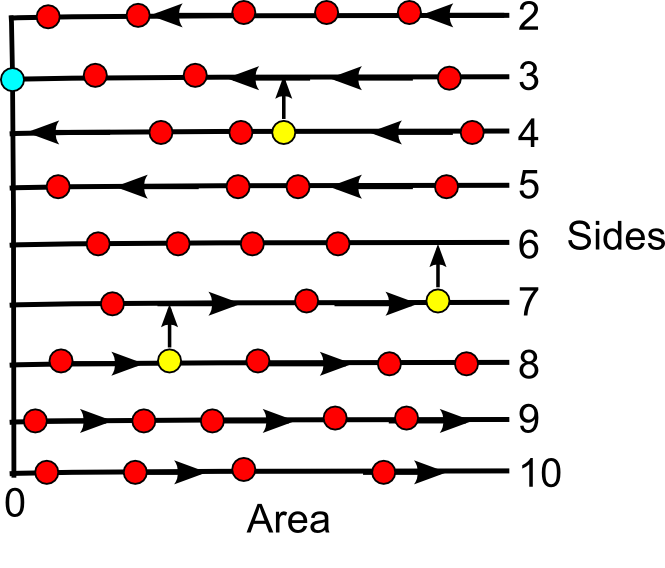
\includegraphics[width = .4\textwidth]{graintops.png} 
 \caption{\textbf{Grain growth via a PDMP}. Particles drift according to their number of sides. Each tier denotes particles of different side numbers. In this instance, a vanishing grain in tier three triggers a  random reassignment  of the number of sides of grains in tiers 4,7, and 8.}
\end{centering}
\end{figure}

\section{Overview}
 
In Chapter 2, we describe a PDMP in generality. We then state its infinitesimal generator $\mathcal A$, and the class of functionals $\mathcal D(\mathcal A)$ that give rise to martingales through the Dynkin formula.    

In Chapter 3, we  study a simplified version of the PDMP described in Section \ref{pdmpgraincoarse}. Here, particles drift on the positive half-line until reaching the origin, where they are reassigned according to a probability density $p(x)$.     We first prove that for empirical densities approaching nonatomic initial conditions, the densities $u(x,t)$ of particles converge to a weak form of the limiting kinetic equation
\begin{alignat}{2}\label{pde1}  
\partial_tu(x,t) - \partial_x u(x,t) = p(x)u(0,t) \quad t, x \in \mathbb{R}^+, \\
u(x,0) = u_0(x) . \nonumber
\end{alignat}
We then focus on constructing measure valued weak solutions of (\ref{pde1}) with mild restrictions on initial data. Finally, we use a popular result of renewal theory to show the existence of an attractor under certain assumptions.

  Chapter 4 is a generalization of PDMPs on grain networks described in Section \ref{pdmpgraincoarse}.  Here, we show the existence of fluid limits of PDMPs that allow generalized rules and probability distributions for particle jumps between different species.  As in Chapter 3, we will show the existence of a weak limit for densities $u_k(x,t)$ on $L_k$, that satisfy the advection-reaction equations
\begin{eqnarray} \label{pde2}
  \lefteqn{\partial_t u_k(x,t)+\partial_{x}(v_k(x)u_{k}(x,t))=  \phantom{u_j(x,t)\mathbf{1}_{R^{(l)}_{ij}}
-K^{(l)}W_k^{(l)}(t)u_k(x,t)}}\label{smoooth}\\
 && \sum_{l = 1}^{M_-}u_l(0,t)v_{l}(0)\left[\sum_{i = 1}^{M}\sum_{j= 1}^{K^{(l)}} W_i^{(l)}(t)u_i(x,t)\mathbf{1}_{R^{(l)}_{ij}=k}
-K^{(l)}W_k^{(l)}(t)u_k(x,t)\right]\nonumber\\ 
&&+\frac{\beta G(t)}{G^{int}(t)}\left( \sum_{i = 1}^{M}\sum_{j= 1}^{K^{int}} w^{int} _iu_{i}(x,t)\mathbf{1}_{R^{int}_{ij} = k}-K^{int}w^{int}_ku_{k}(x,t)
 \right), \nonumber
 \end{eqnarray}
 with initial conditions
 \begin{equation}
u_k(x,0) = u_{k}^0(x), \quad k = 1,\dots, M. \nonumber
\end{equation}
The solutions of (\ref{pde2}) will be shown to be unique in the class of $L^1\cap L^\infty(\mathbb R^+)$ functions.

Finally, in Chapter 5, we return to the problem of grain coarsening. First, we examine the topological behavior of grain networks before and after a grain or side vanishes. After finding a finite set of rules that dictate topological changes,    we then define the various free parameters in the $k$-species model to align with a mean field model for grain coarsening.  Next, we prove some basic properties of the limiting kinetic equation, such as conservation of mass and polyhedral defect.  Finally, we end the chapter with a computational investigation of grain growth, and raise several conjectures about grain statistics.   
  


\clearpage{\pagestyle{empty}\cleardoublepage}

\chapter{An Overview of PDMPs}


\section{PDMPs and generators} \label{pdmpgenerator}
The main class of stochastic processes utilized in this thesis is the piecewise deterministic Markov Process, or PDMP, whose theory is presented in Davis \cite{dav84}.  For a PDMP, a Markov process is allowed deterministic drift along flow lines of a vector field before randomly jumping to a new state.  In addition to covering several examples from queueing theory, including the  M/G/1 queue, the GI/G/1 queue, the model also encapsulates Markov chains.  Our chief object of interest is the infinitesimal generator and martingale from Dynkin's formula associated with the PDMP.   In Chatpers 3 and 4 we plan to use these martingales to provide an approximation to limiting kinetic equations. 


Our goal is to describe a generalized jump process that takes place on a disjoint union of  manifolds, and follows a deterministic drift between jumps. To characterize the state space, we let $\mathcal S$ be a countable set,   $d:\mathcal S\rightarrow \mathbb{N}$ , where for each $\mathbf s \in \mathcal S$,  $M_\mathbf s \subset \mathbb{R}^{d(\mathbf s)}$ is an open set.   The state space is then the disjoint union
\begin{equation}
E =\coprod_{\mathbf s \in \mathcal S} M_\mathbf s = \left\{(\mathbf s, \textbf x):\mathbf s \in \mathcal S,  \textbf x \in M_\mathbf s \subset \mathbb R^{d(\mathbf s)}\right\}. \end{equation}
To define the topology of $E$, let $\iota_\mathbf s:M_\mathbf s \rightarrow E$ be the canonical injection defined by $\iota_\mathbf s(\textbf{x}) = (\mathbf s, \textbf{x})$.  A set $A$ in $E$ is open if for every $\mathbf s$, $\iota_\mathbf s^{-1}(A)$ is open in $M_\mathbf s$. We then define $\mathcal E$ as the Borel sets of $E$. This makes $(E,\mathcal E)$ a Borel space.  

We now define a stochastic process $X(t) = (\mathbf s(t),\zeta(t))$, with a law $(X(t))_{t  \ge 0}$ based on the following:

\begin{enumerate}
\item 
Vector fields $\mathcal X_\mathbf s,\mathbf s \in \mathcal S.$ defined on $M_\textbf s$.
\item
A measurable function $\lambda:E \rightarrow \mathbb R^+$.
\item
A transition measure $Q: \mathcal E \times (E \cup \Gamma^*) \rightarrow [0,1]$.

\end{enumerate}  

We will formally define $\Gamma^*$, the exit boundary of a PDMP, shortly. To see how this fits in with a generalized jump process, points in $M_{\textbf s}$ will travel according to flows defined by $\mathcal X_\mathbf s$ until either a Poisson clock with intensity $\lambda$ rings, or the point hits the boundary of $M_\mathbf s$. When such an event occurs, the point jumps to a new position in $E$, determined by $Q$.   

The vector fields $\mathcal X_\mathbf s$ are chosen so that for every $z \in M_\mathbf s$, there is a unique integral curve $\phi_\mathbf s(t,z)$ satisfying 
\begin{eqnarray}
 \frac d{dt}f(\phi_\mathbf s(t,z)) = \mathcal X _{\mathbf s}f(\phi_\mathbf s(t,z))\\
 \mathbf \phi_\mathbf s(0,z) =  z \nonumber 
\end{eqnarray}
for any smooth function $f: \mathbb{R}^{d(\mathbf s)} \rightarrow \mathbb{R}$.  Here we also require that the vector fields are conservative, meaning that there exists a $t>0$ where $\phi_\mathbf s(r,z)$ is defined for $r \in [0,t]$.   

 Now let $\partial^*M_\mathbf s$ be the exit boundary of $M_\mathbf s$, defined as
  \begin{equation}
 \partial^*M_\mathbf s =\left \{y \in \partial M_\mathbf s: \phi_\mathbf s(t^-, \textbf{x}) = y \quad \hbox{ for some } (t, \textbf{x}) \in \mathbb{R}_+ \times M_\mathbf s\right \}
\end{equation}
 $\Gamma^*$ is then defined as the exit boundary of our state space:
\begin{equation}
\Gamma^* = \coprod_{\mathbf s \in \mathcal S} \partial ^{*}M_\mathbf s 
\end{equation}
At a given state $\mathbf x \in E$, we define the exit time as 
\begin{equation}
t^*(\mathbf x) = \inf \{t >0: \phi_\mathbf s(t, \textbf{x}) \in \partial ^{*}M_\mathbf s\}.  
\end{equation}
The stochastic process $(X(t))_{t \ge 0}$ with initial condition $X(0) =  (\mathbf s,z)$ is then defined as follows.  For $\mathbf x = (\mathbf s, z)$, define a survivor function $\mathcal F$ as 
\begin{equation}
\mathcal F_{\mathbf x}(t) = \begin{cases} \exp\left(-\int_0^t \lambda(\mathbf s,\phi_\mathbf s(r,z))dr\right), & t<t^*(\textbf{x}), \\ 0, & t \ge t^*(\textbf{x}).
\end{cases} 
\end{equation}
The rate \ $\lambda:E \rightarrow \mathbb R^+$ is a measurable function, where for every state $\textbf{x} = (\mathbf s,  \textbf{x}) \in E$ there exists $\varepsilon > 0$ where the function $s \rightarrow \lambda(\mathbf s, \phi_\mathbf s(s, \textbf{x}))$ is integrable for $s \in [0,\varepsilon)$.  We also define $Q(A;\textbf{x})$ to be a measurable function of $\textbf{x}$ for each fixed $A \in \mathcal E$ on $\textbf{x} \in E \cup \Gamma^*$, and a probability measure on $(E, \mathcal E)$ for each $X \in E \cup \Gamma^*$.


Now choose a random variable $T_1$ such that $\mathbb{P}[T_1>t] = \mathcal F_\mathbf x(t)$.  Now independently choose an $E$-valued random variable $(L,Z)$ with distribution $Q(\cdot ; \phi_\mathbf s(T_1,z))$.  The trajectory of $X(t)$ for $t \le T_1$ is then
\begin{equation}
X(t) = \begin{cases} (\mathbf s,\phi_\mathbf s(t,z)), & t<T_1 \\
(L,Z), & t = T_1.
\end{cases}
\end{equation}
From $X(T_1)$, we choose the next inter-jump time $T_2-T_1$ and $X(T_2)$ in a similar fashion. It can be shown that the process $X(t)$ is Markov, and in fact, strong Markov (Section 3 of \cite{dav84}).  

As a Markov process, the PDMP has an associated infinitesimal generator $\mathcal A$, acting on a domain $\mathcal D(\mathcal A)$, defined as the set of functions $f:E\rightarrow \mathbb R$ where the limit 
\begin{equation}
 (\mathcal Af)(\mathbf x)=  \lim_{t\rightarrow 0^+} \frac{\mathbb E^\mathbf x (f(X(t)))-f(\mathbf x)}{t}
\end{equation}
exists for all $\mathbf x \in E$. The infinitesimal generator then takes the form

\begin{equation}\label{generator}
\mathcal Af(\mathbf x) = \mathcal X(f(\mathbf x))   +\lambda(\mathbf x)\int_E (f(y)-f(\mathbf x))Q(dy;\mathbf x)), \quad f \in \mathcal D(\mathcal A).
\end{equation}
From here, we can use Dynkin's formula to derive the  
martingale
\begin{equation}\label{martingale}
M_t^f := f(X(t)) - f(X(0))-\int_0^t \mathcal A f(X(s))ds,\quad f \in \mathcal D(\mathcal A).
\end{equation}

The following set of sufficient conditions for membership in $\mathcal D(\mathcal A)$ is given in Rolski et. al. \cite{rolski2009stochastic}
\begin{theorem}\label{fourcond} A function $f: E \rightarrow \mathbb{R}$ satisfies $f \in \mathcal D(\mathcal A)$ if the following hold:
  
\begin{enumerate}
\item 
The function $t \rightarrow f(\phi(x,t))$ is absolutely continuous on $[0,s^*(x))$ for every $\mathbf x \in E$, where $s^*(x) = \inf_t\{t|\mathcal F(t) =0\}$. \item
$f(x)  = \lim_{t \rightarrow 0} f(\phi(x,t))$ exists for all $x \in  \Gamma^*$ \item
(Boundary condition):$f(x)= \int_E f(y) Q(dy,x)$ for $x \in \Gamma^*$\item
(Finite expectation of number of jumps): for all $t \in \mathbb{R}^+, x\in E$,
\begin{equation} 
\mathbb{E}\left[\sum_{i = 1}^{m(t)} |f(X(T_i)-f(X(T_{i-1}))|\right]<\infty
\end{equation}
\end{enumerate}
\end{theorem}

\subsection{A note on Skorokhod topologies} \label{j1m1}

\begin{figure}
\begin{centering}
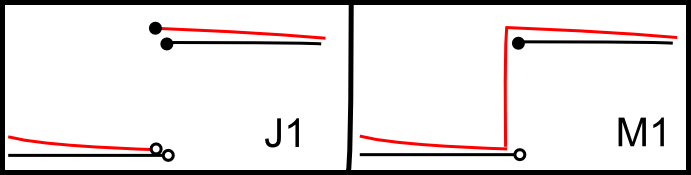
\includegraphics[width=.5\textwidth]{j1m1tops.png}
\caption{\textbf{Topologies for cadlag functions.} \textbf{Left:} Two functions that are ``close" in the J1 topology.  Note that the magnitude of their jumps are similar. \textbf{Right:} Two functions close in the M1 topology.  Jumps are not required to be close in this case, but rather the Hausdorff distances of each function's completed graph. }\label{j1m1}
\end{centering}
\end{figure}

Throughout this thesis, our focus will be on stochastic processes which are cadlag, or are right continuous with lefthand limits. Let $(\mathfrak M,d)$ denote a metric space with metric $d$.   In the following, we use the $J1$ Skorohod topology, denoted $\mathbb D([0,t],\mathfrak M)$. For our purposes, $\mathfrak M$ will either be $\mathbb{R}^+$ or  $\mathcal M(\mathbb{R}^+)$, the space of finite measures on $\mathbb{R}^+$ with the Prohorov metric \cite{billingsley2009convergence}.
The $J1$ topology  allows for convergence of functions that ``wiggle" in time as well as space, and has  the following characterization (see \cite{jac87}): 

Let $\mathscr R$ be the set of continuous reparameterizations $r: [0,t]\rightarrow \mathbb{R}^+$: functions that are strictly increasing, where $r(0) = 0$ and $r(t)=t$.  A sequence of functions $\alpha_n \rightarrow \alpha$ in $\mathbb{D}([0,t],\mathfrak M)$ if and only if there is a sequence $r_n \in \mathscr R$ with 

\begin{enumerate}
\item $\sup_s |r_n(s)-s| \rightarrow 0,$
\item $\sup_{s \le t} d(\alpha_n(r_n(s)), \alpha(s)) \rightarrow 0.$ 
\end{enumerate}
as $n \rightarrow \infty$. If $\alpha(t)$ is continuous, the functions actually converge in the local uniform topology. However, in general,  the local uniform topology is strictly stronger than the Skorohod J1 topology, but this fact won't be used, since limiting functions of our interest in this paper will have no jumps (see Remark \ref{unifremark}).  



\clearpage{\pagestyle{empty}\cleardoublepage}

\chapter{Kinetic Limits of Piecewise-Deterministic Markov Processes: The Dynamic Shuffler}
%&latex












\section{Introduction}



This chapter examines an instance of a PDMP, called the \textbf{$N$ particle dynamic shuffler,}  which tracks $N$ particles on the positive real line moving with velocity -1 until reaching the origin.  Upon hitting the origin, a particle is randomly redistributed back to $\mathbb{R}^+$, with respect to a probability density $p(x)$ in $\mathbb R^+$. If initial empirical densities of $N$ particles approach a limiting density $u_0(x)$, we will show that the random densities of the $N$ particle dynamic shuffler at time $\tau>0$ approach a deterministic density $u(x,\tau)$, which satisfies a weak form of a one-dimensional transport equation with source term, 
\begin{alignat}{2}  \label{pde}
\partial_\tau u(x,\tau) - \partial_x u(x,\tau) = p(x)u(0,\tau) \quad \tau, x \in \mathbb{R}^+, \\
u(x,0) = u_0(x) . \nonumber
\end{alignat}
 In this chapter, we will refer to (\ref{pde}) as the \textbf{redistribution equation}.  Regularity conditions on $u_0(x)$ and $p(x)$ largely depend on the types of solutions we seek, and will be considered throughout this chapter.

  
  


We will borrow methods from coagulation theory. For instance, consider the one-dimensional Allen-Cahn equation $\partial_t u = \partial_{xx} u+u-u^3$, which describes a coagulation process on the real line. Specifically, given an interval partition of $\mathbb R$, the smallest interval merges with its two neighbors to form a single interval, and the process continues. Menon, Niethammer, and Pego used the Allen-Cahn equation as a source of motivation in \cite{menon2010dynamics},  investigating a wide range of clustering events.  The discrete nature of these clustering phenomena  suggested that it was reasonable to seek measure-valued solutions.  Such solutions, continuous in time in the space of probability measures, were found using an intrinsic time scale based on the number of clusters in the system.  The same philosophy will be applied to (1), which will use the time scale
of the total number of visits to the origin by particles,
\begin{equation}\label{cov}
t = \int_0^{\tau} u(0,s)ds.
\end{equation}
   We should note that while the tools used in coagulation theory prove useful to this chapter, in general there is no coagulation occurring in the redistribution equation!  The total number of particles $N(\tau)= \int_{\mathbb{R}^+}u(x,\tau)dx$ is preserved, while the total mass, or first moment, $M(\tau) = \int_{\mathbb{R}^+} xu(x,\tau)dx$ can potentially change in time.

The sections of this chapter are arranged as follows.  In Section \ref{stochlimit}, we derive (\ref{pde}) as a limit of densities of the $N$ particle dynamic shuffler. This is done by exploiting the infinitesimal generator, and building a martingale approximation to (\ref{pde}). Section \ref{lapsection} derives a solution formula for (\ref{pde}) for smooth initial conditions through the Laplace transform.
We then use the change of variables (\ref{cov}) in Section \ref{meassect} to derive a measure-valued solution formula for (\ref{pde}).  A specific example is presented in  Section \ref{ptmass}, with initial data a point mass. Sections \ref{strongsection} and \ref{weaksection} prove well-posedness of weak and strong solutions for (1), meaning that the solution formulas of Sections \ref{lapsection} and \ref{meassect} are well-defined. In  Section \ref{statio}, we conclude the chapter by   providing asymptotics for $u(x,\tau)$ via the key renewal theorem from renewal theory. 


  
    
\begin{figure}
\begin{centering}
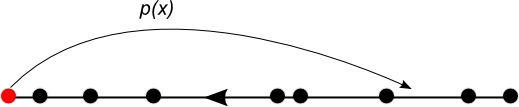
\includegraphics[width=.5\textwidth]{1dredistribution.png}
\caption{\textbf{A dynamic shuffler.} Particles (black dots) drift left with unit speed until hitting the origin, where a particle (red dot) is redistributed according to a density $p(x)$.}
\end{centering}
\end{figure}


    

 
\section{A solution via a stochastic limit}\label{stochlimit}
A discrete approximation of the behavior underlying  (\ref{pde}) can be obtained through PDMPs.  In the following section, we show the dynamic shuffler of $N$ particles is a PDMP, and then take a fluid limit as $N \rightarrow \infty$. In this limit, particle densities will converge to a weak version of (\ref{pde}).    

 

Our process is as follows.  Let particles $x_1, \dots, x_N \in \mathbb{R}^+$ be given. Each particle moves left with unit speed until a particle hits the origin.  This particle is randomly assigned a new location according to a probability distribution function $p(x) \in C^1(\mathbb{R}^+)$. The shuffler continues as before, with particles drifting until a new particle hits the origin. 

We will now show that this process can be interpreted as a PDMP.  The general theory and notation of a PDMP is discussed in  Section \ref{pdmpgenerator}.  From the viewpoint of a dynamic shuffler with $N$ particles, our state space is $E^N = \mathbb{(R^+)}^N$, with a state written as
\begin{equation}
\mathbf x = (x_1, \dots, x_N) \in E^N.
\end{equation}
 There is no need to consider disjoint copies of $E^N$. This is because particles are neither created nor destroyed, and there is only one vector field, corresponding to each particle having velocity of $-1$, namely $\mathcal X= -\sum_{i = 1}^N\frac{\partial}{\partial x_i}$.  Since all jumps  occur on the boundary of $E$, where there is a particle at the origin, we have zero jump frequency: $\lambda \equiv 0$. For an element $y \in \partial \Gamma^*$ of the form
\begin{equation}
y= \{y_1, \dots, y_{i-1},0, y_{i+1} \dots, y_N\},
\end{equation} 
the transition kernels satisfy
\begin{equation}
Q(\mathbf x,y) = \begin{cases}p(z), & \mathbf x= (y_1,\dots, y_{i-1},z,y_i,\dots, y_N), \\
0, & \hbox{otherwise.} \\
\end{cases}
\end{equation}
 We thus have a well defined PMDP  $x(t) = (x_1(t), \dots, x_N(t))$ on $E^N$. 
At each time $t >0$, we define the random empirical measure process of particle locations: 
\begin{equation}
\nu^N_t (dx) = \sum_{i = 1}^N \frac{\delta_{x_i(t)}}{N}(dx).  \nonumber
\end{equation}
Let $\phi \in C^1(\mathbb{R}^+)$, we can pair an arbitrary finite measure $\mu \in \mathcal P(\mathbb R^+) $ through integration:  
\begin{equation}
\langle \mu, \phi \rangle = \int_{\mathbb{R}^+}\phi(x) \mu(dx). \nonumber
\end{equation} A natural choice for  a functional of our PDMP is the empirical pairing $F^N(\phi):E \rightarrow \mathbb{R}^+$, defined by 
\begin{equation}
F^N(\phi)(\mathbf x) = \sum_{i = 1}^N \frac{\phi(x_i)}{N} .  \end{equation}

As a Markov process, the PDMP has an associated generator and martingale determined from Dynkin's formula. Our aim is to define a non-trivial set of test functions such that $F^N(\phi)(\mathbf x)\in \mathcal D(\mathcal A)$,    the domain of valid functionals for the infinitesimal generator $\mathcal A$.  We will use the sufficient conditions given in Theorem \ref{fourcond}.  

 
The major hurdle to show $F^N(\phi) \in \mathcal D(\mathcal A)$ is in  boundary condition (3) of Theorem 2, which is equivalent to proving 
\begin{equation}
\mathbb{E}\left[\Delta F^N(\phi)(y)\right] = 0, \quad y \in \Gamma^*,
\end{equation}
where, if a random variable $Z(y)$ is distributed in $E$ with respect to $Q(\cdot,y)$, then  
\begin{equation}
\Delta F(y) = F(Z(y))-F(y).
\end{equation}
In order for  condition (3) to hold, we must equate the value of a particle at the origin,  $\phi(0),$ with its expected value when it is redistributed back to $\mathbb R^+$. We thus use the space of test functions  
\begin{equation}
\mathcal  C  \ = \left\{\phi \in C^1(\mathbb{R}^+) \mid \phi(0) = \int_0^\infty \phi(x)p(x)dx, \quad \|\phi'\|_\infty<\infty \right\} . \end{equation}
It's straightforward to show, using the regularity of $\phi \in \mathcal C$, that our empirical functional $F^N(\phi)$,  is  in the domain $\mathcal D(\mathcal A)$. Vector fields satisfy, by the chain rule,
\begin{equation}
\mathcal X(F^{N}(\phi)(\mathbf x)) = \sum_{i = 1}^{N}-\frac{\partial}{\partial x_i}\frac{\phi(x_i)}{N} = -\sum_{p_i \in T_k} \frac{\phi'(x_i)}{N} 
 = -\langle \nu_s^N, \phi'  \rangle. 
\end{equation}
   The martingale $M_\phi^N(t)$ associated with $F^N(\phi)$ given in (\ref{generator}) and (\ref{martingale}),   then satisfies 
\begin{equation}\label{marty}
M^N_\phi(t) = \langle \nu_t^N,\phi \rangle- \langle \nu_0^N,\phi \rangle- \int_0^t \langle \nu_s^N,\phi' \rangle ds . 
\end{equation}



   


It is of note that if we allow for initial empirical data to converge to measures with jumps in its cumulative distribution function, then we should not expect convergence in the $J1$ topology. Indeed, if we initial empirical densities densities that approach a point mass,  redistribution of particles concentrate during increasingly small time intervals. During this interval, the value $F^{N}(\phi)(X(t))$ forms an approximately continuous ``monotone staircase" between $\phi(0)$ and $\mathbb{E}[\phi(X)]$ whose jumps do not approach that of the limiting function (see Fig. \ref{topcounter})

The right topology to invoke in this case is the Skorokhod M1 topology, a weaker version of the J1 topology. Convergence of functions in this case is characterized by measuring the distance between the completed graphs of cadlag functions.  In particular, continuous functions can approximate a function with jumps.  We refer the reader to \cite{whitt2002stochastic} for a rigorous explanation of the $M1$ topology, as well as its relation to the $J1$ topology.   We withhold a discussion of $M1$ convergence of the redistribution equation for now, and hope to address the issue in future work.  Thus, in this exposition, our initial empirical measures will approach nonatomic measures.  
\begin{figure}
\begin{centering}
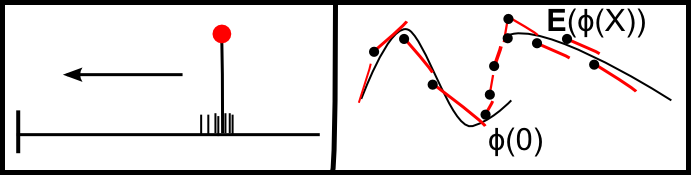
\includegraphics[width=.5\textwidth]{topcounter.png} 
\caption{\textbf{M1 convergence of measure valued initial data.}  \textbf{Left: }Particles (small vertical segments) approximating a point mass (segment with red dot) drift toward the origin. \textbf{Right:} The value of $F(\phi)(x)$ before and after particles hit the origin. As the number of particles grows, their jumps form a ``monotone staircase" connecting the jump of the limiting functional.}\label{topcounter}
\end{centering}
\end{figure}





\subsection{Convergence of empirical processes}

 We are now ready to state our main theorem.  It may be seen as a  law of large numbers limit for random empirical densities. 

\begin{theorem}\label{pdmpproof}
Suppose we have weak convergence of initial empirical measures $\nu_0^n \rightarrow \nu_0 $, where $\nu_0 $ is nonatomic.  Then the random measure process $\nu_t^N$ converges to a deterministic limit $\nu_t$ under the Skorokhod topology $\mathbb D([0,t], \mathcal P(\mathbb{R}^+))$. The limiting measure satisfies the kinetic equation
\begin{equation}\label{limeq1}
0= \langle \nu_t,\phi \rangle- \langle \nu_0,\phi \rangle- \int_0^t \langle \nu_s,\phi' \rangle ds \quad 
\end{equation}
for every $\phi \in \mathcal C$.

\end{theorem}
The following two lemmas will help in establishing tightness \cite{roelly1986criterion,joffe1986weak}.


\begin{lem}\label{Cap}
Let $T>0$. A sequence $\nu_k(t)$ in $\mathbb D([0,T], \mathcal M(\mathbb{R}^+))$ is tight if and only if the sequence of functions $\langle \phi, \nu_k(t) \rangle$ is tight in $\mathbb D([0,T],\mathbb{R}^+)$ for all $\phi \in C_b(\mathbb R^+)$.
\end{lem}



\begin{theorem}\label{Ald}
 (\textbf{Aldous' conditions}) Let $T>0$. A sequence of stochastic processes $X_n(t)$ is tight in  $\mathbb D([0,T],\mathbb{R}^+)$ if the following two conditions hold:
\begin{enumerate}
\item For all rational $t \in [0,T)$ and for all $\varepsilon > 0$, there exists an $L>0$ such that
\begin{equation}
\sup_{n>0} \mathbb{P}(|X_n(t)|>L) \le \varepsilon.
\end{equation}
\item For jump times $\tau_1, \dots, \tau_{m(t)}$, then for all $\varepsilon >0$,
\begin{equation}
\lim_{r \rightarrow 0} \limsup_{n \rightarrow \infty} \sup_{s<r,\tau_{i}}  \mathbb P(|X_n((\tau_i+s) \wedge T) - X_n(\tau_i)| > \varepsilon) = 0.
\end{equation}
\end{enumerate}
\end{theorem} 

Combining the two statements, we need to show that, for a fixed $\phi \in C_b(\mathbb R^+),$ the sequence of random variables $X_n(t) = \langle \phi, \nu_t^N \rangle $ satisfies Aldous' conditions. 



Before showing the next lemma, we define the set of intervals of width less than $\delta>0$:
\begin{equation}
I_\delta = \{(a,b)\subset \mathbb{R}^+, b-a<\delta\}.
\end{equation}
\begin{lem}\label{tech} Let $T>0$.  Suppose $\nu_0^N \rightarrow \nu_0$ weakly, and $\nu_0$ is nonatomic. Then for all $\eta > 0$, 
\begin{equation}\label{paccon}
 \lim_{\delta \rightarrow 0} \sup_{I \in I_\delta}\limsup_n \sup_{t \in [0,T]}\mathbb P(\nu_t^N(I) >\eta)) = 0 .
\end{equation}
\end{lem}

\begin{proof}
Let $\eta > 0$. For $T = 0$, we have that (\ref{paccon}) follows from the fact that $\nu_0$ is nonatomic.
% \begin{equation}\label{zerocase}
% \lim_{\delta \rightarrow 0}\limsup_n\nu_0^n(I_\delta) = 0
% \end{equation}
% 
% for all $\delta$ intervals $I_\delta$.
% 
% Suppose, for contradiction, that this were not the case.  This means for each $M \in \mathbb{N}$, there is a subsequence $\nu_0^{n_k^M}$ and intervals $I_{1/M}$ that satisfy $\limsup_{n_k^M}\nu_0^{n_k^M}(I_{1/M}) \ge \eta$, which implies $\lim_{n\rightarrow \infty} \nu_0^n(I_{1/M}) \ge \eta$.  Let $L>0$ so that $\nu_0([L,\infty))= \eta/2.$  Note that only finitely many sets $I_{1/M}$ lie in $[L,\infty)$.  Otherwise, 
%  
%  $$1-\eta/2 = \nu_0([0,L)) = \lim_{n\rightarrow \infty} \nu_0^n([0,L))\le1-\eta,$$
%  a contradiction.  Now let $p_M$ denote the centers of the intervals $I_{1/M}$.  Since $[0,L]$ is compact, we have a cluster point $p$ of the sequence $p_k$ . Therefore, any interval containing $p$ contains infinitely many intervals $I_{1/M}$. We then have
%  
%  $$0 = \nu_0(p) = \lim_{n \rightarrow \infty} \nu_0([p-1/n,p+1/n]) = \lim_{n \rightarrow \infty} \lim_{k \rightarrow \infty} C^k_0([p-1/n,p+1/n])>\eta,$$
% which is our desired contradiction.  Thus (\ref{zerocase}) holds.

We now show (\ref{paccon}) for $s \in \mathbb{R}^+$. For $S\subset \mathbb{R}$  , we denote $S+s = \{x \in \mathbb{R}|x-s \in S\}$. Now let $T>0$.  For $t\in [0,T]$, $\nu_t^N(I)$ is equal to the sum of $\nu_0^n(I+t)$ and the sum of masses that are redistributed to $I+t-s$ at time $s$.

To estimate redistribution probabilities, we focus on the location of a single particle $x(t)$ for $t \in [0,T].$ Let 
\begin{equation}
M_\delta = \sup_{x \in \mathbb R^+} \int_x^{x+\delta}p(s)ds.
\end{equation}
Note that because $p \in L^1(\mathbb{R}^+)$, $M_\delta \rightarrow 0$ as $\delta \rightarrow 0$. Now,  the probability of $x(t) \in I$ is bounded by the number of jumps that $x(t)$ undergoes, multiplied by the probability that the next jump lands in the correct $\delta$ interval, or
\begin{eqnarray}
\mathbb{P}(x(t) \in I) \le \sum_{k = 0}^\infty\mathbb{P}(x(t) \hbox{ has $k$ jumps})M_\delta\\
\le M_\delta\sum_{k = 0}^\infty \mathbb{P} \left(\sum_{i = 1}^k X_i <t)\right),\nonumber
\end{eqnarray}
where $X_i, i \in \mathbb N$ is a sequence of i.i.d random variables distributed with respect to $p(x)$.
A Chernoff-type bound shows that the sum over $k$ converges.  Indeed, we have
\begin{eqnarray}\label{chernoff}\mathbb{P} \left(\sum_{i = 1}^k X_i <t\right) =\mathbb{P} \left(\exp\left(-\sum_{i = 1}^k X_i) \right)>\exp(-t)\right)\\
\le e^{t}\mathbb{E}[e^{-X_1}]^k, \quad k \in \mathbb N,\label{expseries} \nonumber
\end{eqnarray}
by Markov's inequality. The series of  terms (\ref{expseries})  is then  summable over $k$ to a finite constant, denoted $K$.
As particles $x_1(t), \dots,x_n(t)$ behave independently, we now have an estimate for  $\nu_t^N(I)$, given by 
\begin{equation}
 \mathbb{E}[\nu_t^N(I)] \le Ke^tM_\delta. \nonumber
\end{equation}
But then we have, from Markov's inequality,
\begin{eqnarray}
\lefteqn{\sup_{t \in [0,T]}\mathbb{P}( \nu_t^N(I)>\eta)}\\ &&\le  \sup_{t \in [0,T]}\mathbb{P}( \nu_t^N(I)>\eta)  
 \le\sup_{t \in [0,T]}\frac{\mathbb{E}[ \nu_t^N(I)]}{\eta}\nonumber\\&&\le \frac{Ke^TM_\delta}{\eta}  \ \rightarrow 0\quad  \hbox{ as  } \delta \rightarrow 0 \nonumber
\end{eqnarray}
\end{proof}

From here the proof for Aldous' conditions is straightforward.
\begin{theorem} For $\phi \in \mathcal C$, the Aldous conditions in  Theorem \ref{Ald} hold for $\langle\nu, \phi\rangle$
\end{theorem}
\begin{proof}

Condition 1: This follows trivially since $\langle\phi, \nu_t^N\rangle \le \|\phi \|_\infty$, meaning that $L = \|\phi\|_\infty$ satisfies Condition 1.

Condition 2:   We have
\begin{eqnarray}
|\langle\phi,\nu_{\tau+s \wedge T}^N\rangle \  - \langle\phi,\nu_{\tau}^N\rangle| = \left| \int_{\mathbb{R}^+}\phi(x) (\nu_{\tau+s\wedge T}^N - \nu_\tau^N)(dx)\right | \\
\le \left | \int_s^\infty (\phi(x-s)-\phi(x))\nu_\tau^N(dx)  \right|+\|\phi\|_\infty \nu_{\tau}^N([0,s]). \nonumber
\end{eqnarray}
Since $\phi$ is continuous, the first term approaches 0 as $s \rightarrow 0$, and by Lemma \ref{tech}, we have that for any $\varepsilon >0$, 
  \begin{equation}
 \lim_{s \rightarrow 0}\limsup_N\sup_{\tau \in [0,T]}\mathbb P( \nu _{\tau}^N([0,s])>\varepsilon/\|\phi\|_\infty) = 0,     
\end{equation} 

which verifies Condition (2), and completes our proof.
\end{proof}

We will now take care of the martingale term, which we can show is bounded in the local uniform metric:


\begin{theorem}\label{martyproof}
The martingale term $M^\phi_N $ in (\ref{marty}) is bounded by 
\begin{equation}
\mathbb{E}\left[\sup_{s \in [0,t]}(M_N^\phi(s))\right] \le \frac{Be^{t/2}\|\phi\|_\infty}{\sqrt N},
\end{equation}
where $B$ is a constant determined by a summable series.
\end{theorem}

\begin{proof} 
We first note that
\begin{equation}
|\Delta M_N^\phi(t) |= |M_N^\phi(t)-M_N^\phi(t^-)| = |\Delta\langle \nu_t^N,\phi\rangle| \le \frac{2\|\phi\|_\infty}N 
\end{equation}
It then follows, for $d_N(t)$ denoting jump times $\tau_1, \dots, \tau_{d_N(t)}$, that
\begin{eqnarray}
\mathbb E\left[M_N^\phi(t)^2\right] = \mathbb{E}\left[\sum_{i = 1}^{d_N(t)}\Delta M_N^\phi(\tau_i)^2\right]\\
\le\frac{4\|\phi\|_\infty^2}{N^2} \mathbb{E}[d_N(t)]\nonumber
\end{eqnarray}
Here we again appeal to Chernoff bounds in (\ref{chernoff}) to help estimate the total number of jumps that occur. Let $x(t)$ denote the stochastic process tracking a tagged  particle.  This gives us 
 \begin{eqnarray}
 \mathbb{E}[\#\{\hbox{jumps for } p(t)\}] = \sum_{k = 0}^\infty k \mathbb{P}(p(t) \hbox{ jumps $k$ times})\\
\le k\mathbb{P}\left(\sum_{i = 0}^k X_i \le t\right)\le e^t \sum_{k = 0}^\infty k\mathbb{E}[e^{-X_1}]^k\le Ce^t \nonumber 
\end{eqnarray} 
for some constant $C$.  This gives us $\mathbb E[d_N(t)] \le CNe^t$, meaning
\begin{equation}
\mathbb{E}[M_N^\phi(t)^2] \le  \frac{4Ce^t\|\phi\|_\infty^2}{N}.
\end{equation}

Now, using Doob's inequality, we obtain
\begin{equation}
\mathbb{E}\left[\sup_{s \le t}|M_N^\phi(s)|\right]^2 \le \mathbb E\left[\sup_{s \le t} M_N^\phi(s)^2\right] \le 4\mathbb E[M_N^\phi(t)^2]
\end{equation}
Setting $B =4 \sqrt C$ then gives our desired result.
\end{proof}

Since we have shown tightness, we can extract a subsequence $\nu_t^{N_k} \rightarrow \nu_t$ in the Skorokhod J1 topology.  Furthermore, since local uniform  convergence is stronger than convergence under the Skorokhod topology, we also have $M_{N_k}^\phi(t) \rightarrow 0$ in $\mathbb D([0,T], \mathbb{R})$.  Thus our limiting measure $\nu_t$ satisfies equation (\ref{limeq1}).

We now finish the proof of Theorem \ref{pdmpproof} by showing uniqueness of limits.  This will be done by approximating the measure processes PDMP $X^N(t)$ by processes $X^{N,\varepsilon}(t) = (x_1^{N,\varepsilon}(t), \dots, x_N^{N,\varepsilon}(t))$ with perturbed redistribution probabilities $p_\varepsilon(t)$, given by
\begin{equation}
p_\varepsilon(x) = \begin{cases}0 & x \in [0,\varepsilon]  \\
\frac{p(x)}{\int_\varepsilon^\infty p(y)dy} & x >\varepsilon.\\
\end{cases}
\end{equation}
These redistributions are probabilities of a particle redistributed with respect to $p$, conditioned on being redistributed in $[\varepsilon, \infty)$.  Suppose now that for time $t \in [0,\varepsilon]$, we have random processes $\nu_t^{N,\varepsilon}$ given by  
\begin{equation}
\nu_t^{N,\varepsilon} = \sum_{i = 1}^N \frac{\delta_{x_i^{N,\varepsilon}(t)}}{N}. \end{equation}
If for some nonatomic $\nu^{\varepsilon}$ we have convergence of initial measures $\nu^{N,\varepsilon} \rightarrow \nu^\varepsilon$ in the $J1$ topology, then there is a unique deterministic measure valued limit $\nu_t^\varepsilon$ of $\nu_t^{N, \varepsilon}$.  For any open interval $A$, 
\begin{equation}
\nu_t^\varepsilon(A) = \nu_0^\varepsilon(A+t) +\int_0^t\int_Ap_\varepsilon(x+t-s)dxdF_{\nu_0^\varepsilon}(s),
\end{equation}
where $F_{\nu_0^\varepsilon}(s)$ is the cumulative distribution function of $\nu_0^\varepsilon$ for time $s \in [0,\varepsilon)$.  That we have such a deterministic formula comes from the fact that when $t \in [0,\varepsilon]$, particles only redistribute once. Thus, the total amount of  redistributed mass at time $t$ is exactly equal to $F_{\nu^\varepsilon(t)}$. The uniqueness actually extends for all time $t \in [0,\infty)$, since we can extend our unique solution to time $2\varepsilon$ by setting initial conditions equal to $\nu^\varepsilon_\varepsilon$, and so forth. 

Let $L^N_\varepsilon(t)$ and $|L^N_\varepsilon(t)|$ denote the support and number, respectively,  of particles which at some time hit the origin and are redistributed to $[0,\varepsilon]$ in time $[0,t]$. We now split the process $\nu^N_t$ by which   particles are in $L^N_\varepsilon(t):$
   \begin{equation}\label{meassplit}
  \nu_t^N =\frac{N-|L_\varepsilon^N(t)|}{N} \sum_{a_i^{N}(t) \notin L_\varepsilon^N(t)}\frac{\delta_{a_i^N(t)}}{N-|L_\varepsilon^N(t)|}+ \sum_{a_i^{N}(t) \in L_\varepsilon^N(t)}\frac{\delta_{a_i(t)}}{N}.\\ \end{equation}
Now we use the martingale bounds from Theorem \ref{martyproof} to see that
\begin{eqnarray}
  \mathbb{E}[\frac{|L_\varepsilon^N(t)|}{N}]\le \frac{\mathbb{E}[d_N(t)]}{N}
\int_0^\varepsilon p(x)\\\le  Be^t \int_0^\varepsilon p(x) \rightarrow 0 \quad   \quad \hbox{ as }\varepsilon\rightarrow 0\nonumber
\end{eqnarray}
 Therefore, the second term in (\ref{meassplit}) approaches 0 in $L^1$. Notice, however, that particles not in $L_\varepsilon^N(t)$ are distributed with respect to  $p_\varepsilon$. Thus, we have , for identical initial empirical measures $\nu_0^N =\nu_0^{N, \varepsilon}$, then for any open interval $A \subset \mathbb{R}^+$, we have
\begin{equation}
\mathbb{E}\left[\sup_{s \in [0,t]}| \nu^N_s(A)- \nu_s^{N,\varepsilon}(A)|\right] \rightarrow 0 \quad \hbox{ as } \varepsilon \rightarrow 0
\end{equation}

For subsequences $n_1(N)$ and $n_2(N)$ with $n_i(N)\rightarrow \infty$ as $N\rightarrow \infty$ for $i = 1,2$, suppose that we had two converging subsequences $\nu^{n_1(N)}_t\rightarrow  \nu_t$ and $\nu_t^{n_2(N)}\rightarrow \tilde \nu_t$ in $\mathcal P(\mathbb{R}^+)$. Applying the triangle inequality then yields, 
 \begin{eqnarray}
 \lefteqn{\mathbb{E}\left[\sup_{s \in [0,t]}|\nu_s(A)-\tilde \nu_s(A)|\right]}\\
 &&\le \mathbb{E}\left[\sup_{s \in [0,t]}|\nu_s(A)- \nu_s^{n_1(N)}(A)|\right]+\mathbb{E}\left[\sup_{s \in [0,t]}|\tilde \nu_s(A)- \nu_s^{n_2(N)}(A)|\right]\nonumber\\
&&+\mathbb{E}\left[\sup_{s \in [0,t]}|\nu_s^{n_1(N)}(A)-\nu_s^{n_1(N),\varepsilon}(A) |\right]+\mathbb{E}\left[\sup_{s \in [0,t]}|\nu_s^{n_2(N)}(A)-\nu_s^{n_2(N),\varepsilon}(A) |\right] \nonumber\\
&&+\mathbb{E}\left[\sup_{s \in [0,t]}| \nu_s^{n_1(N),\varepsilon}(A)-\nu_s^{n_2(N),\varepsilon}(A) |\right]. \nonumber
\end{eqnarray} 
   As $n$ and $\varepsilon$ were arbitrary, if we take limits of $N \rightarrow \infty$, and then $\varepsilon \rightarrow 0$ , we see that in fact $\nu_s = \tilde \nu_s$. 








\section{A solution via the Laplace transform}\label{lapsection}

The goal for the rest of this chapter is to generalize (\ref{pde}) for a larger class of initial conditions, and prove a basic result about a universal attractor.  Our hope is that such an analysis will highlight the use of several techniques that may be utilized for more complicated PDMPs. The existence of universal attractors is a sought after problem in coarsening systems, such as Smoluchowski's coagulation equation \cite{menon2004approach} and grain boundary coarsening \cite{her12}. 

We begin our study of (\ref{pde}) by noting that the rate of redistribution in (\ref{pde}) is given by the local quantity $u(0,\tau)$.  This, if not already evident, becomes clear when we integrate along characteristics $x(\tau) = x_0-\tau$, giving us the integral form of the redistribution equation:
\begin{equation}\label{intsol}
u(x,\tau) = u_0(x+\tau) +\int_0^\tau p(x+\tau-s)u(0,s)ds. 
\end{equation}
Thus, well-posedness of (\ref{intsol}) ultimately depends on the behavior of $u(0,s)$.
Throughout this chapter, we'll use the Laplace transform  
\begin{equation} v(q,\tau) := \int_{\mathbb{R^+}}e^{-qx}u(x,\tau)dx. 
\end{equation}
We use the identity for the Laplace transform of $u_x$,  
\begin{eqnarray}\label{lapux}
\int_{\mathbb{R^+}}e^{-qx}u_x(x,\tau)dx = \int_{\mathbb{R^+}}\partial_x(e^{-qx}u(x,\tau))-\partial_x(e^{-qx})u(x,\tau)dx\\
 = q\int_{\mathbb{R^+}}e^{-qx}u(x,\tau)dx - u(0,\tau) = qv-u(0,\tau) \nonumber 
 \end{eqnarray}
 Denoting $\mathcal L(f)$ as the Laplace transform of  $f$ ,  (\ref{lapux}) then gives us
\begin{align*}
\mathcal{L}(u_\tau-u_x) = \dot v-qv+u(0,\tau), \hbox{ and }   \\
\mathcal L(p(x)u(0,\tau)) = \bar P(q)u(0,\tau),
\end{align*}
where we define $ \bar P(q)$ to be the Laplace transform of $p(x)$.  We now have (\ref{pde}) in the Laplace variable $v$,
\begin{equation}
\dot v -qv = (\bar P(q)-1)u(0,\tau),
\end{equation}
which may be  easily solved for $v$, giving us
\begin{equation}\label{lapsol}
v(q,\tau) = e^{q\tau}v_0(q)+(\bar P(q)-1)\int_0^\tau e^{q(\tau-s)}u(0,s)ds.
\end{equation}
This solution is similar to (\ref{intsol}), but here we can use Laplace inversion to extract a formula for $u(0,s)$.  As we are taking the Laplace transform of a probability density, we have that $|v(q,\tau)|<1$ for $\tau>0, q \in \mathbb{C}_+$. Thus $v(q,\tau)e^{-q\tau} \rightarrow 0$ as $t\rightarrow \infty$.  We then can obtain, from the $\tau\rightarrow \infty$ limit of (\ref{lapsol}),
\begin{equation}\label{fpreinv}
\frac{1}{1-\bar P(q)}v_0(q) = \int_{\mathbb{R^+}}e^{-qs}u(0,s)ds. \nonumber
\end{equation}
Written this way, we now have a formula for $u(0,\tau)$ based on the initial data.
Notice that the left hand side is a Laplace transform in the spatial variable, whereas the right hand side is a Laplace transform in time of $u(0,\tau)$. 

We now define  the trace $\alpha(s) = u(0,s)$, and the measure describing the total number of redistribution
\begin{equation}
 A(ds) := \alpha(s)ds.\nonumber
\end{equation}
An application of the Fourier inversion formula now gives us 
 \begin{equation}\label{solalpha}
\alpha(\tau) = \frac 1{2\pi}\int_\mathbb{R} e^{i\xi \tau} \frac {1}{1-\bar P(i\xi)} v_0(i\xi)d\xi.
\end{equation} 
We can apply the convolution theorem for Fourier transforms to obtain
\begin{equation}\label{alphainit}
\alpha(\tau) = \int_{\mathbb{R}^+}K(\tau-x)u_0(x)dx,
\end{equation}
where 
\begin{equation}
K(x) = \mathcal F^{-1}\left(\frac{1}{1-\bar P(q)}\right)(x),\nonumber
\end{equation}and $\mathcal F^{-1}(f)$ is the Fourier inverse of a function $f$.
The main point here is that we now have a solution formula for $\alpha(\tau)$ based only on initial data, showing that well-posedness of $(\ref{pde})$ is equivalent to   (\ref{solalpha}) being well-defined. 
\section{A measure valued solution formula }\label{meassect}

We now seek measure valued solutions via a change of variables of the total amount of redistributed mass.  For $\tau$ denoting the normal time coordinates, we use $t$ to denote the change of variables given by
\begin{equation}
t = \int_0^\tau \alpha(s)ds:= A(\tau).
\end{equation}
We'll first reformulate (\ref{pde}) in terms of measures.  Let 
\begin{equation}
\bar F_\tau(q) = \int_0^\infty e^{-qx} f(x,\tau)dx = \int_0^\infty e^{-qx} F_\tau(dx).
\end{equation}
This gives us the ODE 
\begin{equation}\label{measode}
\dot{\bar F}- qF = (1-\bar P(q))\alpha(\tau),
\end{equation}
and solution formula
\begin{equation}
\bar F_\tau(q)e^{-q\tau}- \bar F_0(q) = (\bar P(q)-1)\int_0^\tau e^{-qs}\alpha(s)ds
\end{equation}
We have, a priori, that 
\begin{equation}
|\bar F_\tau(q)| \le 1 \quad q \in \mathbb C_+,
\end{equation}
thus  $\bar F_\tau(q)e^{-qz} \rightarrow 0$ as $\tau \rightarrow \infty$.  We therefore obtain
\begin{equation}\label{fundrel}
\bar \alpha (q) = \frac{1}{1-\bar P(q)}\bar F_0(q).
\end{equation}
Equation (\ref{fundrel}) is of great importance for the rest of this chapter, as it gives us a simple relation between initial data and our change of scale.  

Again, through the convolution theorem, we can write the trace as
\begin{equation}
\alpha(s) = \int_0^\infty K(s-x)F_0(dx)
\end{equation}
Assuming $\alpha >0$ (we'll give conditions for this in Corollary \ref{cor1}), we have that $A(\tau)$ is strictly increasing, and that 
\begin{equation}
\frac{dt}{d\tau} = \alpha(\tau).
\end{equation}
  
Our ODE (\ref{measode}) is transformed as 
\begin{eqnarray}
\frac d{d\tau}(e^{-q\tau}\bar F(q)) = (1-\bar P(q))(e^{-q\tau}\alpha(\tau)) \\  \Rightarrow \frac 1{\alpha(z)}\frac d{d\tau}(e^{-q \tau}\bar F) =(1-\bar P(q))e^{-q\tau}\nonumber.
\end{eqnarray}
From the chain rule, this is equivalent to
\begin{equation}
\frac d{dt}(e^{-q \tau(t)}\bar F) =(1-\bar P(q))e^{-q\tau(t)}.
\end{equation}
This in turn gives us the solution formula
\begin{equation}\label{solutionform}
\bar F_t(q)e^{-q\tau(t)} - \bar F_0(q) = (1-\bar P(q))\int_0^t e^{-q\tau(s)}ds.
\end{equation}
Since $\tau(t) \rightarrow \infty$ as $t\rightarrow \infty$ , the limit of (\ref{solutionform}) is then
\begin{equation}\label{initmeas}
\bar F_0(q)= (1-\bar P(q))\int_0^\infty e^{-q\tau(s)}ds
\end{equation}
and consequently
\begin{equation}\label{measform}
e^{-q\tau(t)}\bar F_t(q) = (1-\bar P(q))\int_t^\infty e^{-q\tau(s)}ds.
\end{equation}
The right hand side of (\ref{measform}) is continuous in time, and as we shall see, with $p(t)$ that is positive on an interval around the origin, the left hand side is as well for any $t>0$.

\section{An example: a point mass under a stationary distribution}\label{ptmass}

The following example illustrates the behavior of jumps in initial data.  We  introduce new notation for a finite measure $\mu \in \mathcal M(\mathbb{R}^+)$ by writing $\mu(x):=\mu([0,x])$ if the quantity is finite. Let the  initial measure data satisfy $F_0 = \chi_{[1,\infty)}(x)$ and $p(x) = e^{-x}$. Using the redistribution driven change of time scale, we should expect a solution that gives extra time when a point mass hits the origin.  Suppose we have $u_0 = p(x) = e^{-x}$.  It is easy to see that the stationary solution $u(x,\tau) = e^{-x}$ satisfies (\ref{pde}). Then $\mathcal{L}(p(x)) = \frac{1}{q+1},\bar F_0(q) = e^{-q}$, and the Laplace transform for the rate function is, using (\ref{fundrel}) 
\begin{equation}
\bar \alpha(q) = \frac{q+1}{q}e^{-q} = e^{-q}+\frac{e^{-q}}q
\end{equation}
Laplace inversion then gives us 
\begin{equation}
\alpha = \delta_0+1, \quad A(s) = 1+s 
\end{equation}
and
\begin{equation}
\tau(t) = A^{-1}(t) = \begin{cases}1 & t \in (0,1] \\
t & t>1. \\
\end{cases}
\end{equation}
Thus, using (\ref{measform}), we then have, for $t \in (0,1]$
\begin{eqnarray}
\bar F_t(q) = e^{q}(\frac {q}{q+1} \int _t^\infty e^{-q\tau(s)}ds)\\
 = e^{q}(\frac {q}{q+1})((1-t)e^{-q}+ \int _1^\infty e^{-qs}ds) \nonumber\\
  = (\frac{q}{q+1})(1-t+\frac 1q) = \frac{t}{q+1}+(1-t).\nonumber
\end{eqnarray}
Taking inverse Laplace transforms then gives us the solution  $F_t(dx) = (1-t)\delta_0(dx)+te^{-x}dx$ for $t \in (0,1]$.  Similarly, we can show that $F_t(dx) = e^{-x}dx$ for $t>1$.  Thus, our change of scale immediately shifts our point mass to the origin, and then continuously redistributes a mass of one  according to $p(x)$ at rate one.  After the redistribution of the point mass, the density is stationary, since $u(x,\tau) = e^{-x}$ is a solution of (\ref{pde}) with conditions $p(x) = u_0(x) = e^{-x}$. 

\section{Strong solutions}\label{strongsection}

In this section, we will now work in the  $\tau$ time scale, as in Section \ref{lapsection}.  

\begin{deef} A function $u(x,\tau)$ is a \textbf{strong solution} to (\ref{pde}) if $u(x,\tau)$ satisfies the integral form (\ref{intsol}) and  $u(x,\tau) \in C(\mathbb{R}^+ \times \mathbb{R}^+)$.
\end{deef}  



\begin{theorem}\label{strong} Let $p(x)\in L^1(\mathbb{R}^+)$  be a probability density, and let $u_0(x)$ be continuous.  Then there exists a unique strong solution $u(x,t)$ with $u(x,0) = u_0(x).$
\end{theorem}

\begin{proof}This theorem follows immediately after showing that $\alpha(s)$   is integrable, since (\ref{alphainit}) asserts that $\alpha(s)$ is uniquely determined by the initial data.  
 

 

 
 Since $p(\tau)$ is a probability distribution $|\bar P(q)|<1$ for $q>0$, which allows us to express (\ref{fundrel}) as an infinite series:
\begin{equation}
\bar \alpha(q) = \sum_{i = 1}^\infty \bar P^k(q)\bar u_0(q).
\end{equation}
From here, we observe that from the convolution theorem, this gives us the following elegant solution for $\alpha(\tau)$
\begin{equation}\label{convo}
\alpha(\tau) = \sum_{k = 1}^\infty p^{*k}*u_0(\tau),
\end{equation}
where $p^{*k}$ denotes $k$-fold self convolution.  We now give a probabilistic argument to  show that $\alpha(s)$ is well-defined and continuous.

First, note that
\begin{equation}
\int_0^\tau \sum_{i = 1}^\infty p^{*k}(s)ds = \sum_{i = 1}^\infty \mathbb P\left(\sum_{j = 1}^i X_j<\tau\right), 
\end{equation}          
where $X_j$ are $iid$ random variables distributed with probability density $p(x)$.  In the sequel, we'll define the renewal operator
\begin{equation}
Q_p(\tau) = \sum_{i = 1}^\infty p^{*k}(\tau).
\end{equation}Using Chernoff bounds, we then have
\begin{equation}
\mathbb P\left(\sum_{j = 1}^i X_j<\tau\right)\le e^\tau \mathbb{E}[e^{-\tau X_1}]^i.
\end{equation}
For any random variable $X$ which is non-trivial (a point mass at 0), it's easy to show that $\beta(\tau):=\mathbb{E}(e^{-\tau X})<1$ for $\tau\ge 0$. We thus have
\begin{equation}\label{conest}
\int_0^\tau Q_p(\tau)ds  \le e^\tau\sum_{i = 1}^\infty  \mathbb \beta(\tau)^i<\infty.
\end{equation}  
Since $Q_{p}(\tau) \in L^1([[0,\tau])$ and $u_0$ is continuous, it follows from (\ref{convo}) that $\alpha(\tau)$ is also continuous. The existence and uniqueness of (\ref{pde}) then follows immediately from the solution formula (\ref{intsol}).         
\end{proof}

\section{Weak solutions}\label{weaksection}

That (\ref{pde}) has unique solutions for continuous initial data, and also behaves well with jumps under a suitable time scale suggests the existence of measure valued solutions.  We now define weak solutions to the redistribution equation, where $(\ref{pde})$ is tested against the space
\begin{equation}C_c^1(\mathbb{R}^+) = \{b \in C^1(\mathbb{R}^+)|b(x)\rightarrow 0 \hbox{ as }x\rightarrow \infty\}. \nonumber
\end{equation}  

\begin{deef}

   A \textbf{weak solution} to the redistribution equation is a map $F_t: \mathbb R^+ \rightarrow \mathcal M(\mathbb R^+)$ where for every $b \in C_c^1(\mathbb{R}^+)$, we  have the following, 

(1)  The map $ t \mapsto \int_{\mathbb R^+}b(x)dF_t(x)$ is measurable. 

(2) $F_t$ satisfies the following weak form of (\ref{pde}):
\begin{eqnarray}\label{weakform}
\int_0^\infty b(x)dF_{t}(x) - \int_0^\infty b(x)dF_0(x) = \\ A(t)b(0)-\int_0^t \int_0^\infty b'(x)dF_s(x) ds+A(t)\int_0^\infty b(x)dP(x), \nonumber
\end{eqnarray}
where $A(t)$ satisfies
\begin{eqnarray}
A(t) = \int_0^t\int_0^\infty  K(s-x)dF_0(x)ds,\\
K(x) = \mathcal F^{-1}(\frac 1{1-\bar P(q)})(x) \nonumber
\end{eqnarray}
 \end{deef}

Our statement is then the  following. 
\begin{theorem}\label{weak}  Suppose $\hat F \in \mathcal M(\mathbb R_+)$, and $P(x)$ is a probability measure.  Assume further that $\hat F$ has polynomial growth, i.e. that $\hat F(x) \lesssim x^c$ for some $c <\infty$.   Then there exists a unique weak solution of the redistribution equation with $F_0 = \hat F$. If $\hat F$ is a probability measure, $F_t$ is also a probability measure for all $t> 0$. \end{theorem}

\begin{proof}
From the Weierstrass approximation theorem, finite linear combinations of trigonometric polynomials are dense in $C_c^\infty(\mathbb{R}^+)$.  Thus we can consider test functions $b(x)= e^{-qx}$, for $q>0$.  This means that a weak solution exists if its Laplace transform satisfies the measure valued solution formula (\ref{measform}), which is (\ref{weakform}) for $b(x) = e^{-qx}$. To see this, substituting gives us
\begin{equation}
\bar F_t(q) = \bar F_0(q) + A(t) - q\int_0^t \bar F_s(q)ds +A(t)\bar P(q). \label{lapcdf}
\end{equation} 
As all the members of the right hand side of (\ref{lapcdf}) are differentiable in $t$, so is $\bar F_t(q)$, and thus by differentiation we obtain (\ref{lapsol}), and therefore (\ref{measode}).
 We approximate $\hat F$ and $P$ weakly in the space of measures by a sequence of strictly positive continuous densities $u^{(n)}_0(x)$ and $p^{(n)}(x)$, meaning that for all $\phi \in C_b(\mathbb{R}^+)$,
\begin{eqnarray}
\int_{\mathbb{R}^+} \phi (x)u^{(n)}_0(x)dx \rightarrow \int_{\mathbb{R}^+} \phi(x) dF(x),\\
\int_{\mathbb{R}^+} \phi(x) p^{(n)}(x)dx \rightarrow \int_{\mathbb{R}^+} \phi(x) dP(x).
\end{eqnarray}

 By Theorem \ref{strong}, there exist strong solutions $u^{(n)}(x,\tau)$ of (\ref{pde}) with redistribution densities $p^{(n)}(x)$ that are positive as well. As shown in section \ref{meassect}, denoting
\begin{equation}
\bar F_\tau^{(n)}(q) = \int_0^\infty e^{-qx} u^{(n)}(x,\tau)dx 
\end{equation}
we then obtain 
\begin{equation}\label{appsmooth}
 \bar F_t^{(n)}(q) = e^{q\tau^{(n)}(t)}(1-\bar P^{(n)}(q))\int_t^\infty e^{-q\tau ^{(n)}(s)}ds. 
\end{equation}
As $n \rightarrow \infty$, $\bar u^{(n)}_0(q) \rightarrow \bar{\hat F}(q)$ and $\bar P^{(n)}(q) \rightarrow {\bar P}(q)$ pointwise for $q >0$.  We also have 
\begin{equation} 
A^n(t) = \int_0^t Q_{p^{(n)}}(s)*u^{(n)}_0 (s)ds \rightarrow \int_0^tQ^{}(s)d\hat F(s) = A(t). 
\end{equation} 
  



  As shown in \cite{menon2010dynamics}, pointwise convergence  of cumulative density functions
$A^n(t)$ implies the pointwise convergence of CDF inverses $(A^{(n)})^{-1}(t) \rightarrow A^{-1}(t)$. To show converge of (\ref{appsmooth}), we need to use the dominated convergence theorem with respect to terms involving $\tau^{(n)}(t)$. Thus, we need to estimate $\tau^{(n)}(t) = A^{-1(n)}(t)$, using a more careful treatment of Chernoff's bound.  First assume $p(x)$ has a finite moment $\mu$.  Chernoff's bound \cite{chernoff1952measure} states that for any $\delta>0$, we can exponentially bound the tail of the sum of $iid$ random variables by
\begin{equation}
\mathbb{P}\left(\sum_{i= 1}^nX_i<(1-\delta)n\mu\right) \le e^{\frac{-\delta^2 n \mu}{2+\delta}}.
\end{equation}
Let $M=\lfloor \frac{2t}\mu\rfloor$. Then we have
for $n>M$, 
\begin{equation} \mathbb{P}\left(\sum_{i = 1}^n X_i<t\right) = \mathbb{P}\left(\sum_{i = 1}^n X_i<\frac t{n\mu} n\mu\right) \le e^{-n\mu/10}.\\ 
\end{equation}
A distribution with infinite moment can be approximated by random variables $X_i^{(n)}, i = 1\in \mathbb N,$ with moments $\mu_n = n$.  Comparing Chernoff bounds for $X_i^{(n)}$ produce similar (in fact, better) bounds for tails of the sum of $X_i, i \in \mathbb N$ .

We estimate the renewal operator by
\begin{eqnarray} Q_{P}(s) = \sum_{i = 1}^\infty P^{*k}(s) \le \frac {2t}\mu +\sum_{i= M}^\infty \mathbb{P}\left(\sum_{j = 1}^i X_j<t\right) \\
\le \frac {2t}\mu +\sum_{i = M}^\infty  e^{-i\mu/10}\le \frac {2t}{\mu} +\beta(P) \nonumber, 
\end{eqnarray}
where $\beta(P)$ is some finite constant that depends only on  $P$.  This gives us a polynomial estimate  
\begin{eqnarray}
A(t) = \int_0^t \alpha(s) = \int_0^t \int_\mathbb{R}  Q(r)dF(s-r) ds \\
\le \int_0^t \int_{\mathbb{R}^+}(\frac {2r}\mu+\beta(p))dF(s-r)ds \nonumber\\
\lesssim \int_0^t \beta(p)r^{c}+ \frac 2\mu \int_{\mathbb R^+}rdF(s-r) ds \nonumber\\
\lesssim t^{c+1} \nonumber.
\end{eqnarray}
It then follows 
\begin{equation} \label{invbound}
A^{-1}(t) \gtrsim t^{1/{c+1}}.
 \end{equation}
  Now we can use the dominated convergence theorem along with (\ref{invbound}) to give us 
\begin{equation}
\lim_{n\rightarrow \infty}\bar F_t^n(q) = e^{q\tau^{}(t)}(1-P(q))\int_t^\infty e^{-q\tau(s)}ds .
\end{equation}
This means that for $t>0$, the measures $F_t^n(q)$ converge weakly to a measure $F_t(q)$ that satisfies (\ref{measform}). Uniqueness follows from the uniqueness of  $\tau(t)$. This follows from the uniqueness of $\alpha(t)$, which is evident from (\ref{fundrel}).  



We know that $F_0$ is a probability measure, and thus satisfies $\bar F_0(0^+) = 1$.  But then we must also have that $\bar F_t(0^+) = 1,$ for $t>0$, since
\begin{eqnarray}
\lim_{q \rightarrow 0^+}\bar F_t = \lim_{q \rightarrow 0^+} e^{q\tau^{}(t)}(1-\bar P(q))\Big (\int_0^\infty e^{-q\tau ^{}(s)}ds-\int_0^t e^{-q\tau ^{}(s)}ds \Big) \\
 =  \bar F_0(0^+)-\lim_{q \rightarrow 0^+}e^{q\tau^{}(t)}(1- \bar P(q))\int_0^t e^{-q\tau ^{}(s)}ds = 1, \label{equi2}\nonumber
\end{eqnarray} 
since $\bar P(0^+) =1$.    

\end{proof}

Before we proceed with some corollaries of Theorem \ref{weak}, we first show a definition and result from Tauberian theory that  will be useful. First, we recall the notion of a slowly varying function, which describes those functions that are asymptotically ``flat''.


\begin{deef}
A \textbf{slowly varying} function at infinity $L(x): \mathbb{R}^+ \rightarrow \mathbb{R}$  satisfies 
 \begin{equation}
 \lim_{t\rightarrow \infty} \frac{L(xt)}{L(x)} \rightarrow 1   \quad \hbox{ for all } x \in \mathbb{R}^+.    
 \end{equation}
 Likewise, if the above limit holds for $t \rightarrow 0$, we say $L(x)$ is slowly varying at 0.
\end{deef}

We now state the Hardy-Littlewood-Karamata Tauberian theorem \cite{feller1974introduction}


\begin{lem}\label{taub} Let $\mu \in \mathcal M(\mathbb{R}^+)$If $L$ is slowly varying at infinity and $0\le \beta <\infty$, then the following are equivalent:
        \begin{equation}
\mu(x) \sim x^\beta L(x) \quad \hbox{as } x\rightarrow \infty \quad \hbox{ and} \quad \bar \mu (q) \sim q^{-\beta}L(1/q)\Gamma(1+\beta) \quad  \hbox{as } q\rightarrow 0 .
\end{equation}
\end{lem} 



We proceed with some basic results:

\newtheorem{cor}{Corollary}

\begin{cor}\label{cor1} Let $P \in \mathcal P(\mathbb R ^+)$ and $X$ be a random variable distributed with respect to $P$. Then the following statements hold:

(1) Suppose there exists $\varepsilon> 0$ such that $P(x)>0$  for $x \in (0, \varepsilon)$.  Then $\alpha(t)>0$, and the measure valued solution $F_t$ is continuous in $t$ with respect to the weak topology of $\mathcal M(\mathbb{R}^+)$.

(2) If $\mathbb E[X] = \mu$, then we have that $A(t) \sim t/\mu $ as $t \rightarrow \infty$.
\end{cor}

\begin{proof}
(1): It's easy to show that given the assumptions for (1), we have that $Q(t)>0$ for any $t>0$.  It then follows easily that $\alpha(t)$ is strictly positive, and thus $A(t)$, and therefore $A^{-1}$ is strictly increasing. From (\ref{measform}) we see that jumps in $F(t)$ only occur when $A(t)$ is constant, so the result follows immediately.

(2) Recalling (\ref{initmeas}), we have
\begin{equation}
1 = \lim_{q \rightarrow 0} \bar F_0(q) = \lim_{q \rightarrow 0} (1-P(q)) \int_0^\infty e^{-q\tau}dA(\tau) . 
\end{equation} 
Since $(1-P(q)) \sim \mu q$ as $q\rightarrow 0$, we must have that $\bar A(q) \sim1/\mu q$, and so by Lemma \ref{taub}, $A(x) \sim q/\mu$.
\end{proof}

 

\section{Stationarity}\label{statio}

We now examine the convergence of initial data to a stationary solution under appropriate rescaling. Observe that for any probability distribution $p(x)$, regardless of moment assumptions, there is  a stationary solution of (1):
\begin{eqnarray}
u(x,t) = u(x) = c_{0}(\int_x^\infty p(y))dy) ,\\
c_0 = u_0(0).
\end{eqnarray}
 The issue here is that for densities with no first moment, the associated stationary solution is no longer a probability density.  For instance, the Cauchy density $u(x) = \frac \pi {2(1+x^2)}$ gives the stationary solution  $u(x) = \pi/2-\tan^{-1}(x)$, which is not in $L^1(\mathbb{R}^+)$.  

The reader should also note that we shouldn't  expect solutions to converge to a stationary solution for an arbitrary redistribution measure $P(x)\in \mathcal P(\mathbb{R}^+)$.  As an example, suppose we have initial data $u_0(x) = \mathbf 1_{[0,1]}(x)$  and a redistribution measure  $P(x) = \textbf{1}_{x>2}$ that sends all particles at the origin to $x=2$. Then a solution for $u(x, \tau)$ is then a traveling square density that is cyclic with time. Similar examples exist for any $P$ that is an  \textbf{arithmetic distribution}, where the support of $P$ lies in a lattice.  As we will see in the next theorem,  for a large class of initial densities arithmetic distributions are the only possible instances where mixing doesn't occur.




 
 
The following result from renewal theory will help us with asymptotics (see \cite{serfozo2009renewal}). It uses the notion of direct Riemann integrability (DRI).  A function is DRI if its  lower and upper Riemann sums  over all of $\mathbb{R}^+$ converge as the mesh size of the partition approaches zero.  This differs slightly from the usual Riemann integral definition, which considers Riemann sums over finite intervals $[0,t]$, and then takes a limit as $t\rightarrow \infty$.         



\begin{theorem}\label{krt}\textbf{Key Renewal Theorem}. For a non-arithmetic probability measure $P \in \mathcal P(\mathbb{R}^+)$ with mean $\mu$ and $u(t)$ that is DRI, the renewal operator $Q_P(t)$ of $P$ satisfies
\begin{equation}
\lim_{t\rightarrow \infty} Q_P *u(t) =\frac 1 \mu \int_{\mathbb{R}^+} u(s)ds.
\end{equation}
\end{theorem}
Because of the linearity of (\ref{pde}), we can generalize slightly and prove a stability theorem for initial conditions that are Riemann integrable, or whose lower and upper Riemann sums converge as the size of the mesh approaches zero.

\begin{theorem}\label{stability}
Let $P \in \mathcal P(\mathbb{R}^+)$ be nonarithmetic with finite mean $\mu$ and $u_0$ be Riemann integrable probability density on $\mathbb{R}^+$.  Suppose $F_t \in \mathcal M(\mathbb{R}^+)$ is a weak solution of (\ref{pde}) with initial condition $F \in \mathcal M(\mathbb{R}^+)$. We then have
 \begin{equation}\label{statsol}
 F_t \rightarrow \frac 1\mu(1-P(x)) \quad \hbox{in distribution as  } t\rightarrow \infty.
 \end{equation} 
\end{theorem} 
\begin{proof}
Decompose the initial condition as $u= u_n^1+u_n^2$, where $u_n^1 = u\mathbf{1}_{x\le n} $ and $u_n^2= u\mathbf{1}_{x> n}$. As $u_n^1$ has compact support, it is clear that it is DRI.  Let $F_t^{n,i}, i= 1,2$ be the weak solution with initial data $u_n^i$.  We use the solution formula (\ref{measform}) and examine the limit
\begin{equation}\label{stabsol}
\lim_{t\rightarrow \infty}\bar F_t^{n,1}(q) = \lim_{t\rightarrow \infty} e^{q\tau(t)}\int_t^\infty e^{-q\tau(s)}ds (1-\bar P(q)).
\end{equation}

From the key renewal theorem and part (2) of Corollary \ref{cor1}, we obtain
\begin{equation}
 \alpha(s) \rightarrow \frac{\mu}{\int_0^n u(x)dx}:=\mu_n \hbox{ as } s \rightarrow \infty.
 \end{equation}  
 We then change variables in (\ref{stabsol}) to obtain
\begin{equation}\label{krttranform}
\lim_{t\rightarrow \infty} \bar F_t^{n,1}(q) = \lim_{t\rightarrow \infty} e^{q \tau(t)}\int_{A(t)}^\infty e^{-qs}\alpha(s)ds (1-\bar P(q)) = \frac{(1-\bar P(q))}{\mu_{n}  q}.
\end{equation}

By linearity, we can express the weak solution as $F_t^{n} = F_t^{n,1}(q)+F_t^{n,2}(q)$. Since (\ref{pde}) preserves total particle number, it's evident that $F_t^{n,2}(q) \rightarrow 0$ uniformly as $n\rightarrow \infty$. However, we also have that the inverse Laplace transform of (\ref{krttranform}) is
\begin{equation}
\frac 1\mu_n(1-P(x)), 
\end{equation}
 which approaches  (\ref{statsol}) as $n\rightarrow \infty.$
\end{proof}

\begin{rem}
A direct generalization of Theorem \ref{stability} would be to consider redistributions $p(x)$ with infinite means.  Positive results would likely rely on a key renewal theorem for infinite mean random variables.  Several papers have already addressed this question (\cite{erickson1970strong,anderson1988strong}, for instance) for heavy-tailed power laws with a slowly varying factor.
\end{rem}







\clearpage{\pagestyle{empty}\cleardoublepage}

\chapter{Kinetic Limits of Piecewise-Deterministic Markov Processes: The $k$-Species Model}








This chapter is organized as follows.  In Section \ref{themodel}, we describe dynamics  involved for the $k$-species PDMP, including the weights and rules for determining transition probabilities.  In Section \ref{itsapdmp}, we show that the $k$-species PDMP is, in fact, a PDMP by defining the parameters of a general PDMP to align with the model. The main theorem involving a fluid limit for empirical particle densities is then established.
   
Unfortunately, while the PDMP described in Section \ref{itsapdmp} is perfectly well-defined, the set of non-trivial functionals in the domain of its associated generator is too small to describe individual species densities. Section \ref{extension} addresses this issue by adding variables to the original $k$-species PDMP. These extra variables do not interact with the dynamics of the original stochastic process, but rather are simply meant to track certain types of jumping events that occur. With these added dimensions, we are able to produce   martingales, via Dynkin's formula, that serve as estimates of the fluid limit.

The main technical details of existence of limiting densities are provided in Section \ref{cogito}.  The main idea is to differentiate particles according to their paths of visiting differing species, and show empirical measures of certain paths  satisfy tightness conditions. Section \ref{bounddim} gives a law of large numbers argument to establish convergence of terms in the martingale equation.  Finally, Section \ref{cogitotime} shows that existence can be established on a reasonable time interval in the sense that there solutions are well defined as each species has positive total number.          


\section{Notation}

\begin{longtable}[l]{p{50pt}  p{300pt}} \textbf{Symbol}   & \textbf{Description} \\ $\tilde{\mathscr A}_{j,k}^N(t)$    & Boundary running measure of subparticle process $\mathscr A_{j}^N(t)$\\  
 $\tilde{\mathscr A}_{j,k}^{int,N}(t)$    & Interior running measure of subparticle process $\mathscr A_{j}^N(t)$\\ 
$\beta$ & Poisson parameter for interior events\\
$B_{j,k}^{\phi,N}(t)$ & Tracking dimension of particles reassignments from $L_j$ to $L_k$\\
$C_b(\mathbb{R}^+)$ & The space of bounded continuous functions on $\mathbb R^+$\\
$\mathcal C$ & The space of test functions \\
$\Delta X(t)$         & The infinitesimal change of a stochastic process at time $t$\\
 $F_l(t)$ & total number deleted at species $l$\\
$g_k(t)$ & Total total number of species $k$ limit\\
$g_k^0$ & Total initial total number of species $k$ limit\\
$g_k^N(t)$ & Total total number of species $k$ of $X^N(t)$\\
$G(s)$ & Total total number of species $k$ limit\\
$G^{int}(s)$ & Weighted interior total total number of species $k$ limit\\
$H^N(t)$ & The total deleted total number of $X^N(t)$ \\
$K^{(l)}$ & Number of particles reassigned from a boundary event\\ 
$K^{int}$ & Number of particles reassigned from an interior event\\ 
$K$ & $\max_l K^{(l)} \vee K^{int}$\\
$\kappa(t)$ & The total number of particle reassignments before time $t$\\
$\kappa_{j,k}(t)$ & The total number of particle reassignments that send a particle from $L_j$ to $L_k$ before time $t$\\
$L_{i}$    & Species type $i$ \\
$|L_{i}|$    & Number of particles of species type $i$ \\
$m(t)$ & The total number of critical events before time $t$\\
$m_{int}(t)$ & The total number of interior events before time $t$ \\
 $M$ & The number of  different species\\
  $(\mathfrak M,d)$ & A metric space $\mathfrak M$ with distance $d$\\
  $M_-$ & The number of  species with negative velocities\\
 $M_0$ & The number of  species with zero velocities\\
 $M_+$ & The number of  species with positive velocities\\
 $\mu^N_k(t)$ & Empirical measures of species $k$ of $X^N(t)$ \\
$\mu^N_\Sigma(t)$ & Path measures of $X^N(t)$ for path $\Sigma$ \\
$\mu_k(t)$ & Limiting empirical measures of species $k$\\
$\mu_k^0$ & Limiting initial empirical measures of species $k$\\
 $N(t)$    & Number of particles at time $t$\\
 $N^{(l)}$ & Species selection numbers for boundary events\\
$N^{int}$ & Species selection numbers for interior events\\
$p_i^{(l)}$ & Species selection probabilities for boundary events\\
$p_i^{int}$ & Species selection probabilities for interior events\\
$\varphi^i(x,t)$ & Flows corresponding to $v_i(x)$\\
$\mathscr P(x(t))$ & Path of a particle\\
$R_{ij}^{(l)}$ & Reassignments for boundary events\\
$R_{ij}^{(l)}$ & Reassignments for interior events\\
$S_i(\mathbf x)$ & Support of particles in species $i$\\
$\Sigma(x(t))$ & Path location of a particle\\
$T_e$ & Length of existence interval\\
$\tau_i(t)$ & The $i^{th}$ jump time of a critical event.\\
$\tau_i^{j,k}$ & The time of the $i^{th}$ occurrence of a boundary event reassignment  that sends a particle from $L_j$ to $L_k$.\\
$\Theta(x(t))$ & Jump description of a particle\\
$u_k(x,t)$ & Smooth density limit of species $k$\\
$v_{i}(x)$ & The velocity at $x \in L_i$\\
$w_{i}^{(l)}$ & Species selection weights for boundary events \\
$w_{i}^{int}$ & Species selection weights for interior events \\
$W_{j}^{(l)}$ & Species selection weight fraction for boundary events of species $k$ limit\\
$X^N(t)$ & The $k$-species PDMP with $N$ initial particles\\
$\tilde X^N(t)$ & The $k$-species extended PDMP with $N$ initial particles

\end{longtable}  
\section{A kinetic mixing model}\label{themodel}
\subsection{The model}
Our PDMP for particle evolution tracks $N(t)$ particles $X(t) = (x_1(t),\dots x_N(t))$, with $N(0) = N$,  on disjoint species $L_i = \mathbb{R}^+_i, i = 1, \dots, M$.   A species $L_i$ is equipped with a vector field $v_i(x)\in C^1(\mathbb{R}^+)$, where $v_i$ is strictly positive, strictly negative, or identically zero.  The vectors fields are also assumed to define flows $\varphi^i(x,t)$ with no finite time blowup.  We write  $M = M_-+M_0+M_+$, representing species with positive, stationary, and negative velocity, respectively. Specifically for $i = 1, \dots, M_{1}$ we equip $L_i$  with vector fields  $v_i<0$, while for $i = M_-+1, \dots, M_-+M_0$, $v_i \equiv 0$, and for $i = M_-+M_0+1, \dots, M$, $v_i > 0$.   Particles move according to $\varphi^i(x,t)$ until one of the following two \textbf{critical events} occur:\begin{enumerate}
\item 
\textbf{Boundary event:} A particle $x_j(t) \in \mathbb{R}^+_i, i \in 1, \dots M_-$ hits the origin.
\item
\textbf{Interior event:} A Poisson clock with a parameter rings.
\end{enumerate} 
When a critical event occurs, particles can either be instantly deleted or transferred to another species.  However, no spatial jumps occur, meaning that critical events do not change the position of particles.  A particle $x_i(t) \in L_j$ that reaches 0 is instantly deleted.

 

 
  

We use mean field probabilities to determine where particles are reassigned at a critical event. At a boundary event triggered by a particle hitting the origin of $L_l$, $K^{(l)}$ species are randomly selected according to constants $w^{(l)}_i \ge 0$, $i = 1, \dots, M$, and  a probability vector $p^{(l)}(w^{(l)}_1, \dots,w^{(l)}_M)$, where 
\begin{equation}
p^{(l)}_i = \frac{w^{(l)}_i |L_i|}{ N^{(l)}},   \quad N^{(l)} = \sum_{j = 1}^M w^{(l)}_j |L_j| \quad i = 1, \dots, M.
\end{equation}
 Note that $p_i^{(l)}\ge0$, and $\sum_{i=1}^M p_i^{(l)}= 1$.
When a species $L_i$ is chosen, one particle is then selected with equal probability $1/|L_i|$ from particles in $L_i$.  The selected particles $x_{1}, \dots, x_{K^{(l)}}$ will be reassigned to a new species according to a reassignment $R^{(l)}_{ij}\in \{1, \dots, M\}$, with $i =1, \dots, M,j = 1, \dots, K^{(l)}$.  Explicitly, if a particle $x_j$ is in $L_i$, then after its jump, it is assigned to $L_{R^{(l)}_{ij}}$. We stress the importance of the $j$ parameter in $R_{ij}^{(l)}$, since it means that the order a particle is chosen at a critical event can affect its reassignment.  For interior events, we select $K^{int}$ particles according to a probability vector $p^{int} =  (w^{int}_1, \dots,w^{int}_M)$, with $w_i^{int} \ge 0$ and
\begin{equation}
p^{(l)}_i = \frac{w^{int}_i |L_i|}{ N^{int}},   \quad N^{int} = \sum_{i = 1}^M w^{int}_i |L_i|.
\end{equation}
 Particles are  reassigned according to $R^{int}_{ij}\in\{1, \dots, M\} $. After jumps occur, particles continue to drift along flow lines as before until another critical event occurs. See Fig. \ref{pdmppic} for an example on four species. 


\begin{figure}
\begin{centering}
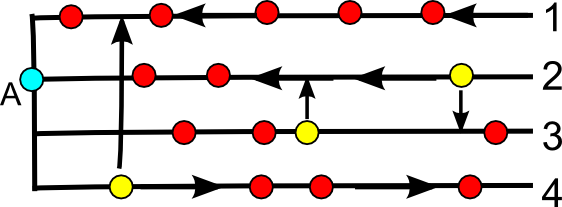
\includegraphics[width=.5\textwidth]{gen_pdmppic.png}
\caption{\textbf{A PDMP on four species}.  Particles travel on four separate copies of $\mathbb{R}^+$.  Velocity directions are represented by horizontal arrows, with species 3 having zero velocity. A boundary event occurs when a particle (labelled by ``A") hits the origin.  Here, three particles  are then randomly selected ($K^{(2)} = 3$), and reassigned  to different species by predetermined reassignments (given by vertical arrows). In this example, $R_{41}^{(2)} = 1, R_{32}^{(2)} = 2$, and $R_{23}^{(2)} = 3$. }
\label{pdmppic}
\end{centering}

\end{figure}  





 













\section{The $k$-species model in a PDMP framework}\label{itsapdmp}
\subsection{PDMP formulation of  the $k$-species model} 
We now show the $k$-species model is a specific class of PDMP, as outlined in Section \ref{pdmpgenerator}. Define the possible listings of species
\begin{equation}
 \mathcal S= \bigcup_{i \in \mathbb N}\{1, \dots, M\}^{i},
 \end{equation}   For a species index $\mathbf { s} = (s_{1},\dots, s_{|\mathbf s|})$ of length $|\mathbf s|$, a state has the form $(x_1, \dots, x_{|\mathbf s|})\in (\mathbb{R}^+)^{|\mathbf s|}$. 
 We write the state space of particles as    
\begin{equation}
E =\coprod_{\vec s \in \mathcal S } ((\mathbb{R}^+)^{|\mathbf s|})_\mathbf s = \left\{(\textbf s,(x_{1}, \dots, x_{|\mathbf s|}):\textbf s \in \mathcal S, (x_{1}, \dots, x_{|\mathbf s|})\in \mathbb{(R}^+)^{|\mathbf s|}\right\}.  
\end{equation}
A state $\textbf{x} \in E$ can thus be described as an element of  $(\mathbb{R}^+)^{|\mathbf s|}\times \mathbb N^{|\mathbf s|}$, where we will write
\begin{equation}
\textbf{x} = \left((s_{1},x_1), \dots, (s_{|\mathbf s|},x_{|\mathbf s|})\right).
\end{equation} 
Vector fields will then be represented by  
\begin{equation}
\mathcal X_{\vec s} = \sum_{i = 1}^{N} v_{s_i}(x_i)\frac{\partial}{\partial x_i}.
\end{equation}


   The exit boundary of $\Gamma^*\subset E$ consists of  particles that hit the origin.
\begin{equation}
\Gamma^* = \{\mathbf x\in E| \hbox{there exists }  (s_i,x_i) \hbox{ where }   x_i = 0, s_i\le M_-\} 
\end{equation}

To describe the transition kernel $Q$, we denote the set of states that  $\textbf{x} \in \Gamma^*$ can jump to as $E_b(\textbf{x})$.  This set of events is finite, and have well-defined (albeit, tedious to calculate) probabilities of a reassignment for a state $\textbf{x}$ jumping to $\textbf{x}_b$, denoted $p_{b}(\textbf{x}_b, \textbf{x})$.  These probabilities are uniquely determined from the weights $w^{(l)}_k$, numbers $|L_i|$, and reassignments $R_{ij}^{(l)}$, and therefore are functions of the current state $\textbf{x}$.   Similarly, we can define jump probabilities for interior events as $p_{int}(\textbf{x}_{int},\textbf{x}) $. Here, $\textbf{x}_{int} \in E_{int}(\textbf{x})$ denotes the set of possible states that $\textbf{x}\in E$ can jump to.  Thus, we can define
\begin{equation}
Q(y,\textbf{x}) = \begin{cases}p_{b}(y,\textbf{x}) & \textbf{x} \in \Gamma^*, y\in E_b(\textbf{x}) \\
p_{int}(y,\textbf{x}) & \textbf{x} \in E, y \in E_{int}(\textbf{x})   \\
0 & \hbox{otherwise}. 
\end{cases}
\end{equation}
Since each particle has a Poisson clock of parameter $\beta$, the distribution $Y$ of the first time that a clock rings follows the distribution 
\begin{equation}
Y \sim \min_{1\le i\le N} Poisson(\beta) = Poisson(N\beta).
\end{equation}
Thus $\lambda(\textbf{x}): E \rightarrow \mathbb{R}$ takes the form
\begin{equation}
\lambda(\textbf{x}) = \beta |\mathbf s|.
\end{equation}
With this, we now have a well defined PDMP which describes particle reassignments among different species.

\subsection{The main theorem}


For $\textbf{x} \in E$, we define empirical measures $\mu^N_i(\textbf{x}) \in \mathcal M(\mathbb{R}^+)$ by
\begin{equation}
\mu_i^N(\textbf{x}) = \sum_{x_j \in L_i} \frac{\delta_{x_j}}{N}, \quad i = 1,\dots, M.
\end{equation}
For a process $X(t)$, we will often write $\mu_i^N(X(t)):=\mu_i^N(t)$.
For the class of test functions
\begin{equation}
\mathcal C = \{\phi\in C^1(\mathbb{R}^+)\cap C_b(\mathbb{R}^+) : \phi(0) = 0, \phi' \in C_b(\mathbb{R}^+)\},
\end{equation} 
we can pair empirical measures with test functions through integration:
\begin{equation}
\langle \phi, \mu_i^N \rangle = \int_{\mathbb{R}^+} \phi(x)\mu_i^N(dx) = \sum_{x_j \in S_i} \frac{\phi(x_j)}{N}, \quad \phi \in \mathcal C, i = 1, \dots, M,
\end{equation}
where $S_i$ denotes the support of particles in species $i$, for $i = 1,\dots, M$ .

Our main result shows that empirical measures $\mu^N_k(t)$ approximate a weak solution to a transport equation, with a source term given by the flux of particles from both interior and boundary events. These measures are simplest to describe  when viewed as smooth limits $\mu_k(t)$  of particle densities $\mu_k^N(t)$ as $N\rightarrow \infty$ of the form
\begin{equation}
u_k(x,t)dx = \mu_{k}(t)(dx),     \quad k = 1, \dots, M.  
\end{equation}
We also denote the total numbers
\begin{eqnarray}
\lefteqn{g_k(t)= \int_0^\infty u_k(x,t) dx,}\\
&& G(s) = \sum_{i = 1}^M g_i(t), \quad G^{int}(s) = \sum_{i = 1}^Mw_k^{int}g_k(t), \quad k = 1, \dots, M. \nonumber 
 \end{eqnarray}
and species selection weight fractions for boundary events
\begin{equation}\label{sswf}
W_j^{(l)}(t)= \frac{w^{(l)}_j}{\sum w^{(l)}_m g_m(t)} \quad l = 1,\dots, M_{-} \quad j = 1,\dots, M.
\end{equation}
The limiting number densities $u_k(x,t)$, $k = 1, \dots, M$, will satisfy the following system of PDE,
 \begin{eqnarray} 
  \lefteqn{\partial_t u_k(x,t)+\partial_{x}(v_k(x)u_{k}(x,t))=  \phantom{u_j(x,t)\mathbf{1}_{R^{(l)}_{ij}}
-K^{(l)}W_k^{(l)}(t)u_k(x,t)}}\label{smooth1}\\
 && \sum_{l = 1}^{M_-}u_l(0,t)v_{l}(0)\left[\sum_{i = 1}^{M}\sum_{j= 1}^{K^{(l)}} W_i^{(l)}(t)u_i(x,t)\mathbf{1}_{R^{(l)}_{ij}=k}
-K^{(l)}W_k^{(l)}(t)u_k(x,t)\right]\label{smooth2}\\ 
&&+\frac{\beta G(t)}{G^{int}(t)}\left( \sum_{i = 1}^{M}\sum_{j= 1}^{K^{int}} w^{int} _iu_{i}(x,t)\mathbf{1}_{R^{int}_{ij} = k}-K^{int}w^{int}_ku_{k}(x,t)
 \right)\label{smooth3}
 \end{eqnarray}
 with initial conditions 
 \begin{equation}
u_k(x,0) = u_{k}^0(x), \quad k = 1,\dots, M.
\end{equation}

  The first line (\ref{smooth1}) describes advection of species densities under the velocity field $v_k$.  The next line (\ref{smooth2}) describes the  the growth and loss of species $k$ due to boundary events. The first term of  (\ref{smooth2}) describes rates of incoming particles to species $k$.  This is reflected in the use of indicator functions, where  $R_{ij}^{(l)}$ determine species to which particles are reassigned. The next term describes loss from species $k$ to other species. This does not depend on reassignment, so we should expect no $R_{ij}^{(l)}$ terms.      The final line (\ref{smooth3}) contain source terms due to interior events.  These terms do not depend on $u_l(0,t)$, as the rate of interior events is only dependent on total total numbers $g_i(t)$.

  Our main theorem describes the convergence  of empirical measures to a weak form of the limiting PDE (\ref{smooth1})-(\ref{smooth3}), under the assumption of convergence of initial empirical measures to a nonatomic measure. 

\begin{theorem}\label{pdmpproof}
Let $\mu_k^0 \in\mathcal M(\mathbb{R}^+)$ be nonatomic. Suppose that we have weak convergence of initial empirical measures $\mu_k^{0,N} \rightarrow \mu_k^0$ as $N\rightarrow \infty$ in $\mathcal M(\mathbb{R}^+)$.  Then 
\begin{enumerate}
\item There exists a  time $T_e>0$ such that the   $\mu_k^N(t)$ converge to  limits $\mu_k(t)$ along a subsequence under the Skorohod topology $\mathbb D([0,T_e],\mathcal M(\mathbb{R}^+))$.
\item The empirical losses $F_l^N(t)$ of the total number deleted in species $l$  converge to continuous cumulative distribution functions $F_l(t)$ along a subsequence in the mean $L^\infty$ metric:
\begin{equation}
\lim_{N\rightarrow \infty}\mathbb E\left[\sup_{s\le T_e}|F_l^{N}(s)-F_{l}(s)|\right  ]= 0.
\end{equation}
\item The  $\mu_k(t)$ satisfy the following limiting equations for all
$\phi \in \mathcal C:$
\begin{eqnarray}\label{limeq}
\lefteqn{\langle \mu_k(t), \phi\rangle  - \langle \mu_k^0, \phi\rangle+\int_0^t\langle \mu_k(s), \phi' v_k \rangle=}\\ 
&&\sum_{l = 1}^{M_-}\mathlarger{\int_0^t} \left[\sum_{i = 1}^{M}\sum_{j= 1}^{K^{(l)}}W_i^{(l)}(s)\langle \mu_i(s), \phi\rangle\mathbf{1}_{R^{(l)}_{ij} = k}  -K^{(l)}W_k^{(l)}(s)\langle \mu_k(s), \phi\rangle\right ] \, dF_{l}(s)\nonumber\\  
&& +\mathlarger{\int_0^t}\frac{\beta G(s)}{G^{int}(s)}\left[-K^{int}w^{int}_k\langle \mu_k(s), \phi \rangle +\sum_{i = 1}^{M}\sum_{j= 1}^{K^{int}} w^{int}_i\ \langle \mu_i(s), \phi \rangle\mathbf{1}_{R^{int}_{ij} = k}\right]ds, \nonumber
\end{eqnarray}
for $k = 1, \dots, M$.


\end{enumerate}
 


\end{theorem} 
\begin{rem}\label{unifremark}
Since individual jumps of the prelimit PDMP converge to zero as $N\rightarrow \infty$, the limiting functions $\langle \mu_k(t), \phi\rangle, k = 1, \dots, M$ are continuous in $t$, meaning that empirical measures also converge in the local uniform metric (see Prop. 1.17 in Chapter VI of \cite{jac87}).    
\end{rem}
As we will see in Section \ref{bounddim}, the functions $F_l(s)$ can be seen as an integral of the trace of measures $\mu_l(s)$ occurring at the boundary. In fact, for continuous solutions, we will show that $dF_l(s) = v_l(0)u(0,s)ds$. 

We also state a well-posedness theorem for $L^1\cap L^\infty$ initial data, which is proved in Section \ref{uniquesect}.

\begin{deef}
For $k = 1, \dots, M$, let $u_{k}(x,t) \in C([0,T_e],L^1\cap L^\infty(\mathbb{R}^+,\mathbb{R}^+))$. We call $u_{k}(x,t)$ a \textbf{weak solution in $L^1\cap L^\infty(\mathbb{R}^+,\mathbb{R}^+)$} of  (\ref{smooth1}) with initial conditions $u_k^0(x) \in L^1\cap L^\infty(\mathbb{R}^+,\mathbb{R}^+),$ if for all $\phi\in \mathcal C$, there exist $\mu_k(t)$, $t\in [0,T_e]$, that satisfy (\ref{limeq}), with $\mu_k(t)(dx) = u_{k}(x,t)dx$, and $\mu_k(0)(dx) = u_{k}^0(x)dx$.   
\end{deef}

\begin{theorem}\label{wellposed} For $k = 1, \dots, M$,  there exists a unique   weak solution $u_{k}(x,t)$ in $L^1\cap L^\infty(\mathbb{R}^+,\mathbb{R}^+)$ of  (\ref{smooth1}) with initial conditions $u_k^0(x) \in L^1\cap L^\infty(\mathbb{R}^+,\mathbb{R}^+)$.
\end{theorem}

\begin{rem}
Theorem \ref{wellposed} should not be mistaken as stating that empirical measures with $L^1\cap L^\infty$ initial data converge in the uniform metric to a unique $L^1\cap L^\infty$ solution of (\ref{limeq}). Rather, in the class of all possible solutions, there is one, and only one, solution that is in $C([0,T_e],L^1\cap L^\infty(\mathbb R^+))$    \end{rem}
 
Well-posedness of  (\ref{limeq}) for $L^1$ data is discussed in Section \ref{uniquesect}.  




\subsection{Method of proof}


As a Markov process, the PDMP $X(t)$has an associated infinitesimal generator and martingale, given by \ref{generator} and \ref{martingale}, along with Rolski's conditions for membership in the domain $\mathcal D(\mathcal A))$, as shown in Theorem \ref{fourcond}. The method for proving Theorem \ref{pdmpproof} relies on   constructing  martingale equations that are approximations of (\ref{limeq}).  Unfortunately, the  domain of functionals for the infinitesimal generator of $X(t)$ is very limited. A na\"ive approach for proving Theorem \ref{pdmpproof} might take empirical pairing functionals \begin{equation}
f^\phi_k(\textbf{x}) = \langle \phi(x),\mu_k^N \rangle, \quad k = 1, \dots, M.
\end{equation}
 This, however, does not satisfy the boundary condition (3) of Theorem \ref{fourcond} for any nontrivial class of test functions. To see this, notice that if we restrict attention to a particular species $L_k$, then we shouldn't expect $\Delta f^\phi_k(\mathbf x)$ to retain its expected value when  a particle is deleted from or added to  $L_k$. For an example, refer to Fig. \ref{genex}. At the boundary event shown, for $\mathbb{E}[\Delta f^\phi_1(\mathbf x)]= 0$ we need $\phi(0) = \langle \mu^N_2,\phi\rangle$.  But  $\mu_2^N$ will change in time, so imposing such a restriction for any non-zero $\phi$ is unreasonable. 
\begin{figure}
\begin{centering}
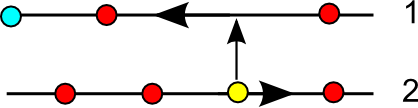
\includegraphics[width=.5\textwidth]{generatorexample.png}
\caption{\textbf{A PDMP on two species.} In this case $K^{(1)} = 1$, with $R^{(1)}_{21}= 1$. }  \label{genex}     
\end{centering}
\end{figure}

To allow for functionals which track empirical measures on $L_k$, in Section \ref{extension} we will construct an extended PDMP $\tilde X(t)$ from $X(t)$ with added dimensions that track boundary events. We can then select  functionals $F^\phi_k(\tilde {\textbf x})$ in the domain   $\mathcal D(\tilde {\mathcal A})$ of the extended generator $\tilde{\mathcal A}$.  These functionals satisfy condition (3) by adding a correction term to $f^\phi_k(\textbf{x})$, dependent on the extra dimensions in $\tilde{\textbf{x}}$.

For each species $k$, we will use $F^\phi_k(\tilde {\textbf x})$ to construct the martingales from (\ref{martingale}). These martingales involve empirical pairings  $\langle \mu^N,\phi\rangle$ and terms $B_{i,j}^{\phi,N}(t)$, which roughly describe total occurrences of boundary events.   We show the limit of these equations approaches (\ref{limeq}) as $N \rightarrow \infty$.  To do so, we first  show the martingale term $M_\phi^{k,N}(t)$ converges to zero in the local uniform metric, a consequence of Doob's theorem. The most technical part  involves the tightness of empirical pairings .  As in Chapter 2, we will use the Theorems \ref{Ald} and \ref{Cap} to show tightness of $\mu_k$.
 
Finally, we focus our attention on the terms $B_{i,j}^{\phi,N}(t)$. Using a law of large numbers type argument, we will show these  terms  converge in the local uniform metric to terms involving $\langle \mu_k, \phi\rangle$ and $F_k(t)$. 











\section{The extended PDMP $\tilde X^{N}(t)$}\label{extension}


 To address condition (3) of Theorem \ref{fourcond}, let us denote $\tau_i^{j,k}$ as the $i^{th}$ time that a boundary event reassigns a particle from $L_j$ to $L_k$. Note that $\tau_i^{j,k}$ may equal $\tau_m^{j,k}$ when $m>i$, since boundary events can reassign more than one particle.  Ordering of $\tau_i^{j,k}$  when several particles are simultaneously reassigned from $L_j$ to $L_k$  is done with respect to the same ordering used to determine reassignments $R_{jk}^{(l)}$.   Suppose we have $\kappa_{j,k}^N(t)$ particles $(x_1, \dots, x_{\kappa_{j,k}^N(t)})$ that have been reassigned from $L_j$ to $L_k$, at times  $\tau_i^{j,k}$. We now define \textbf{boundary variables} that track jumps from boundary events as 
\begin{equation}
B_{j,k}^{\phi,N}(t) = \sum_{i = 1}^{\kappa_{j,k}^N(t)} \frac{\phi(x_i)}{N} \quad \phi \in \mathcal C.
\end{equation}
  

 
We now define the extended PDMP $\tilde X^{N}(t)$ which tracks jumps occurring in $X^{N}(t)$.   Formally, we can write the extended state space as 
\begin{equation}
\tilde E = \coprod_{\vec s \in K } (\mathbb{R}^{|\mathbf s|+M^2}_+)_\mathbf s = \left\{(\mathbf s,\tilde{\mathbf x}):\mathbf s \in K, \tilde{\mathbf x} \in \mathbb{R}_+^{|\mathbf s| + M^2}\right\}. 
\end{equation}
A state $\tilde {\textbf{x}} \in \tilde E$ can be written as 
\begin{equation}
\tilde {\textbf{x}} = \left(x_1, \dots, x_{|\mathbf s|},b_{1}^1, \dots b_1^M, \dots, b_{M_-}^1, \dots, b_{M_-}^M\right).
\end{equation} 
The quantities $b_i^j$ are a means of recording the number and type of boundary events which occur.  We impose that boundary variables have no drift in $\tilde E$, which means that for vector fields in $\tilde{ \mathcal X}$, we let $\tilde{\mathcal X}_{\vec s}= \mathcal X_{\vec s}$, and define the exit boundary as
\begin{equation}
\tilde \Gamma^*(\tilde {\textbf{x}}) = \left\{(y, b_1^1, \dots, b_{M_-}^M)| y \in \Gamma^*\right \}.
\end{equation}
The main difference between $\tilde{\textbf{x}}$ and $\textbf{x}$ is seen in the extended transition kernel $\tilde Q$. For $\tilde {\textbf{x}}\in \tilde E$, the set of possible states  $\tilde E_{int}(\tilde {\textbf{x}})$ that $\tilde {\textbf{x}}$ may jump to from interior events is simply the the set $E_{int}(\textbf{x})$ with added unchanged boundary variables:
\begin{equation}
\tilde E_{int}(\tilde {\textbf{x}})  = \left\{(y, b_1^1,\dots, b_{M_-}^M)| y \in E_{int}(\textbf{x})\right\}.
\end{equation}
For $\tilde {\textbf{x}} \in \tilde \Gamma^*(\tilde E)$, however, boundary variables will increase, corresponding to the types of boundary events that occur at $\tilde{\mathbf x}$. Suppose a boundary event, triggered from a particle hitting the origin of $L_l$, selects particles $x_1, \dots, x_{K^{(l)}}$. We then define the new possible states of $\tilde {\textbf{x}}$ as 
\begin{equation}
\tilde E_b(\tilde {\textbf{x}})  = \left\{(y, \tilde b_1^1,\dots,\tilde  b_{M_-}^M)| y \in E_b(\textbf{x})\right\},
\end{equation}
where boundary variables change as 
\begin{equation}
\tilde b_i^j =  b_i^j+ \sum_{x_k\in L_i}\sum_{j = 1}^M \frac{\phi (x_k)}{N}\textbf{1}_{R^{(l)}_{ik} =j}, \quad i,j = 1, \dots, M . \end{equation}
Thus, boundary variables add the sum of quantities $\phi(x_k)$ to $b_i^j$, where $x_k$ is reassigned from $L_i$ to $L_j$.
We can then express the extended transition probability as  
\begin{equation}
\tilde Q(y,\tilde {\textbf{x}}) = \begin{cases}p_{b}(y,\tilde {\textbf{x}}) & \tilde {\textbf{x}} \in \tilde \Gamma^*, y\in \tilde E_b(\textbf{x}) \\
p_{i}(y,\tilde {\textbf{x}}) & \tilde {\textbf{x}} \in E, y \in \tilde E_{int}(\textbf{x})   \\
0 & otherwise. 
\end{cases}
\end{equation}
We thus have a well defined PDMP $\tilde X(t)$ determined from $\tilde E, \tilde{\mathcal X},$ and $ \tilde Q$. From here it is not hard to see that 
\begin{equation}
\tilde X(t) = \left(x_1(t), \dots, x_{|\mathbf s|}(t),B_{1,1}^{\phi,N}(t), \dots B_{1,M}^{\phi,N}(t), \dots, B_{M_-,1}^{\phi, N}(t), \dots, B_{M_-,M}^{\phi,N}(t)\right)
\end{equation} 


With the parameters $B_{j,k}^{\phi,N}(t)$ at our disposal, we may now define functionals
\begin{equation}
F^{\phi,N}_k(\tilde X(t)) = \sum_{x(t)\in L_k} \frac{\phi(x(t))}{N}+\sum_{j= 1}^M B_{j,k}^{\phi,N}(t)-B_{k,j}^{\phi,N}(t) , \quad k = 1, \dots, M. 
\end{equation}
\section{Reassignment bounds and martingale equations}
To show that  $F^{\phi,N}_k$ is a valid functional in the domain of the infinitesimal generator $\tilde{\mathcal{A}}$, we give a simple bound for jumps which will be utilized throughout this paper.  Denote the maximum number of reassigned particles at a critical event by 
\begin{equation}
K = K^{int} \vee \max_i K^{(i)}.
\end{equation}


\begin{lem}\label{jumpbound}  The number of particle interior events $m_{int}^N$ and  reassignments $\kappa^N(t)$ has bounds
\begin{enumerate}
\item (\textbf{Expectation for fixed} $N$) For any $N \in \mathbb N$, we have 
\begin{equation}
\mathbb{E} [m^N_{int}(t)]\le \beta Nt,
\end{equation}  and
\begin{equation}
\mathbb{E} [\kappa^N(t)]\le KN(1+\beta t).
\end{equation}

\item 
(\textbf{Law of large numbers bound})  
\begin{equation}
\limsup_{N\rightarrow \infty} \frac{m^N_{int}(t)}{N}\le \beta t    \quad a.s., 
\end{equation} 
and
\begin{equation}
\limsup_{N\rightarrow \infty} \frac{\kappa^N(t)}{N}\le K(1+\beta t)    \quad a.s.. 
\end{equation}


\end{enumerate}  
\end{lem}
\begin{proof} Clearly, the number of boundary events is bounded by the initial number of particles $N$.   The expected rate of interior events $m_{int}^N(t)$ can be bounded by the Poisson parameter $\beta(X^N(t)) = \beta (N(t))\le \beta N$.    The expected number of jumps up to time $t$ is thus bounded by $\beta Nt$, which proves (1).  

For part (2), we note that a Poisson process $P_\gamma(t)$ of intensity $\gamma$ at time $t$ satisfies the scaling argument
\begin{equation}
P_\gamma(t) \sim P_{a\gamma}(t/a) \quad a>0.
\end{equation}
It then follows  from the law of large numbers for Poisson processes,
\begin{equation}
\frac{P_\gamma(t)}{t} \rightarrow \gamma \quad a.s. \hbox{ as } t \rightarrow \infty,
\end{equation}
 that we can obtain  
\begin{eqnarray} 
\mathbb P(\limsup_{N \rightarrow \infty}\frac{m_{int}^N(t)}{N}>\beta t) \le \mathbb{P}\left(\limsup_{N \rightarrow \infty}\frac{P_{N\beta}(t)}{N} >\beta t\right)\\
= \mathbb{P}\left(\limsup_{N \rightarrow \infty}\frac{P_{\beta}(Nt)}{Nt}t > \beta t\right) = 0, \nonumber \end{eqnarray}    
which proves part (2).   
\end{proof}

\begin{theorem}\label{gencalcs}
For the domain of the infinitesimal generator $\mathcal D(\tilde {\mathcal A})$ corresponding to $\tilde x$, we have $F^{\phi,N}_k \in \mathcal D(\tilde {\mathcal A})$, for $k = 1,\dots, M$. 
\end{theorem}

\begin{proof} We need to show the four conditions of Theorem \ref{fourcond} hold for $F^{\phi,N}_k$.  Conditions (1) and (2) are clear, since particles in $\tilde E$ transport along a continuous flow, and $\phi \in C^1(\mathbb{R}^+)$.

For condition (4), we need to make estimates on the frequency of jumps in $\tilde E$.  We first note 

\begin{equation}
\mathbb E\left[B_{j,k}^{\phi,N}(t)\right] \le \mathbb E[\kappa^N(t)]\frac{\|\phi\|_\infty}{N}.  
\end{equation}
Let us define the the $m^N(t)$ jump times before time $t$ as $\tau_1, \dots, \tau_{m^N(t)}$. Then from Lemma \ref{jumpbound},
\begin{eqnarray}
\mathbb{E}\left[\sum_{i = 1}^{m^N(t)} |F_k^{\phi,N}(\tilde X(
\tau_i)-F_k^{\phi,N}(\tilde X(\tau_{i-1}))|\right]  \\
\le \mathbb{E}\Big [\sum_{i = 1}^{m^N(t)}|\langle \mu^N_k(\tau_i),\phi\rangle-\langle \mu^N_k(\tau_{i-1}),\phi\rangle|\nonumber\\+\sum_{j = 1}^M|B_{j,k}^{\phi,N}(\tau_i)-B_{k,j}^{\phi,N}(\tau_i)+ B_{j,k}^{\phi,N}(\tau_{i-1})-B_{k,j}^{\phi,N}(\tau_{i-1})|  \Big]\nonumber  \\
\le \frac{4M}N\mathbb{E}[\kappa^N(t)]\le\frac{4MK}N(\beta tN+N) \nonumber \\
< \infty.  \nonumber
\end{eqnarray}
The nontrivial part to show is the boundary condition (3).
 Note that for $X(\tau^-) \in \Gamma^*$, 
  \begin{eqnarray}
 \int_E F_k^{\phi,N}(y)-F(X(t^-)) Q(dy,X(t^-)) = \mathbb E(\Delta F_k^{\phi,N}(X(t)))\\
 =\mathbb E\left[\Delta \langle \mu_k^N(t), \phi \rangle \right]+\sum_j\mathbb E\left[\Delta B_{j,k}^{\phi,N}(t) -\Delta B_{k,j}^{\phi,N}(t) \right].\nonumber 
\end{eqnarray}
Assume that a  boundary event at jumping time $\tau$ occurs from a particle hitting the origin in $L_l$, and randomly selects $K^{(l)}$ particles $(x_1, \dots, x_{K^{(l)}})$.  Then we have the expected change in empirical measure as a sum of the averages resulting from particles leaving and entering $L_k$: 
\begin{align}  
&\mathbb E[\Delta \langle \mu_k^N(\tau, \phi) \rangle ] = K^{(l)}p_k^{(l)}(\tau)\cdot\mathbb{E}\left[\frac{\phi(x_1)}{N}|x_1 \in L_k \right]\\&+\sum_{i= 1}^{M}\sum_{ j = 1}^{K^{(l)}}p_i^{(l)}(\tau) \cdot\mathbb{E}\left[\frac{\phi(x_1)}{N}|x_1 \in L_i \right]\mathbf{1}_{R^{(l)}_{ij} = k}\nonumber\\
&=  - \frac{K^{(l)}w^{(l)}_k}{N^{l}} \langle \mu_k^N(\tau), \phi \rangle +\sum_{i= 1}^{M}\sum_{ j = 1}^{K^{(l)}} w^{(l)}_i\frac{\langle \mu_i^N(\tau), \phi \rangle}{N^{(l)}}\mathbf{1}_{R^{(l)}_{ij} = k}. \nonumber 
\end{align}
However, we see that for jumps in the boundary variables,
by similar calculations, at a boundary jumping time $\tau$ 
\begin{equation}
\sum_j\mathbb E\left[\Delta B_{j,k}^{\phi,N}(\tau)\right] = \sum_{i = 1}^{M} \sum_{m= 1}^{K^{(l)}} w^{(l)}_i\frac{\langle \mu_i^N(\tau), \phi \rangle}{N^{(l)}}\mathbf{1}_{R^{(l)}_{im} = k}
\end{equation}
for expectations of particles entering species $k$, and   
\begin{align}
\sum_j\mathbb E\left[\Delta B_{k,j}^{\phi,N}(\tau)\right]  &=  -K^{(l)}p_k^{(l)}(\tau)\mathbb{E}\left[\frac{\phi(x_1)}{N}|x_1 \in L_k\right] \\ 
&= \frac{K^{(l)}w^{(l)}_k}{N_{l}} \langle \mu_k^N(\tau), \phi \rangle \nonumber  \end{align}
for particles leaving species $k$.
\end{proof}
  In the following, define the empirical total number as
  \begin{equation}
  G^N(s)=\sum_{k = 1}^M \langle \mu_k^N(\tau), 1 \rangle, \quad G^{int,N}(s)=\sum_{k = 1}^M w_k^{int}\langle \mu_k^N(\tau), 1 \rangle 
  \end{equation}
  To each $F_k^{\phi,N}$, we can now construct the following martingale.  

\begin{theorem} For $k \in \{1, \dots, M\}$, the quantity 
\begin{align}\label{mgaleeqn}
&M_k^{\phi,N}(t) = \langle \mu_k^N(t), \phi\rangle- \langle \mu_k^N(0), \phi\rangle+\\
&\sum_{j= 1}^M B_{j,k}^{\phi,N}(t)-B_{k,j}^{\phi,N}(t) -\int_0^t \langle \mu_k^N(s), \phi' v_k \rangle +\nonumber \\
&\frac{\beta G^N(s)}{G^{int,N}(s)} \left[K^{int}w^{int}_k \langle \mu_k^N(s),\phi\rangle\frac{}{}-\sum_{i = 1}^{M}\sum_{j = 1}^{K^{int}}\  w^{int}_i \langle \mu_i^N(s),\phi\rangle\mathbf{1}_{R^{(l)}_{ij} = k}\right]ds \nonumber  
\end{align}
is a martingale.
\end{theorem}

\begin{proof}
The vector field $\tilde{\mathcal X}$ acts only on the first $N$ coordinates of $\tilde x$, and satisfies
\begin{eqnarray}
 \tilde{\mathcal X}(F_k^{\phi,N}(\tilde x)) = \sum_{i = 1}^{N} \sum_{x_i \in L_k}v_{s_i}(x_i)\frac{\partial}{\partial x_i}\frac{\phi(x_i)}{N} = \sum_{x_i \in L_k} v_k(x_i)\frac{\phi'(x_i)}{N} \\
 = \langle \mu_k^N, \phi' v_k \rangle \nonumber 
 \end{eqnarray}
Using equation (\ref{generator}), our formula for the extended generator is then
\begin{align}\label{genequa}
\tilde{\mathcal A}(F_k^{\phi, N}(\tilde x))&  \\ &=\langle \mu_k^N, \phi' v_k \rangle -\beta(\tilde x)\int_E (F_k^{\phi, N}(y)-F_k^{\phi, N }(\tilde x))Q(dy;\tilde x)) \nonumber\\
&= \langle \mu_k^N, \phi' v_k \rangle -\beta N \mathbb{E}\left[\Delta(F_k^{\phi, N}(\tilde x))\right].\nonumber 
\end{align}  
The calculation of the change of the functional over interior events is similar to Theorem \ref{gencalcs}:
\begin{align}\label{intfunct}
 &\mathbb{E}\left(\Delta(F_k^{\phi, N}(\tilde x))\right)=  \frac{K^{int}p^{int}_k }{|L_{k}|} \langle\mu_k^N,\phi\rangle-\sum_{i = 1}^{M}\sum_{j=1}^{K^{int}}  \frac{p^{int}_i }{|L_{i}|}\langle \mu_i^N,\phi\rangle\mathbf{1}_{R^{(l)}_{ij} = k}\\ 
&= \frac{1}{G^{int,N}(s)}\left[K^{int}w^{int}_k \langle \mu_k^N(s),\phi\rangle\frac{}{}-\sum_{i = 1}^{M}\sum_{j = 1}^{K^{int}}\  w^{int}_i \langle \mu_i^N(s),\phi\rangle\mathbf{1}_{R^{(l)}_{ij} = k}\right]. \nonumber 
\end{align}

Combining terms, we see the martingale $M_k^{\phi,N}(t)$ defined from equation (\ref{martingale}) then coincides with (\ref{mgaleeqn}).  
\end{proof}

We now uniformly bound the martingale $M^{\phi,N}_k(t)$, which will decay to zero in the mean $L^\infty$ metric.  
\begin{theorem} For $t<T_e$ we have 
\begin{equation}
\mathbb{E}[\sup_{s \in [0,t]}(M_k^{\phi,N}(s))] \le \frac{(4M+2)K\|\phi\|_\infty\sqrt{1+\beta t}}{\sqrt N},
\end{equation}
\end{theorem}
\begin{proof}

We bound jumps in $M^{\phi,N}_k(t)$ by noting that at most $K$ particles are either reassigned in a critical event: 

\begin{equation}
|\Delta M_k^{\phi,N}(t) |= |\Delta\langle \mu^{N}_k(t),\phi\rangle|+|\Delta (\sum_{j = 1}^M B_{j,k}^{\phi,N}(t)+B_{k,j}^{\phi,N}(t))|\ \le \frac{(2M+1)K\|\phi\|_\infty}N. \end{equation}

It then follows that, from Lemma \ref{jumpbound}, that
\begin{align}\label{martinq}
&\mathbb E[M_k^{\phi,N}(t)^2] = \mathbb{E}\left [\sum_{i = 1}^{m_N(t)}\Delta M_k^{\phi,N}(\tau_i)^2\right ]\\
&\le\frac{(2M+1)^2K^2\|\phi\|^2_\infty}{N^2} \mathbb{E}[m_N(t)]\le \frac{(2M+1)^2K^2\|\phi\|^2_\infty(1+\beta t)}{N}. \nonumber   
\end{align}

 

We now use Doob's inequality to obtain
\begin{equation}\label{moarmartinq}
\mathbb{E}\left[\sup_{s \le t}|M_k^{\phi,N}(s)|\right]^2 \le \mathbb E\left[\sup_{s \le t} M_k^{\phi,N}(s)^2\right] \le 4\mathbb E[M_k^{\phi,N}(t)^2].
\end{equation}
The result follows from applying (\ref{martinq}) to (\ref{moarmartinq}).
\end{proof}

\section{Existence of limiting measures}\label{cogito}

We base the existence interval $T_e>0$ off of when species will have positive total numbers almost surely.  The following lemma ensures that the transition probabilities, and subsequently the kinetic equations (\ref{limeq}), are well defined. The technical details of the the following lemma will be utilized in Lemma \ref{geometric} in determining tightness of empirical measures. The existence time $T_e$ will eventually be extended to a reasonable time where the solution is well defined as long as each species has positive total particle number.    



\begin{lem}\label{mintime} There exists a time $T_e$ where, for all $k = 1, \dots, M$, and $0<t<T_e$, the following hold: \begin{enumerate}
\item (\textbf{Fraction loss of particles})  
\begin{equation}
\limsup_{N \rightarrow \infty} \sup_{0\le s\le t}g_k^N(s)>\frac 23g_k^0  \quad \hbox{ a.s.. }
\end{equation}
\item (\textbf{Total number of particles lost}) The quantity $H^{N}(t)=1-\sum_k g_k^N(t)$ is bounded by a fraction of the total number in each species:
\begin{equation}
\limsup_{N \rightarrow \infty}H^N(t)<\frac 1{3M^2K}\mu_k^0(\mathbb{R}^+) \quad \hbox{ for all } k \in \{1, \dots, M\} \quad \hbox{a.s..}
\end{equation}
\item
(\textbf{Fixed time bound}) The time $T_e$ is bounded by a constant determined from fixed parameters in $X$
\begin{equation}
T_e < \frac{\min_k g_k^0}{4\beta M^2K}.
\end{equation}
\end{enumerate}


\end{lem}

\begin{proof}
Denote the flow determined from vector fields $v_i$ at time $t$ on $L_i$ as $\varphi^i(t,x)$, with initial condition $\varphi^i(0,x) = x$. Regardless of the choice of reassignment of particles, the total particle number lost  from boundary deletions $H^{N}(t)$ can be crudely bounded by
\begin{equation}
\limsup_{N\rightarrow \infty} \sup_{0\le s\le t}H^N(s) \le \sum_{i = 1}^M \mu_k^0([0,a(t)]), 
\end{equation}
for all $N<\infty$, where $\varphi^i(s,a(t))>0$ for all $s\le t$ in $L_i$.  
Since the initial measures $\mu_k$ are nonatomic, we can choose $t_1$ such that
\begin{equation}\label{massbound}
\sum_{k = 1}^M \mu_k^0([0,a(t_1)])<\min_{1\le i \le M} \frac 1{3M^2 K}g_i^0  ,
\end{equation}
which shows part (2).  

We now show  part (1).  As noted in Lemma \ref{jumpbound}, the rate of interior events is bounded by $\beta N$, which means that the total particle total number lost through interior events $H_{int}^N(t)$ has the bound 
\begin{eqnarray}
\limsup_{N\rightarrow \infty}H_{int}^N(t_2^1) \le K\beta t_2^1\\<\min_{1\le i \le M} \frac 1{6}g_i^0 \quad a.s. \nonumber
\end{eqnarray}
for a sufficiently small $t_2^1>0$. Total loss from boundary events $H_{b}^N(t)$ satisfies the bound
\begin{eqnarray}
\limsup_{N\rightarrow \infty}H_{b}^N(t_2^2) \le\sum_{k = 1}^M \mu_k^0([0,a(t_2^{2})])\\<\min_{1\le i \le M} \frac 1{6}g_i^0, \nonumber
\end{eqnarray}  
for a sufficiently small $t_2^2>0$.  Letting $t_2 = t_2^1 \wedge t_2^2$ then shows part (1), and letting 
  
\begin{equation}
T_{e}=t_1\wedge t_2 \wedge \frac{1}{2\beta MK} 
\end{equation}
gives a positive time $T_e>0$ that satisfies all three conditions.
\end{proof}

In the following, denote the set of intervals $I_\delta$ of  length at most $\delta$ as
\begin{equation}
I_\delta = \{(a,b)\subset \mathbb{R}^+, b-a<\delta\}.
\end{equation}


Our method of proof shows  that the sequences $\mu_k^N(t)$ are approximately nonatomic with probability one as $N\rightarrow \infty$. We make this rigourous with the following definition.
\begin{deef}
 A sequence of random measure processes $\nu_t^n$ is \textbf{probabilistically approximately nonatomic} (p.a.n.a.) for time $T$ if for all $\eta > 0$,  \begin{equation}\label{paac}
 \lim_{\delta \rightarrow 0}\sup_{I \in I_\delta}\limsup_{n\rightarrow \infty} \sup_{t \in [0,T]}\mathbb P(\nu_t^n(I) >\eta) = 0 .
\end{equation}
\end{deef}
We will eventually demonstrate that the p.a.n.a. property is sufficient to show the Aldous conditions of Theorem \ref{Ald}. We aim to  express $\mu_k^N(t)$ by a decomposition of particles though their histories as different species. With this in mind, we have the following definition, which isolates subsets of particles in species $k$.

\begin{deef} A finite measure process $\mathscr A_k^N(t) \in \mathcal M(\mathbb{R}^+)\times [0,T_e]$   is a  \textbf{subparticle measure process of}  $\mu_k^N(t)$ if \begin{equation}
\mathscr A_{k}^N(t)= \sum_{\substack{x \in S^N(t) \\ }} \frac{\delta_{x}}{N}.
\end{equation}
for some support $S^{N}(t) \subset L_k$ satisfying $S^{N}(t) \subset S_k(X^{N}(t))$. \end{deef}



Given a subparticle measure process $\mathscr A_{j}^N(t)$ with support $S^{N}(t)$ , we can then define empirical measures of particles in $S^N(t)$ that jump from $L_j$ to $L_k$ and then flow on $v_k$ with no probability of jumping again. 


\begin{deef}
A \textbf{boundary running measure} $ \tilde{\mathscr A}_{j,k}^N(t) \in \mathcal M(\mathbb{R}^+)\times [0,T_e]$ of a subparticle measure process $\mathscr A_{j}^N(t)$ with support $S^{N}(t)$ is a measure of the form
\begin{equation}
\tilde{\mathscr A}_{j,k}^N(t) = \sum_{x\in U^k(s)}  \frac{\delta_{\varphi^k(\varphi^j(s, x), t-s)}}{N}
\end{equation}  
 with support
\begin{equation}
U^k(\tau) = \{x\in S^N(\tau^-) | \hbox{A boundary event at $\tau$ transfers $x$ to $L_k$}\}.
\end{equation}


We will denote the jump times of a running measure as $\tilde \tau_1,\dots, \tilde \tau_{\tilde m(t)}$, and the particles selected as $\tilde x_1, \dots, \tilde x_{\tilde m(t)}$, where $\tilde m(t)$ is the total number of such jumps.
\end{deef}
We can similarly define \textbf{interior running measures} $\tilde{\mathscr A}_{j,k}^{int,N}(t)$ for particles that jump from $L_j$ to $L_k$ due to interior events.  

\begin{theorem}\label{pacthm}  For $j,k = 1, \dots, M$ and  $t\in [0,T_e]$,  if the sequence of subparticle measure processes $R_j^N(t)$ is p.a.n.a., then so are running measures $\tilde R_{j,k}^{int,N}(t)$ and $\tilde R_{j,k}^{N}(t)$.
\end{theorem}

\begin{proof} 
Let $t \le T_e$.  
 Suppose a particle is chosen to transfer from $L_j$ to $L_k$ at time $s\le t$.  At a boundary event, after choosing a species $L_j$, particles are chosen uniformly on $L_j$ to reassign to another species. Thus, the (random) probability $q^N_s(I)$ of reassignment of a particle in the support of $R_j^N(s)$ in the correct interval at time $s$ before traveling to $I$ satisfies
\begin{equation}
q_s^N(I) = \frac{R_j^N(s)( \varphi^k(I, s-t))}{g_k^N(s)}.
\end{equation}
By the p.a.n.a. property of $R_j^N(t)$, for $\varepsilon>0$, there exists $\delta>0$ where for all $I \in I_\delta$
\begin{align}\label{probrightspec}
&\limsup_{N\rightarrow \infty} \sup_{s\le t} \mathbb P(q^N_s(I)>\varepsilon)\\
&\le \limsup_{N\rightarrow \infty} \sup_{s\le t}\mathbb P(R_j^N(s)( \varphi^k(I, s-t))> \frac{2g^0_k}{3}\varepsilon)<\varepsilon\nonumber
\end{align}
  The factor $2g_k^0/3$ arises from part 2 of Lemma \ref{mintime} , which bounds the total number of a particular species.
We now note that, from Markov's inequality, and part  2 of Lemma \ref{jumpbound}, for $I \in I_\delta$, 
 \begin{align}
 &\limsup_{N\rightarrow \infty} \sup_{t \in [0,T_e]}\mathbb P(\tilde R_{k,j}^{N}(t)(I) >\eta)\\
 &\limsup_{N\rightarrow \infty} \sup_{s \in [0,t]} \frac{\mathbb E\left[\tilde R_{j,k}^{N}(t)(I)\right]}{\eta}\le  \frac{K(1+\beta t)}{\eta}\limsup_{N \rightarrow \infty} \sup_{s\le t}\mathbb{E}(q_s^N(I)) \nonumber\\
 \nonumber \\  &\frac{K(1+\beta t)}{\eta}\limsup_{N \rightarrow \infty} \sup_{s\le t} \Big[\mathbb{E}(q_s^N(I)|q_s^N(I)>\varepsilon))\mathbb P(q_s^N(I)>\varepsilon)\nonumber\\&+\mathbb{E}(q_s^N(I)|q_s^N(I)>\varepsilon))\mathbb P(q_s^N(I)>\varepsilon)\Big]\nonumber\\&\le  \frac{K(1+\beta t)}{\eta} 2\varepsilon  \nonumber, 
\end{align}
As $\varepsilon$ is arbitrary, we may take $\delta\rightarrow 0$ to obtain our result. For interior particle submeasures, the proof is identical.   
\end{proof}

With probability one, a particle starting in $L_i$ at time $0$  visits a finite set of species  before arriving at its final destination at time $t$.  Suppose a particle $x(t)$ at time $\tau_k$ jumps from $L_{\sigma_k}$ to $L_{\sigma_{k+1}}$, for $k = 1, \dots, m$.  The locations of $x(t)$ can then be symbolically described through the following \textbf{path notation} $\mathcal P (x(t)) = (\Sigma(x(t)), \Theta(x(t)))$, with path location $\Sigma(x(t)) \in \{1, \dots , M\}^m, $ and jump description $\Theta(x(t)) \in \{\partial, I\}^{m-1}$.  Specifically, if $\Sigma(x(t))_i = \sigma_i$, and $\Sigma(x(t))_{i+1} = \sigma_{i+1}$, then $x(t)$ jumps from $L_{\sigma_i}$ to $L_{\sigma_{i+1}}$ at the $i^{th}$ jump time $\tau_{i}$. If $\Theta(x(t))_i = \partial$, then the $i^th$ jump is a boundary event at $\tau_i$, while $\Theta(x(t))_i = I$, denotes an interior event. The number of different species realized by a particle, or the length of a path, will be denoted $| \Sigma(x(t))|$.

We now define  \textbf{path measures} that keep track of particles that follow specific paths. for $\Sigma \in \{1, \dots , M\}^m$, denote
\begin{equation}
R_{\Sigma}(t)  = \{x(t) \in S_{\sigma_{|\Sigma|}}(t)|\Sigma (x(t)) = \Sigma \},
\end{equation}
and
\begin{equation}
\mu^N_{\Sigma}(t)= \sum_{x\in R_\Sigma(t)} \frac{\delta_x}{N}.
\end{equation}
It's straightforward to see that  $\mu^N_\Sigma(t)$ are subparticle measures. Path measures $\mu^N_\Sigma(t)$ with support $R_{\Sigma}(t)$ also have the following \textbf{no return property}: Suppose we track a specific particle $x(s) \in E$, with initial position $x_0 \in E$. If $x(t) \in R_{\Sigma}(t)$, and there exists $t'>t$ with $x(s) \in R_{\Sigma}(t')$, then $x(s) \in R_{\Sigma}(s)$ for $s \in [t,t']$. 

 The no return property ensures that a particle that is a member of $R_{\Sigma}(t)$ is not permitted to exit and reenter $L_k$. The importance of such a property will become apparent in the following theorem.  Denote the running measures of  $\mu^N_\Sigma(t)$ from $L_{\sigma_{|\Sigma|}}$ to $L_k$ as $\tilde \mu^N_{\Sigma,k}(t)$ and $\tilde \mu^{\beta,N}_{\Sigma,k}(t)$. We then have the following

\begin{theorem} \label{paacproof}
 $\mu^N_\Sigma(t), \tilde \mu^N_{\Sigma,k}(t)$,and $\tilde \mu^{\beta,N}_{\Sigma,k}(t)$ are p.a.n.a. for length $T_e$.
\end{theorem}

\begin{proof}We prove the theorem by induction on the path length $|\Sigma|$ .  For the base case,   $|\Sigma|= 1$ corresponds to particles which have not yet jumped from their initial distribution.  Thus the support of $\mu_\Sigma^N(t)$ is strictly contained in the support of the pullback measure $(\varphi^{\sigma_1})^*\mu^N(t)$, and is thus p.a.n.a., which implies that, from Theorem \ref{pacthm}, $\tilde \mu^N_{\Sigma,k}(t)$ and $\tilde \mu^{\beta,N}_{\Sigma,k}(t)$ are also p.a.n.a..

For the inductive step, suppose that for $|\Sigma|\le n$, $\mu^N_\Sigma(t), \tilde \mu^N_{\Sigma,k}(t)$, and $\tilde \mu^{\beta,N}_{\Sigma,k}(t)$ are p.a.n.a.. 
 For $k = 1, \dots, M$, let  $\tilde\Sigma = \Sigma *k$, where $|\Sigma|= n$ and $*$ denotes concatenation. Then $\mu^N_\Sigma$ is p.a.n.a., since the support of $\tilde \mu^N_{\Sigma,k}(t)$  contains the support of  $\mu_{\tilde \Sigma}^N(t)$, which follows from the no return property. This proves the induction step for $\mu^N_\Sigma(t)$.  Then we again have from  Theorem \ref{pacthm} that for $j =  1, \dots, M$, $\tilde \mu^N_{\tilde \Sigma,k}(t)$ and $\tilde \mu^{\beta,N}_{\tilde \Sigma,k}(t)$ are p.a.n.a., since $\mu^N_{\tilde \Sigma}(t)$ are subparticle measures. This completes the inductive step, and our result follows.    
\end{proof}

We need one more lemma to show that our empirical measures are p.a.n.a., namely that total numbers of empirical measures decrease subgeometrically with respect to  the length of paths.

\begin{lem}\label{geometric} For $t< T_e$,   $ \limsup_{N\rightarrow \infty} \mu_{ \Sigma}^N(t)(\mathbb{R}^+)\le c^{|\Sigma|}$ a.s., where  $c<\frac3{4M}$.
\end{lem}

\begin{proof}If suffices to show that both $\limsup_{N\rightarrow \infty}  \tilde \mu^N_{ \Sigma,k}(t)(\mathbb{R}^+) \le \limsup c\mu_{ \Sigma}^N(t)(\mathbb{R}^+)$ and  $\limsup \tilde \mu^{\beta,N}_{ \Sigma,k}(t)(\mathbb{R}^+) \le \limsup c\mu_{ \Sigma}^N(t)(\mathbb{R}^+)$ a.s.. We'll first show the inequality for boundary running measures.  Recall from Lemma \ref{mintime}, that for $t<T_e$, we can ensure that 
\begin{enumerate}
\item $\limsup_{N\rightarrow \infty} g_k^N(s)> \frac{2}{3} g_k^0$, and 
\item
$\limsup_{N\rightarrow \infty} H^{N}(t)< \frac{1}{3 M^2K}g_k^0$,
\end{enumerate} 
 hold almost surely. Suppose first $\limsup_{N\rightarrow \infty} \mu_{ \Sigma}^N(t)(\mathbb{R}^+)\ge  \frac{g_k^0}{2M}$. Since the maximum total number of particles that can leave a species $L_k$ from boundary events is bounded by $K H(t)$,   Condition (2) of Lemma \ref{mintime} implies  for $k \in \{1, \dots, M\}$, 
\begin{equation}
\limsup_{N\rightarrow \infty} \tilde \mu^N_{ \Sigma,k}(t)(\mathbb{R}^+)\le  \frac{1}{3 M^2}g_k^0. 
\end{equation}

But by the assumption on $\mu_{ \Sigma}^N(t)(\mathbb{R}^+)$,
\begin{equation}
 \frac{1}{3 M^2}g_k^0 \le  \frac 2{3M}\limsup_{N\rightarrow \infty} \mu_\Sigma^N(s)(\mathbb{R}^+).
\end{equation}
     
On the other hand, if $\limsup_{N \rightarrow \infty} \mu_{ \Sigma}^N(t)(\mathbb{R}^+)\le  g_k^0/2M$, then we  know from condition (1) of Lemma \ref{mintime} that the probability of any particle chosen from $L_k$ being in the support of $\mu_\Sigma^N(s)$ has probability less than  $(g_{k}^{0}/2M)/(2g_k^0/3) = 3/(4M)$. Thus,
\begin{equation}
\limsup_{N\rightarrow \infty} \tilde \mu^N_{ \Sigma,k}(t)(\mathbb{R}^+) \le \frac 3{4M}\limsup_{N\rightarrow \infty} \mu_\Sigma^N(s)(\mathbb{R}^+)  \quad a.s.  
\end{equation}
To bound interior probabilities, we again use  Lemma \ref{mintime}, but now use condition (3), where $T_e$ satisfies $K \beta M^{2}T_e <\min_k g_k^0/4$.  Then, as the Poisson rate is bounded by $\beta N$, we have from Lemma \ref{jumpbound} that the total number of species reassignments is bounded by
\begin{equation}
\limsup_{N\rightarrow \infty}K\frac{m_{int}^N(t)}{N}\le K\beta t\le   \frac {\min_i g_i^0}{4M^2}  \quad a.s.
\end{equation}
  Thus, we can apply an argument similar to the case  of boundary events, where we again compare  $\limsup_{N \rightarrow \infty} \mu_{ \Sigma}^N(t)(\mathbb{R}^+)$ with $g_k^0/2M$ to obtain    
 \begin{equation}
 \limsup_{N\rightarrow \infty} \tilde \mu^{\beta,N}_{ \Sigma,k}(t)(\mathbb{R}^+) \le  \frac 3{4M}\limsup_{N\rightarrow \infty} \mu_\Sigma^N(t)(\mathbb{R}^+)         \quad a.s.
\end{equation}
\end{proof}

\begin{theorem} Let $t< T_e$. The empirical measures $\mu_k^N(t)$ are p.a.n.a.
\end{theorem}
\begin{proof}
Let $\eta>0$.  We can decompose $\mu_k^N(t)$ as
\begin{equation}
 \mu_k^N(t) = \sum_{(\Sigma, \Theta) \in \mathcal P} \mu_\Sigma^N(t) =\sum_{j = 1}^\infty \sum_{\substack{ |\Sigma | = j\\\sigma_{|\Sigma|} = k}} \mu_\Sigma^N(t).
\end{equation}

Let $\eta>0$, and choose $L$ so that $\mu^N_\Sigma(t)(\mathbb{R}^+) \le \eta/8$ for $|\Sigma|> L$ (This is possible through Lemma \ref{geometric}).   There are $M_L:=M\sum_{j = 1}^{L-2}(M-1)^{j-1}$ paths where $|\Sigma|\le L$ and $\sigma_{|\Sigma|} = k$  ($M$ initial paths and $M-1$ options for each new transition). From Lemma \ref{paacproof}, each of these path measures are  p.a.n.a., meaning that
  \begin{equation}\label{paaclower}
  \lim_{\delta \rightarrow 0}\lim_{I \in {I_\delta}}\limsup_{N\rightarrow \infty}\sup_{s \in [0,T_e]}\mathbb{P}(\mu_\Sigma^N(s)(I)>\tilde \eta) = 0 
  \end{equation}
  with 
\begin{equation}
\tilde \eta = \frac{\eta}{2M_L},
\end{equation}
 for any $\mu_\Sigma^N(t)$ with $|\Sigma|<L$. But then we have, for any $t \in [0, T_e]$,
and $I \in I_\delta$, 
\begin{align}
&\limsup_{N\rightarrow \infty}\sup_{t \in [0,T_e]}\mathbb{P}(\mu_k^N(t)(I)>\eta)\\
&= \limsup_{N\rightarrow \infty} \sup_{t \in [0,T_e]}\mathbb P \Big(\sum_{j = 1}^\infty \sum_{\substack{ |\Sigma | = j\\\sigma_{|\Sigma|} = k}}\mu_\Sigma^N(t)(I)>\eta\Big ) \nonumber \\
&\le \limsup_{N\rightarrow \infty}  \sup_{t \in [0,T_e]}\mathbb P\Big(\sum_{j = 1}^{L} \sum_{\substack{ |\Sigma | = j\\\sigma_{|\Sigma|} = k}} \mu_\Sigma^N(t)(I)  +\frac{\eta}8\sum_{j > L}\sum_{\substack{ |\Sigma | = j\\\sigma_{|\Sigma|} = k}} \mu_\Sigma^N(t)(\mathbb{R}^+)>\eta\Big)\nonumber \\
&\le \limsup_{N\rightarrow \infty}  \sup_{t \in [0,T_e]}\mathbb P\Big(\sum_{j = 1}^{L} \sum_{\substack{ |\Sigma | = j\\\sigma_{|\Sigma|} = k}} \mu_\Sigma^N(t)(I)  +\frac{\eta}8\sum_{j = 1}^\infty (cM)^j>\eta\Big)\nonumber \\
 &\le \limsup_{N\rightarrow \infty} \sup_{t \in [0,T_e]}\mathbb P\Big(\sum_{j = 1}^L \sum_{\substack{ |\Sigma | = j\\\sigma_{|\Sigma|} = k}} \mu_\Sigma^N(t)(I)  >\eta/2\Big)\nonumber \\
 &\le 1-\limsup_{N\rightarrow \infty}\sup_{t \in [0,T_e]}\mathbb  P( \mu_\Sigma^N(t)(I))  \le\tilde \eta) \hbox { for all } |\Sigma|<L.\nonumber 
\end{align}
By (\ref{paaclower}), this quantity approaches 0 as $\delta \rightarrow 0$.
\end{proof}
Here we show the Aldous conditions, which are a direct property of the p.a.n.a. property of $\mu^N_k(t)$.

\begin {lem}
The Aldous conditions of Lemma \ref{Ald} hold for $\mu^N_k(s)$
\end {lem}

\begin{proof} Condition (1) follows trivially, since we have for all $t \in [0, T_e]$,  
\begin{equation}
|\langle \mu_k^N,\phi \rangle|<\|\phi \|_\infty,
\end{equation}
meaning that (1) holds for $ L = \|\phi\|_\infty$.  For condition (2), we observe that particles from time $t$ to $t+s$ either drift on $L_k$, are deleted, or are reassigned to a new species. 
\begin{align}
&\limsup_{N\rightarrow \infty} |\langle\phi,\mu_k^N((\tau+s )\wedge T_{e})\rangle \  - \langle\phi,\mu_k^N(\tau)\rangle|  \\&= \limsup_{N\rightarrow \infty}\left| \int_{\mathbb{R}^+}\phi(x) (\mu_k^N((\tau+s) \wedge T_{e})- \mu_k^N(\tau))(dx)\right | \nonumber \\\label{firsteq}
&\le \limsup_{N\rightarrow \infty} \left | \int_s^\infty (\phi(\varphi^k (x,s))-\phi(x))\mu_k^N(\tau)(dx) \right | \nonumber \\
&+\|\phi\|_\infty (K+1)\left(\sum_{i = 1}^{M_-}\mu_{i}^N(\tau)([0,\varphi^i (0,-s)])+s\beta\right) \quad a.s. \nonumber 
\end{align}
The last inequality uses the fact, from  Lemma \ref{jumpbound} that almost surely at most a $s\beta$ total number are reassigned from interior events,   and that $(K+1)(\sum_{i = 1}^{M_-}\mu_{i}^N(\tau)([0,\varphi^i (0,-s)])$ particles will either be reassigned or deleted due to boundary events. 
We can use the continuity and boundedness of $\phi$ and $\varphi$ to estimate  (\ref{firsteq}).  For all $R>0$:
\begin{eqnarray}\label{infbound}
\left| \int_s^\infty (\phi(\varphi^k(x,s))-\phi(x))\mu_k^N(\tau)(dx) \right |\\
\le \|\phi(\varphi^k(x,s))-\phi(x)\|_{L^\infty([0,R])}+2\|\phi\|_\infty \mu_k^N(s)([R,\infty])\nonumber 
\end{eqnarray}
The first term tends to 0 as $s\rightarrow \infty$.  For the second term, we can always find $R$ large enough where only a small total number enters $[R, \infty]$ in any $L_k$.  Precisely, for all $\varepsilon$, there is an $R = R(\varepsilon)$ where 
\begin{eqnarray}
\sum_{i = 1}^M \mu_k^0([R,\infty))<\varepsilon/2, \quad  \sum_{i = 1}^M\mu_k^0([R/2, R]) < \varepsilon/2, \\
\varphi^k(R/2, t)<R, \quad t \in [0,T_e]. \nonumber 
\end{eqnarray}
 These bounds are thus independent of $N$ and $s$. Thus, since $R$ is arbitrary, (\ref{infbound}) tends to 0 as $s\rightarrow 0$.  For the second term of (\ref{infbound}) , notice that from the   p.a.n.a. property of $\mu_k^N(t)$,we have, for $\eta>0,$
\begin{equation}\label{absinq}
\lim_{s \rightarrow 0}\limsup_{N\rightarrow \infty}\sup_{\tau \in [0,T_e]}\mathbb P\left(\mu_k^N(t)([0,\varphi^k (0,-s)])>\frac{\eta}{MK\|\phi\|_\infty }\right) = 0.
\end{equation}

Thus we finally have, for any $\eta>0$,
\begin{align}
&\lim_{s\rightarrow 0}\limsup_{N\rightarrow \infty}\sup_{\tau \in [0,T_e]}\mathbb{P}(|\langle\phi,\mu_k^N(\tau+s \wedge T)\rangle \  - \langle\phi,\mu_k^N(\tau)\rangle|\ge\eta) \\
 &\le  \lim_{s\rightarrow 0}\limsup_{N\rightarrow \infty}\sup_{\tau \in [0,T_e]}\mathbb{P}\left(\|\phi\|_\infty K\sum_{i = 1}^M\mu_{k}^N(\tau)([0,\varphi^k (0,-s)])\ge\eta\right) \nonumber \end{align}
which approaches zero from (\ref{absinq}), meaning that Aldous' conditions are satisfied.
\end{proof}
By Lemma \ref{Cap}, we have shown tightness of random variables $\langle \mu_k^N(t), \phi\rangle$,   $\phi \in C_b(\mathbb{R}^+)$.  We can now use Lemma \ref{Ald} to obtain existence of a limiting measure,$\mu_k\in \mathcal{M}(\mathbb{R}^+)$ where for $\phi \in C_b(\mathbb{R}^+),$ there exists a subsequence $N_k$ with                  
\begin{equation}\label{pairbound}
\langle \phi, \mu_k^{N_k}(s) \rangle \rightarrow \langle \phi, \mu_k(s) \rangle
\end{equation}
in the local uniform topology for all $\phi \in C_b(\mathbb{R}^+).$  We now show the measures $\mu_k(s), k = 1,\dots, M$ are nonatomic almost surely.

\begin{theorem} Let  $k = 1, \dots, M$ and $t \in [0,T_e]$.
For any point $p \in \mathbb{R}^+$, the measures $\mu_k(t)$ satisfy
\begin{equation}
\mathbb P(\mu_k(t)(\{p\}) = 0) = 1. 
\end{equation}
\end{theorem}
\begin{proof}
Let $\eta>0$.  We will denote
\begin{equation}
I_\delta^p = \{I \in I_\delta | p \in I\}.
\end{equation}
Using the p.a.n.a. property, we have, for $\delta>0$, 
\begin{eqnarray}
\mathbb{P}(\mu_k(t)(\{p\}) > \eta)\le \limsup_{N\rightarrow \infty} \mathbb{P}(\mu_k(t)(\{p\})>\eta)\\
\le \sup_{I \in I_\delta^p}\limsup_{N\rightarrow \infty} \mathbb{P}(\mu_k(t)(I) > \eta)\rightarrow 0 \quad \hbox{ as } \delta \rightarrow 0. \nonumber
\end{eqnarray}
As $\eta$ was arbitrary, the result follows.
\end{proof}

\section{Convergence of boundary variables}\label{bounddim}

The final step in establishing Theorem (\ref{pdmpproof}) is to show  that the quantities $B_{j,k}^{\phi,N}(t)$ converge in the local uniform metric. Toward this end, we examine measures $F_l^N, l = 1, \dots, M_-$ which track the total number deleted from boundary events in species $l$. In this section, we assume limits of $X^N(t)$ are taken along subsequences where empirical measures converge local uniform metric.  Throughout this section we'll use the notation $Y^n(t) \xrightarrow{\mathcal S(a,b)} Y(t)$ for convergence in the probability space $\mathcal S(a,b)$ of finite $L^\infty$ mean stochastic  processes for time $t \in [a,b]$,   endowed with the norm 
\begin{equation}\label{lumetric}
\|Y\|_\mathcal S= \mathbb{E}\left[\sup_{a\le s\le b} |Y(t)|\right].  
\end{equation}
This space is complete, which is a consequence of the completeness of $L^\infty([0,T])$. Also, local uniform convergence of measures $\mu_k^N$ to $\mu_k$, along with almost sure nonatomicity of $\mu_k$ imply that for $k = 1, \dots, M$,
\begin{equation}\label{sconv}
\langle \mu_k^N, \phi \rangle \xrightarrow{\mathcal S(0,T_e)}\langle \mu_k, \phi\rangle \quad \phi \in L^1(\mathbb{R}^+).
\end{equation}

Let us define approximate cumulative distribution functions  
\begin{equation}
F_l^\varepsilon(t) = \sum_{k = 1}^{\lfloor \frac t\varepsilon \rfloor} \mu_l(\varepsilon k)\left([0,\varphi^l(0,-\varepsilon))\right), \quad l = 1, \dots, M_-.
\end{equation}
We can write $F^{\varepsilon,N}$ as the finite particle approximation of $F^{\varepsilon}$:
\begin{equation}
F_l^{\varepsilon,N}(t) = \sum_{k = 1}^{\lfloor \frac t\varepsilon \rfloor} \mu_l^N(\varepsilon k)\left([0,\varphi^l(0,-\varepsilon))\right), \quad l = 1, \dots, M_-.
\end{equation}
  We know, through convergence of finite dimensional distributions of $\mu_k(t)$, and from \ref{sconv} with $\phi = \mathbf 1_{[0,\varphi^l(0,-\varepsilon))}$, that

\begin{equation}
F_l^{\varepsilon,N}(t)\xrightarrow{\mathcal S(0,T_e)}  F^\varepsilon(t) \hbox{ as } N\rightarrow \infty
\end{equation}

The increasing functions $F_l^{\varepsilon,N}(t)$  assume that all particles within a $\varphi^l(0,-\varepsilon)$ strip of the origin of $L_l$, $l = 1, \dots, M$,  cannot be reassigned, and will thus be deleted before time $\varepsilon$. We then define, for $t \in [0,T_e]$,
\begin{equation}\label{cdfdef}
F_l(t) = \lim_{\varepsilon \rightarrow 0} F_l^\varepsilon(t) \quad \hbox{ in }\mathcal  S(0,T_e).  \end{equation}


\begin{theorem}\label{trace} Let $t\in [0,T_e]$. The quantity $F_l(t)$ in (\ref{cdfdef}) is well-defined, and is equal to the total number limit in $\mathcal  S(0,t)$  as $N \rightarrow \infty$ of particles $F^N_l(t)$ which hit species $l$.
\end{theorem}

\begin{proof}
Let $\varepsilon>0$. We decompose the approximated measure by the true total number lost and an error term:
\begin{equation}
F_l^\varepsilon(t)= \lim_{N\rightarrow \infty} F_l^N(t)+E_{l,N}^\varepsilon(t)     \quad \hbox{ in } \mathcal S(0,t) . 
\end{equation}
Here, $F_l^{N}(t)$ denotes the empirical CDF of the total number that actually hit the origin of $L_l$. The error $E_{l,N}^\varepsilon$ denotes the sum over $k = 1, \dots, \lfloor t/\varepsilon \rfloor$ of the total number not in $[0,\varphi^{l}(0,-\varepsilon)) \cap L_l$ at time $\varepsilon k$ that hit the origin of $L_l$ during time  $[\varepsilon ,\varepsilon (k+1)]$, minus the sum of particles in $[0,\varphi^l(0,-\varepsilon)) \cap L_l$ at time $\varepsilon k$  that do not hit the origin of $L_l$ during time  $[\varepsilon ,\varepsilon (k+1)]$.  

A simple bound for $E_{l,N}^\varepsilon(t)$ is simply the total number of particles that are reassigned in $[0,\varepsilon)$ before time $t$. The following argument for bounding  redistribution probabilities in $[0,\varepsilon]$ will mirror the bound in Theorem \ref{pacthm}.  Specifically, denote $q^{\varepsilon,N}_s$ as the (random) probability that a critical event selects a particle in 
\begin{equation}
\bigcup_{l = 1}^{M-}\left([0,\varphi^l(0,-\varepsilon))\cap L_l\right).
\end{equation}
Probabilities can be expressed as
\begin{equation}
q_s^{\varepsilon,N} = \sum_{i = 1}^{M_-}\frac{\mu_j^N(s)( [0,\varphi^l(0,-\varepsilon))\cap L_l)}{g_j^N(s)}.
\end{equation}
Then, fixing any $\eta >0$, by the p.a.n.a. property, we can find an $\varepsilon'>0$ where any $\varepsilon<\varepsilon'$ satisfies
\begin{eqnarray}
\limsup_{N\rightarrow \infty} \sup_{s\le t} \mathbb P(q^{\varepsilon,N}_s>\eta)\\
\le \sum_{i = 1}^{M_-}\limsup_{N\rightarrow \infty} \sup_{s\le t}\mathbb P([0,\varphi^l(0,-\varepsilon))\cap L_l)> \frac{2g^0_k}{3}\eta)<\eta.\nonumber
\end{eqnarray}
From the p.a.n.a. property, this gives us the bound
\begin{equation}
\limsup_{N\rightarrow \infty}\mathbb E(\sup_{s\le t}|E_{l,N}^\varepsilon(s)|)\le (K+\beta t) (2\eta).
\end{equation}     
As $\eta$,  this means
\begin{equation}
\limsup_{N \rightarrow \infty}E_{l,N}^\varepsilon(t) \xrightarrow{\mathcal S} 0 \quad \hbox{ as } \varepsilon  \rightarrow 0.  
\end{equation}
We thus have that the $\varepsilon$ limit of $F^\varepsilon_l(t)$, is Cauchy, meaning that there exists a limit $F_l(t)$ in the $\mathcal S(0,t)$ norm. The  limit satisfies 
\begin{equation}
\lim_{\varepsilon \rightarrow 0}F_l^\varepsilon(t)= \lim_{N\rightarrow \infty} F_l^N(t)     \quad \mathcal S(0,t). 
\end{equation} 
\end{proof}
In particular, for a continuous deterministic solution $d\mu_l(s) = u_l(x,s)dx$, we have that $F_l(t)$ has the form 
\begin{eqnarray}
F_l(t) = \lim_{\varepsilon \rightarrow 0}\sum_{k = 1}^{\lfloor \frac t\varepsilon \rfloor}\int_0^{\varphi(0,-\varepsilon)}u_l(x,\varepsilon k)dx\\
 =  \int_0^tu_l(0,s)v_l(0)ds,\quad l = 1, \dots, M_-.\nonumber 
\end{eqnarray}

We aim to show convergence of the tracking parameters to quantities involving limiting particle densities.  Namely, we wish to show, for $k = 1, \dots, M$, that
\begin{eqnarray}\sum_{j= 1}^M B_{j,k}^{\phi,N}(t)-B_{k,j}^{\phi,N}(t)-\int_0^t\sum_{l = 1}^{M_-}\sum_{i = 1}^{K^{(l)}}\sum_{j = 1}^MW_j^{(l)}(s)\langle \mu_j(s), \phi\rangle\mathbf 1_{R^{(l)}_{ji} = k} 
\\+\sum_{l = 1}^{M_-}K^{(l)}W_k^{(l)}(t)\langle \mu_k(s), \phi\rangle dF_{l}(s)\xrightarrow{\mathcal S(0,t)} 0. \quad \nonumber 
\end{eqnarray}
By linearity of expectation, this is equivalent to focusing on one tracking parameter, and showing that as $N\rightarrow \infty$,
\begin{eqnarray} B_{j,k}^{\phi,N}(t)
\xrightarrow{\mathcal S(0,T_{e})} \int_0^t\sum_{l = 1}^{M_-}\sum_{i= 1}^{K^{(l)}}W_j^{(l)}(s)\langle \mu_j(s), \phi\rangle dF_{l}(s)\mathbf 1_{R^{(l)}_{ji} = k}. 
\end{eqnarray}
This is done to showing two facts.  The first is that $F^N_l(t) \xrightarrow{\mathcal S(0,T_{e})} F_{l}(t)$, which we have shown in Lemma (\ref{trace}).  We then must show that, as $N\rightarrow \infty$,
\begin{eqnarray}\label{llnugly}
 B_{j,k}^{\phi,N}(t)
\xrightarrow{\mathcal S(0,T_{e})} \int_0^t\sum_{l = 1}^{M_-}\sum_{i= 1}^{K^{(l)}}W_j^{(l)}(s)\langle \mu_j(s), \phi\rangle dF_{l}(s)\mathbf 1_{R^{(l)}_{ji} = k}. 
\end{eqnarray}
Proving (\ref{llnugly}) may seem tedious, but it follows quickly from a bound that is similar to a proof of the law of large total numbers for random variables with moment generating functions (see \cite{tijms2012understanding}).  

\begin {lem}\label{llnbound}

Suppose we are given independent (thought not necessarily identical) random variables $D_j^{N(i)}$, for $j = 1, \dots, N(i)$, and $N(i) \rightarrow \infty$ as $i \rightarrow \infty$. Suppose further that the variables all have well-defined moment generating functions $M_{j,N(i)}(t)$, and that for each $i \in \mathbb N, j = 1, \dots, N(i)$, we have
\begin{eqnarray}
-\infty<\underline{\mu} := \liminf_{i,j} \mathbb{E}(D_i^j),\quad 
\limsup_{i,j} \mathbb{E}(D_i^j):=\overline{\mu}<\infty. 
\end{eqnarray}  
We then have
\begin{equation}
\liminf_{i} \sum_{j = 1}^{N(i)} \frac{D_j^{N(i)}}{N(i)},\limsup_{i} \sum_{j = 1}^{N(i)} \frac{D_j^{N(i)}}{N(i)} \in [\underline{\mu}, \overline{\mu}] \quad {a.s.}
\end{equation}
\end {lem}
\begin{proof}
We utilize the most basic version of the Chernoff bound, which states that for a random variable $X$ with moment generating function $M(t)$,  
\begin{equation}
\mathbb{P}(X>a)<\min_{t>0}e^{-at}M(t), \quad  \mathbb{P}(X<a)<\min_{t<0}e^{-at}M(t) \end{equation}
This would imply that, for fixed $i$, and $D_j^{N(i)}$ with moment generating function  $M_{j,N(i)}$,
 \begin{eqnarray}
\mathbb{P}(\sum_{j = 1}^{N(i)} \frac{D_j^{N(i)}}{N(i)}>\overline{\mu}+\eta)\le \min_{t>0} \left(e^{-(\overline{\mu}+\eta)tN(i)} \max _{j}( M_{j,N(i)}(t))^{N(i)}\right) \\ \le\min_{t>0}\max _{j}\left(e^{-(\overline{\mu}+\eta)t}  M_{j,N(i)}(t)\right)^{N(i)}. \nonumber 
\end{eqnarray}
Note that the function $f_{j, N(i)}(t)= e^{-(\overline{\mu}+\eta)t}  M_{j,N(i)}(t)$ satisfies $f_{j, N(i)}(0)= 1.$ Also, we have that for a sufficiently large $n_1\in \mathbb{N}$,   $f'_{j, N(i)}(0)< -\eta/2$ for $i>n_1$ .  Thus there exists $\lambda \in [0,1)$ such that  
\begin{equation} \label{problarge}
\mathbb{P}\left(\sum_{j = 1}^{N(i)} \frac{D_j^{N(i)}}{N(i)}>\overline{\mu}+\eta\right)< \lambda^{N(i)}.
\end{equation}
Similarly, we can find $n_2\in \mathbb{N}$ and $\gamma \in [0,1)$, where for sufficiently large $i>n_{2}$,
\begin{equation} \label{probsmall}
\mathbb{P}\left(\sum_{j = 1}^{N(i)} \frac{D_j^{N(i)}}{N(i)}<\underline{\mu}-\eta\right)< \gamma^{N(i)}.
\end{equation}

Now, define the event
\begin{equation}
D^{i}_\eta= \left\{\sum_{j = 1}^{N(i)} \frac{D_j^{N(i)}}{N(i)} \notin[\underline{\mu}-\eta,\overline{\mu}+\eta]\right\} , 
\end{equation}
It follows from (\ref{problarge}) and (\ref{probsmall}) that 
$\sum_{i = 1}^\infty\mathbb{P}(D^i_\eta) < \infty$, which from the Borel-Cantelli lemma implies that $\mathbb{P}(D_{\eta}^i \hbox{ occurs infinitely often in $i$}) = 0$. The sets $D_\eta^i$ are monotonically decreasing in probability as $\eta \rightarrow 0$. Thus 
\begin{equation}
0=\lim_{\eta \rightarrow 0} \mathbb{P}(D_n^i) =  \mathbb{P}(\lim_{\eta \rightarrow 0}D_n^i) 
= \mathbb{P}\left(\sum_{j = 1}^{N(i)} \frac{D_j^{N(i)}}{N(i)} \notin[\underline{\mu},\overline{\mu}]\right), \end{equation}
which is what we sought to prove. 

\end{proof}

To apply Lemma \ref{llnbound}, we approximate the integral in (\ref{llnugly}) by a Riemann sum so that if we define
the following continuous process 

\begin{equation}
Q_{l}(t) = \sum_{i = 1}^{K^{(l)}}W_j^{(l)}(t)\langle \mu_j(t), \phi\rangle\mathbf{1}_{R^{(l)}_{ij} = k},  \quad s \in [0,T_e] 
\end{equation}
then we have, for some $\delta>0$, since $F_l^N(t) \xrightarrow{\mathcal S(0,T_e)}F_l(t)$,  there exists a partition $\mathcal P = \mathcal P_\delta^\eta $ with mesh $a_1< \dots <a_{|\mathcal P|}$ that satisfies 
\begin{equation}
\left\| \int_0^tQ_{l}(s) dF_{l}(s)- 
\sum_{a_i \in \mathcal P}Q_{l}(a_{i})  \Delta F_{l}^N(a_{i})\right \|_{\mathcal S(0,T_e))}<\delta.
\end{equation}
where we impose that the mesh of the partition $P$ is defined so that for an arbitrary $\eta>0$,
\begin{equation}
\mathbb E[|Q_{l}(s)-Q_{l}(t)|]< \eta \quad \hbox{for } s,t \in [a_{i}, a_{i+1}] \quad i = 1, \dots,|P|.  
\end{equation}
The reason for defining the partition based on a modulus of continuity for $Q_{l}$ is to approximate expectations of reassignments in a short period of time.
More specifically, we can define boundary variables in terms of their behavior in each segment of $P$, as \begin{equation}
B_{i,j}^{\phi,N}(t) = \sum_{P} \sum_{t_k \in [a_k,a_{k+1}]} \frac{Z^N_l(t_k)}N.  \end{equation}
Here, assuming a boundary event triggered at $L_l$, the random variables $Z^N_l(t_k)$ at boundary jump time $t_k$ assign 0 if $L_i$ is unaffected, and $\sum_m\phi(x_m)$ for particles $x_m\in L_i$ that are reassigned to $L_j$.  Using the mean-field species probabilities, we can see that for $t\in [0,T_e]$,
\begin{equation}
\mathbb E[Z^N_l(t)]= \mathbb E[Q^N_l(t)],
\end{equation}
where 
\begin{equation}
Q_{l}^N(t) = \sum_{i = 1}^{K^{(l)}}W_j^{(l),N}(t)\langle \mu_j^N(t), \phi\rangle\mathbf{1}_{R^{(l)}_{ij} = k},  \quad s \in [0,T_e].
\end{equation}
However, since  $Q_l^N(t)\rightarrow Q_l(t)$ in the local uniform metric, it follows that that for some boundary jump  time $t \in [a_i,a_{i+1}]$, 
\begin{equation}
\limsup_{N\rightarrow \infty}\mathbb{E}[Z^N_l(t)] \le Q_{l}(a_i)+\eta, \quad \liminf_N \mathbb{E}[Z^N_l(t)] \ge Q(a_i)-\eta,
\end{equation}
But then from Lemma \ref{llnbound}, as the total number of jump times $t_1, \dots, t_{m_l(i)}$ in $[a_i, a_{i+1}]$ tends to infinity, we have with probability 1 that  
\begin{equation}
\liminf_{i,j} \sum_{j = 1}^{N(i)} \frac{Z^{N(i)}_l(t_j)}{m_l(i)},\frac{Z^{N(i)}_l(t_j)}{m_l(i)} \in \left[Q_{l}(a_i) - \eta, Q_{l}(a_i) + \eta\right], \quad a.s.
\end{equation}
from which we can infer that over the partition interval $ [a_i, a_{i+1}]$,
\begin{eqnarray}
\limsup_{N \rightarrow \infty}\left \|\sum_{l = 1}^{M_-}\left(\frac{m_l(i)}{N}\sum_{j = 1}^{N(i)} \frac{Z^{N(i)}_l(t_j)}{m_l(i)}-Q_{l}(p_i) \Delta F_{l}(p_i)\right)\right\|_{\mathcal S(a_{i},a_{i+1})} \\
\nonumber\\
<\eta M_{1}\Delta F_{l}(p_i). \nonumber
\end{eqnarray}
which summing over the partition gives us
\begin{equation}
\limsup_{N\rightarrow \infty}\left\| B_{j,k}^{\phi,N}(t)-\int_0^t \sum_{l = 1}^{M_-}Q_{l}(s) dF_l(s)\right\|_{\mathcal S(0,T_e)} <\eta M_{1} F_{l}(t).
\end{equation}
As $\eta$ is arbitrarily small and $F_l(t)<1$,  (\ref{llnugly}) follows.
\section{The existence interval revisited.}\label{cogitotime}

Our interval for existence $[0,T_e]$ is solely based on three conditions of Lemma \ref{mintime}.  Running the equation on its maximal interval, it then follows that there exists a time $t_1$ and constants $0<c_1,c_2<1$, $c_3 < \infty$ where one of the following three events occurs:\begin{enumerate}
\item 
There exists $k \in \{1, \dots, M\}$ where $g_k(t_1) = (1-c_1)g^0_k.$
\item There exists $k \in \{1, \dots, M\}$ where $H(t_1) = c_2g_{k}^0.$
\item $t_{1} = c_3\min_{i= 1}^M g_i^0$.
 \end{enumerate}
 At time $t_1$ we can run the equation afresh by setting the initial conditions as $\mu_{k,0}^{n} = \mu_k^n(t_1)$.  The limiting distribution $\mu_{k,0}$\ is nonatomic, so we can find a time $t_2>0$ as before. Continuing in this fashion, we can obtain a sequence of \textbf{extension times} $t_i$, $i \in \mathbb N$ where the weak form of the kinetic equation (\ref{limeq}) is well defined for each $[0,t_i]$. This turns out to be the right method for determining a reasonable maximum interval for (\ref{limeq}).

\begin{theorem}\label{extensionexist}
Given a sequence of extension times $t_j\nearrow \bar T < \infty$, there exists $k \in \{1, \dots, M\}$ where 
\begin{equation}
\lim_{t_j \rightarrow \bar T^-} g_k(t_j) = 0.
\end{equation}
\end{theorem}

  This is a reasonable time parameter, since species selection probabilities $W_i^{(l)}(s)$ may be undefined based on the selection of weights $w^{(l)}_i$.  Of course, specific weights may allow for a species to be empty with well defined selection probabilities, and in this case nothing would prevent a solution for existing until enough species exhaust their particles to make the transition probabilities ill-posed. Determining exact conditions for which species can delete would be tedious and not very informative, so we'll only consider extending solutions to with strictly positive species total numbers.
\begin{proof}
Assume, to the contrary, that there exist $\alpha, \varepsilon> 0$ where for  $g_k(t)>\alpha>0$ for some $t \in [\bar T- \varepsilon, \bar T)$.   As the extension times are converging to some finite $\bar T < \infty$, condition (3) can only be satisfied finitely many times.  Similarly, condition (2) cannot occur infinitely often, as that would imply the deletion of infinite particle total number. Thus, condition (1) occurs infinitely often.   This means that there exists a species $L_k$ and arbitrarily small intervals $t_{j+1}-t_{j}$ where $g_k(t_{j+1}) -g_k(t_{j})\ge c_{1}\alpha$. This, however, implies an infinite total number of particle density transported in a finite time, which cannot occur by Lemma \ref{jumpbound}.
\end{proof}


\section{Uniqueness and regularity for kinetic equations}\label{uniquesect}
Uniqueness of the weak solutions satisfying (\ref{limeq}) with continuous bounded initial data will result from the following steps.
\begin{enumerate}
\item Prove uniqueness for a small time for mild solutions of kinetic densities, obtained through the variation of parameters.
This draws heavily from the techniques used in \cite{henselerthesis}.
\item Show solutions change continuously with respect to initial data, and that differentiable initial data implies a differentiable bounded solution.
\item Take a limiting sequence for differentiable initial data that converges to arbitrary continuous bounded initial data. 
\item Extend the existence interval to a reasonable time, as described in Theorem \ref{extensionexist}.
\end{enumerate}
\subsection*{Step 1}
Our goal is to set up a contraction for limiting equations for the $k$-species system.  The following exposition is very technical, but the main idea is simple: severely restricting time, we can find an interval of uniqueness for positive continuous initial data by bounding $L^1$ and $L^\infty$ norms.

  We begin with distributional equations of tier densities,
\begin{eqnarray} 
  \lefteqn{\partial_t u_k(x,t)+\partial_{x}(v_k(x)u_{k}(x,t))=  \phantom{u_j(x,t)\mathbf{1}_{R^{(l)}_{ij}}
-K^{(l)}W_k^{(l)}(t)u_k(x,t)}}\label{smoothsol1}\\
 && \sum_{l = 1}^{M_-}u_l(0,t)v_{l}(0)\left[\sum_{i = 1}^{M}\sum_{j= 1}^{K^{(l)}} W_i^{(l)}(t)u_i(x,t)\mathbf{1}_{R^{(l)}_{ij}}
-K^{(l)}W_k^{(l)}(t)u_k(x,t)\right]\label{smoothsol2}\nonumber\\ 
&&+\frac{\beta G(t)}{G^{int}(t)}\left( \sum_{i = 1}^{M}\sum_{j= 1}^{K^{int}} w^{int} _iu_{i}(x,t)\mathbf{1}_{R^{int}_{ij} = k}-K^{int}w^{int}_ku_{k}(x,t)
 \right)\label{smoothsol3}\nonumber
 \end{eqnarray}
 with initial conditions
 \begin{equation}
u_k(x,0) = u_{k}^0(x), \quad k = 1,\dots, M.
\end{equation}

Integral equations may be written, from Duhamel's formula (or variation of parameters), as
\begin{align}\label{mild}
&u_k(x,t)= u_k^0(\varphi^k(x,-t))+\\ &\int_0^t \sum_{l = 1}^{M_1}u_l(0,s)v_{l}(0)\sum_{i = 1}^{M}\sum_{j= 1}^{K^{(l)}} W^{(l)}_i(s)u_i(\varphi^k(x,s-t),s)\mathbf{1}_{R^{(l)}_{ij}} \nonumber\\
&-\sum_{l = 1}^{M_1}K^{(l)}u_l(0,s)v_{l}(0)W^{(l)}_k(s)u_k(\varphi^k(x,s-t),s)\nonumber\\&+\frac{\beta G(s)}{G_o(s)}\big( -K^{int}w^{int}_ku_{k}(\varphi^k(x,s-t),s)\nonumber
\\&+  \sum_{i = 1}^{M}\sum_{j= 1}^{K^{int}} w^{int}_iu_{i}(\varphi^k(x,s-t),s)\big)\mathbf{1}_{R^{int}_{ij} = k}ds. \nonumber 
\end{align}
We will be working in the Banach space
\begin{equation}
X^M = \{ f= (f_n)^M_{n= 1}\in C(\mathbb{R}^+,\mathbb R^M):\  \|f\|_1+\|f\|_\infty<\infty, \quad \min_{n= 1}^M\|f_n\|_1>0\},
\end{equation}
with norms defined as the maxima of the traditional norms of functions $f_i: \mathbb R\rightarrow \mathbb R$:  
\begin{equation}
\|f\|_\infty = \max_{i = 1}^M \|f_i\|_\infty, \quad \|f\|_1 = \max_{i = 1}^M \|f_i\|_1
\end{equation}
The relevant Banach space for our equations  in time and space is \begin{equation}
Y^M = \{h\in C([0,T],X^M): \sup_t \|h\|_1+\sup_t \|h\|_\infty  < \infty,\quad \sup_t \min_{n= 1}^M\|h_n\|_1>0\}.
\end{equation}
We also desire for our initial conditions to be positive, or in the set  
\begin{equation}
\mathcal G = \{f \in X^M: \min_{i = 1}^ M\ge 0 \hspace{4pt}\forall k\in \{1, \dots, M\}, x\in \mathbb{R}^+\}.
\end{equation}
Written with respect to flux terms
\begin{equation}
V_{j}^{(l)}= \frac{w^{(l)}_ju_l(0,s)v_{l}(0)}{\sum_m w_m^{(l)} g_m},
\end{equation}
we now construct the iteration map $\mathcal I$, where a fixed point of $\mathcal I$ gives a mild solution:
\begin{eqnarray}
\lefteqn{\mathcal I(f) = (\mathcal I_n(f))_{i = 1}^M} \\
\lefteqn{\mathcal I_k(f)(x,t)= u_k^0(\varphi^k(x,-t))}\nonumber\\&&+\int_0^t \sum_{l = 1}^{M_1}\sum_{i = 1}^{M}\sum_{j= 1}^{K^{(l)}} V^{(l)}_i(s)f_i(\varphi^k(x,s-t),s)\mathbf{1}_{R^{(l)}_{ij}=k}\nonumber \\&&-\sum_{l = 1}^{M_1}K^{(l)}V^{(l)}_k(s)f_k(\varphi^k(x,s-t),s)\nonumber\\
&&+\frac{\beta G(s)}{G_o(s)}\big( -K^{int}w^{int}_kf_{k}(\varphi^k(x,s-t),s)\nonumber
\\&&  +\sum_{i = 1}^{M}\sum_{j= 1}^{K^{int}} w^{int}_if_{i}(\varphi^k(x,s-t),s)\big)\mathbf{1}_{R^{int}_{ij} = k}ds \nonumber \end{eqnarray}
 Define the weighted total number for the $j^{th}$ species as
\begin{equation}
g^{(j)}(u(t))= \sum_{m= 1}^{M} w_m^{(j)}\int_{\mathbb{R}^+} u_m(x,t)dx, \quad j = 1, \dots, M_-.
\end{equation}
Our closed subspace, where we will show a contraction, is then
 \begin{eqnarray}
\mathcal B= \{h\in Y^{M}, \|h(t)\|_1\le A_1, \|h(t)\|_\infty \le A_\infty,    \\ h^j(u(t))\ge\underline{A}  \quad  \forall t \in [0,T]\}, \nonumber
\end{eqnarray}
Where we have constants
\begin{equation}
A_1> \|u_0\|_1, A_\infty>\|u_0\|_\infty, \underline A< \min_m\frac{ g_m(u_0)}{2}.
\end{equation}
Throughout the next , we will also use the notation
\begin{equation}
\tilde w = \max_{i,j} w_i^j \quad \tilde v = \max_j v_i(0).
\end{equation}
We may now state our main uniqueness theorem:
\begin{theorem}\label{unique}
 For initial data $u_0\in \mathcal G$, there exists a unique continuous mild solution $u(x,t)$ \
to the integral equation (\ref{mild}) for a small time $t \in [0,T]$ where $T$ is given by constants
\begin{equation}
T<\min\{T_1, \underline T, T_{v},T_f\},
\end{equation}
where
\begin{equation}
T_1 = \min\{ \frac{\underline A(A_1-\|u_0\|_1)}{K M_{-}\tilde wA_{1}  (\tilde v A_\infty+2\beta)}, \frac{\underline A(A_\infty-\|u_0\|_\infty)}{\tilde K M_{-}\tilde wA_{\infty}  (\tilde v A_\infty+2\beta)}\}, 
\end{equation}
\begin{equation}
\underline{T}= \frac{\|u_0\|_1/{2}-\underline{A}}{KM_-\tilde w \tilde vA_1 (A_\infty+2\beta)/\underline A}, \hbox{ and }  
\end{equation}
\begin{eqnarray}
T_f = \Big(2M_{-}K\frac{A_\infty\tilde w \tilde v+\tilde q\beta }{\underline A}\\\cdot\Big(1+\frac{2M\tilde w(\tilde v+1)}{\underline A^2}\Big)(A_1+A_\infty(1+\beta \tilde w))^2\Big)^{-1}. \nonumber
\end{eqnarray}
\end{theorem}
\begin{proof}
We must show the map $\mathcal I$ is iterative and contractive. 
To see it retains $L_1$ and $L_\infty$ bounds, note
\begin{eqnarray}
\sup_t \|(\mathcal Iu)(t)\|_1 \le \|u_0\|_1+T\frac{K M_{-}\tilde wA_{1}  (\tilde v A_\infty+2\beta) }{\underline A} < A_1,\\
\sup_t \|(\mathcal Iu)(t)\|_\infty \le \|u_0\|_\infty+T\frac{KM_-\tilde w  A_\infty(\tilde vA_\infty+2\beta)}{\underline A} < A_\infty.\nonumber
\end{eqnarray}
For weighted total numbers, we can show
\begin{eqnarray}
g_j(\mathcal I(u(t)) > \frac{g_j (u_0)}{2} -T\frac{\tilde w \tilde v K_lM_-A_1}{\underline{ A}}(A_\infty+2\beta) > \underline A.
\end{eqnarray}

We now bound
the difference of flux terms, using the fact that the denominator of each of these terms satisfies $D(f) \ge \underline A$, and
\begin{align}
&|W_l^j (u) - W_l^j(\tilde u)|\\
&\le \frac{q^{(l)}_ju_l(0,s)v_{l}(0)}{\sum w_m^{(j)} g_m(u)}- \frac{q^{(l)}_j\tilde u_l(0,s)v_{l}(0)}{\sum w_m^{(j)}g_m(\tilde u)}|\nonumber\\
&\le \frac{\tilde w \tilde vM_{-}(A_1\|u-\tilde u\|_\infty+A_\infty\|u-\tilde u\|_1)}{\underline{A}^2}\nonumber
\end{align}
Similarly, bounding interior event terms gives us
\begin{eqnarray}
\big|\frac{G(u)}{G^{int}(u)} - \frac{G(\tilde u)}{G^{int}(\tilde u)}\big| \le \frac{2\tilde w A_1 \|\tilde u-u\|_\infty}{\underline A^2}.
\end{eqnarray} 
Our main estimates on the difference of the iterative map $\mathcal I$ are then
\begin{eqnarray}\label{bigsalad}
\lefteqn{\sup_t\| \mathcal I(u)(t) - \mathcal I(\tilde u)(t)\|_1 }\\
&&\le T \sup_t\int_0^\infty \sum_{l = 1}^{M_-}\sum_{i = 1}^{M}\sum_{j= 1}^{K^{(l)}} \Big |V^{(l)}_j(u(s))u_j(x,s)-V^{(l)}_j(\tilde u(s))\tilde u_j(x,s)\Big |\mathbf{1}_{R^{(l)}_{ij}= k}\nonumber\\ 
&&+\sum_{l = 1}^{M_-}\Big |K^{(l)}V^{(l)}_k(u(s))u_k(x,s) 
-K^{(l)}V^{(l)}_k(\tilde u(s))\tilde u_k(x,s)\Big |\nonumber\\
&&+\Big |\frac{\beta G(u(s))}{G^{int}(u(s))} K^{int}w^{int}_ku_{k}(x,s)
-\frac{\beta G(\tilde u(s))}{G^{int}(\tilde u(s))} K^{int}w^{int}_k\tilde u_{k}(x,s)\Big |\nonumber\\
&&+\sum_{i = 1}^{M}\sum_{j= 1}^{K^{int}}\Big |\frac{\beta G(u(s))}{G^{int}(u(s))}  w^{int}_ju_{k}(x,s)ds-\frac{\beta G(\tilde u(s))}{G^{int}(\tilde u(s))}  w^{int}_k\tilde u_{k}(x,s)\Big |\mathbf{1}_{R^{(l)}_{ij}= k}dx\nonumber\\
&&\le 2TM_{-}K\Big[\sup_t(\sup_{l,j}|V^{(l)}_j(u(t))| \|u(t)-\tilde u(t)\|_1+A_1\sup_{l,j}| V^{(l)}_j(u(t)) -  V^{(l)}_j(\tilde u(t)))|\Big] \nonumber\\
&&+2TM_{-}K\Big[\frac{\beta\tilde w}{\underline{A}}\sup_t(\|u(t)-\tilde u(t)\|_1+A_1\beta\tilde w\big|\frac{G(u(t))}{G^{int}(u(t))} - \frac{G(\tilde u(t))}{G^{int}(\tilde u(t))}\big|\Big]|\nonumber\\
&&\le2TM_{-}K\Big[ \frac{A_\infty \tilde w \tilde v+\beta \tilde w}{\underline{A}} \|u(t)-\tilde u(t)\|_1+A_1(\sup_{l,j}|V^{(l)}_j(u(t)) -  V^{(l)}_j(\tilde u(t)))|\nonumber\\
&&+  A_1\beta\tilde w\big|\frac{G(u(t))}{G^{int}(u(t))} - \frac{G(\tilde u(t))}{G^{int}(\tilde u(t))}\big|\Big]
\nonumber\end{eqnarray}
Similarly,
\begin{align}\label{smallsalad}
&\sup_t\| \mathcal I(u)(t) - \mathcal I(\tilde u)(t)\|_\infty \\
&\le 2TM_{-}K\Big[ \frac{A_\infty \tilde w \tilde v+\beta \tilde w}{\underline{A}} \|u(t)-\tilde u(t)\|_\infty+A_\infty(\sup_{l,j}|V^{(l)}_j(u(t)) -  V^{(l)}_j(\tilde u(t)))|\nonumber\\
&+ A_\infty\beta \tilde w\big|\frac{G(u(t))}{G^{int}(u(t))} - \frac{G(\tilde u(t))}{G^{int}(\tilde u(t))}\big|\Big].\nonumber
\end{align}

We now finally show our contraction. Using bounds for differences of flux terms $V^{(l)}_j (u(t))$ and $G(u(t))/G^{int}(u(t))$, we then have 

\begin{eqnarray}
\sup_t\| \mathcal I(u)(t) - \mathcal I(\tilde u)(t)\|_\infty+\sup_t\| \mathcal I(u)(t) - \mathcal I(\tilde u)(t)\|_1 \\
\le TT_f^{-1}(\sup_t \|u(t)-\tilde u(t)\|_1+\sup_t \|u(t)-\tilde u(t)\|_\infty)\nonumber\\
< (\sup_t \|u(t)-\tilde u(t)\|_1+\sup_t \|u(t)-\tilde u(t)\|_\infty)\nonumber
\end{eqnarray}
by our choice of $T<T_f^{-1}$.
This shows that we have a short time contraction, and thus uniqueness of the mild solution on $[0,T]$.
\end{proof}

\subsection*{Step 2}
We will now show continuous dependence upon initial conditions.
\begin{theorem}\label{contparam} Mild solutions  depend continuously upon initial data.
\end{theorem}
\begin{proof}
Suppose $u^1(x,t)$ and $u^2(x,t)$ are solutions with respective initial data $u^{1,0}(x)$ and $u^{2,0}(x)$. Define 
\begin{equation}
\mathcal L(t)= \|u^1(x,t)-u^2(x,t)\|_\infty+\|u^1(x,t)-u^2(x,t)\|_1
\end{equation}
 We can use the estimates from  (\ref{bigsalad}) and (\ref{smallsalad}) to obtain, for some positive constant $C$,
\begin{equation}\label{diffofdiff}
\mathcal L(t) \le\|u^{1,0}(x)-u^{2,0}(x)\|_\infty+\|u^{1,0}(x)-u^{2,0}(x)\|_1+C\int_0^t \mathcal L(s)ds .
\end{equation} 
  Taking Gronwall's inequality from  \ref{diffofdiff} , we obtain
  \begin{equation}
  \mathcal L(t) \le(\|u^{1,0}(x)-u^{2,0}(x)\|_\infty+\|u^{1,0}(x)-u^{2,0}(x)\|_1)\exp(Ct),
  \end{equation} 
 which gives us our required continuous dependence on initial conditions.
\end{proof}



Our next task is to show that in the case of continuous functions, mild solutions are equivalent to weak solutions.  This is actually done by first analyzing solutions with differentiable initial data, whose equivalence to weak and mild data can be easily shown. 

\begin{theorem}\label{diffsol}
The mild solution $u_k(x,t)$ of (\ref{mild}) with differentiable initial data $u_k^0(x)$ is differentiable in $\mathbb R^+ \times [0,T]$, where $T$ is the interval of existence defined in Theorem \ref{unique}. 
\end{theorem}


Assuming differentiable initial data $u_0(x) = \partial_x U_0(x)$, we know from Theorem \ref{unique} the existence of a unique continuous solution $U(x,t)$.  Define the difference quotient $d_h(U(x,t))$ as
\begin{equation}  
d_h(U(x,t)) = \frac{U(x+h,t)-U(x,t)}{h} 
\end{equation}

From the definition of weak solution, this gives us the bounds
\begin{eqnarray}
\|d_h(U(t))\|_\infty\le \|d_h(U_0(x))\|_\infty+\\K\sup_{s\le t}(\sup_{i,j}(V_i^j(s)u_{j}(0,s))+\frac{N(s)}{N_s(0)})
\int_0^t\|d_h(U(s))\|_\infty ds
\end{eqnarray}
where $K<\infty$ is a fixed constant based on the parameters of the system of equations.
Applying Gronwall's inequality then gives us
\begin{equation}
\|d_h(U(t,x))\|_\infty\le \|d_h(U_0(x))\|_\infty\exp(C(g(t)))
\end{equation}
with $C(g(t))<\infty$ is based off of fixed parameters and total numbers $g(t)$.  This means that $d_h(U(x,t))$ has a derivative $u(x,t):=\partial_x U(x,t)$.  Showing that this is actually the solution to \ref{mild} with initial conditions $u_0(x)$, we perform the same estimates  to obtain
\begin{equation}
\| d_{h}(U(t,x))-u(x,t)\|_\infty \le \|d_h(U_0(x))-u_0(x)\|_\infty \exp(C(g(t)) \rightarrow 0 \hbox{ as }h\rightarrow 0.
\end{equation}

\subsection*{Step 3}  Our next step is to show the equivalence of mild and weak solutions for continuous initial conditions.  This is done through approximating continuous initial data with differentiable initial data.  

\begin{theorem}\label{diffequiv} For differentiable initial conditions, there exists a unique differentiable solution $u(x,t)$ that satisfies both weak and mild equations.\end{theorem}
\begin{proof}
Suppose $u(x,t)\in C^1(\mathbb{R}^+\times [0,T])$ is a weak solution to (\ref{limeq}).  Integration by parts and differentiation of (\ref{limeq}) then yields
 \begin{align}
0 =  \langle- \partial_tu_k(x,t)+ (u_k(x,s)v_{k})', \phi \rangle\\ 
+\Big\langle\sum_{l = 1}^{M_1}\sum_{i = 1}^{K_l}\sum_{R_l^i(j) = k}V_l^j(s) u_j(x,s)v_l(0)u_l(0,s)
-\sum_{l = 1}^{M_1}K_lV_l^k(s)u_k(x,s)\nonumber\\  
+ \frac{\beta N(s)}{N_o(s)}\Big[-K_{s}q_s^k  u_k(x,s)+\sum_{i = 1}^{K_s}\sum_{R_s^{i}(j) = k} q_s^j  C_j(s), \phi \Big\rangle ds. \nonumber
\end{align} 
from which we deduce that $u(x,t)$ is also a strong solution, and thus a mild solution. Similarly, assuming $u(x,t)$ is a mild solution with differentiable initial data, we know that it is unique and solves the strong equation, as it is differentiable, and therefore solves the weak equation as well. 
  \end{proof}
 We now show equivalence of weak and mild continuous solutions.
\begin{theorem}
For continuous initial conditions, there exists a unique continuous solution $u(x,t)$ that satisfies both weak and mild equations.
\end{theorem}

\begin{proof}
We have already shown the uniqueness of mild solutions.  We are left to show that weak solutions are unique, and that the solutions also satisfies the mild formulation. Let $u(x,t)\in C(\mathbb{R}^+, [0,T])$ be a weak solution of (\ref{mild}) with initial conditions $u^0(x)$, and let $\tilde u(x,t)\in C(\mathbb{R}^+, [0,T])$ be a mild solution of (\ref{limeq}) also with initial conditions $u^0(x)$. Now let an approximating sequence $u^{n,0}(x) \in C^1(\mathbb{R}^+, [0,T])$ of $u^0$ be given, with respect to the $Z= L^\infty\cap L^1$ norm given by 
\begin{equation}
\|u-v\|_Z =  \|u-v\|_\infty +\|u-v\|_1.
\end{equation}
 By Theorem \ref{diffsol}, there exist unique differentiable weak solutions $u^n(x,t)$ for initial data $u^{n,0}$. Also, $u^n(x,t)$ approximate the solution $\tilde u(x,t)\in C(\mathbb{R}^+, [0,T])$ in the $Z$ norm.   As they are differentiable, they solve the strong, and thus mild equations.  But   by Theorem \ref{contparam}, the $u^n(x,t)$ also approximate $u(x,t)$, the unique mild solution in the $Z$ norm.  This establishes that $\tilde u(x,t) = u(x,t)$.
\end{proof}

\subsection*{Step 4} For the final step, we extend the uniqueness parameter $T$.  This is, however, straightforward, as we have already devised existence on an interval $\bar T$ as described in Theorem \ref{extensionexist}.

\begin{theorem}
The uniqueness interval for a continuous weak solution $u(x,t)$ may be extended to $t\in [0,\bar T]$.
\end{theorem}
\begin{proof}
Let
\begin{equation}
S = \sup_{t \in [0,\bar T)}\{t|u(x,t) \hbox{ has a unique solution on }[0,t)\}  \end{equation}
 
From step (1), we know that $S>0$.  Now assume that $S<\bar T$.  From Theorem \ref{extensionexist}, solutions $u(x,t)$ are strictly positive and bounded in $[0,\bar T)$.  As solutions are continuous, we may define
\begin{equation}
\hat u_0(x) = \lim_{t\rightarrow S}u(x,t).
\end{equation}
But then we have uniqueness of initial conditions for some small time $T>0$ with initial conditions $\hat u_0(x)$.  But patching together solutions  establishes uniqueness on $[0,S+T)$, in contradiction of the definition of $S$.
\end{proof}

\hspace{-20pt}\textbf{Proof of Theorem \ref{wellposed}}

  \begin{proof}
We may write mild equations for continuous $u(x,t)$ in the form of Stieltjes integrals as
 \begin{eqnarray}\label{mild}
u_k(x,t)= u_k^0(\varphi^k(x,-t))+\\ \int_0^t \sum_{l = 1}^{M_1}\sum_{i = 1}^{M}\sum_{j= 1}^{K^{(l)}} W^{(l)}_i(s)u_i(\varphi^k(x,s-t),s)\mathbf{1}_{R^{(l)}_{ij}} \nonumber\\
-\sum_{l = 1}^{M_1}K^{(l)}u_l(0,s)v_{l}(0)W^{(l)}_k(s)u_k(\varphi^k(x,s-t),s)dF_l(s)\nonumber\\+\frac{\beta G(s)}{G_o(s)}\big( -K^{int}w^{int}_ku_{k}(\varphi^k(x,s-t),s)\nonumber
\\+  \sum_{i = 1}^{M}\sum_{j= 1}^{K^{int}} w^{int}_iu_{i}(\varphi^k(x,s-t),s)\big)\mathbf{1}_{R^{int}_{ij} = k}ds, \nonumber \end{eqnarray}
where $dF_l(s) = u_l(0,s)v_l(0)ds$.  Now, let $u_k^{0} \in Z$, and take a sequence $u^{n,0} \rightarrow u^0$ in $Z$, where $u_k^{n,0} \in C^1(\mathbb R^+)$.  By continuous dependence on initial conditions, we know that there exists a limiting function $u(x,t)$ where $u^n(x,t) \rightarrow u(x,t)$ in $Z$. As functions in $L^1$ it makes no sense to write $dF_l(s) = v_l(0)u_l(0,s)ds$ since we may not define $u_l$ pointwise.  However, from section \ref{bounddim} we have the non-pointwise characterization
\begin{equation}
F_l(t)= 
 \lim_{\varepsilon \rightarrow 0}\sum_{k = 1}^{\lfloor \frac t\epsilon \rfloor} \int_0^{\varphi^l(0,-\varepsilon)}u_l(x,\varepsilon k)ds,\\ \quad l = 1, \dots, M_-.
\end{equation}

As $u^n_l(x,t) \rightarrow u_l(x,t)$ in $Z$, for $dF^n_l(t) = u_l^{n}(0,t)v_l(0)dt$, this gives

\begin{eqnarray}
\lefteqn{\|F_l(t)-F^n_l(t)\|_\infty}\\
&&\le \lim_{\varepsilon \rightarrow 0}\sum_{k = 1}^{\lfloor \frac t\epsilon \rfloor} \int_0^{\varphi^l(0,-\varepsilon)}\|u_l(x,\varepsilon k)-u^n_l(x,\varepsilon k)\|_\infty ds \nonumber\\
&& \le \sup_{t\in [0,T_e]}\|u_l(x,t)-u^n_l(x,t)\|_Z\cdot tv_l(0) \rightarrow 0 \hbox{ as } n \rightarrow \infty \nonumber
\end{eqnarray}

Thus, it is clear to see that the limit in $Z$ of $u^n(x,t)$ satisfies (\ref{mild}), as well as the weak form (\ref{limeq}).  Uniqueness of the solution is manifest from the continuous dependence of parameters of continuous solutions. \end{proof}

\clearpage{\pagestyle{empty}\cleardoublepage}


\chapter{The $k$-species Model Applied to Grain Coarsening}
\section{Introduction}
 
 The purpose of this chapter is to align the $k$-species PDMP given in Chapter 3 with a mean-field model of grain coarsening.  We will assume many of the mean field assumptions from the Fradkov model, given in Section \ref{fradkov}.  In fact, the only significant point of departure is in the selection of the flipping parameter $\beta$.  After defining the appropriate parameters, we will proceed to show some basic properties of the fluid limit, such as conservation of polyhedral defect and area, that are present in instances of  the finite particle model.   Finally, we will examine simulations of grain PDMP. 

\section{Side redistribution at singular events }


We now take a closer look at particular singular events of grain and edge deletion. Flow through a singular point in a grain network is highly nonunique (see \cite{evans1991motion} for some illuminating examples).  For the grain coarsening problem, we are interested in what happens when a face or side in a grain network shrinks to a point. In this case, we look for grain networks that solve the continuation problem outlined in Section \ref{introduct}  with initial conditions of $G$ that satisfy the    \textbf{$k$-ray  condition}.  This is defined by a  finite planar graph $G,$ with smooth edges $\alpha_i(x),$ that is trivalent at all vertices except for one vertex, which is of degree $k$. 
 To rule out possible pathologies, we'll make the following
assumptions of evolving networks $G(t)\subset \mathbb R^2$, for $t\in(0,\varepsilon)$ under curvature flow which  enforce topological changes to take place at vertices:


 \textbf{Continuation assumptions}: Suppose $G$ consists of $n$ smooth boundaries  $\alpha_{i}(x):(0,1) \rightarrow \mathbb{R}^2$, $i = 1, \dots, n$. Then   there exist evolving boundaries $\alpha_i(x,s):(0,1)\times (0,\varepsilon)\rightarrow \mathbb R^2$ and neighborhoods $U_v(s), s\in (0,\epsilon)  $ for each vertex  $v \in V$ where 
\begin{enumerate}
\item $U_v(s) \rightarrow \{v\}$ in the Hausdorff distance.
\item $G(s) \setminus \bigcup_{v\in V} U_v(s)= \bigcup_{i = 1}^n \alpha_i((c_i^1(s),c_i^2(s)),s)$, where $c_i^1(s) \rightarrow 0$ and $c_i^2(s) \rightarrow 1$ as $s\rightarrow 0$. 
\item 
$\lim_{t\rightarrow 0^+} \alpha(x,t) = \alpha(x), \quad x \in (0,1)$.
\item
  $U_v(s)\cap G(s)$ is connected for $s \in (0, \varepsilon)$, $v\in V$.


\end{enumerate}
Assumptions 1-3 forbid topological changes  at points in $G$ that are not vertices. The connectedness assumption is a reasonable one when we consider the underlying physical motivation of the problem, where each grain is understood as having a different material property.  Solutions that disconnect at a degree $k$ vertex without the connectedness assumption have have several different grains of positive area immediately merge regions. 


It may seem permissible, however, for new edges to arise from vertices in $G$. The following theorem shows with the continuation assumptions imposed on $G$, face creation is impossible, and that there are a limited number of topologies for $G(t)$. 

\begin{theorem} Suppose $G$ has $k$-ray conditions. For a grain network $G(s)$ with initial conditions $G$ satisfying the continuation assumptions, there are at most $5$ possible topologies of $G(s)$ when $k = 5$, $2$ topologies when $k= 4$, and 1 topology when $k = 3$ or $2$. All solutions in a sufficiently small neighborhood of the initial degree $k$ vertex are trees. \end{theorem} 
\begin{proof}

  

Let $G$ be a network with $k$-ray conditions, with a  degree $k$ vertex at $\tilde v$, and boundaries $\alpha_i(x), x \in (0,1)$ emanating from $v$, for $i = 1, \dots, l$. For some $\varepsilon >0$, suppose $G(s), s \in (0,\varepsilon)$ is a grain network satisfying the continuation assumptions, with corresponding evolving boundaries $\alpha_{i}(x,s)$ and neighborhoods $U_v$ for $v \in V$. 



 We now fix a time $s\in (0,\varepsilon)$ and focus on $U:=U_{\tilde v}$.  For a network with $V$ vertices, $E$ edges, and $F$ faces,  the Euler characteristic $\chi(G_{U}(s))= V-E+F$  is $1-k$. This characteristic includes the edges $\alpha_i$ that cross $\partial U$, but neither the vertices of these edges that lie outside of $U$, nor faces that intersect the compliment of $U$. This can be seen by explicitly calculating the Euler characteristic for simple examples of subnetworks ($k$ edges meeting at a point in $U$, for instance), and recalling from Euler's theorem that  $\chi$ is invariant for any  planar graph contained in $U$ with $k$ edges that intersect $\partial U$.

We claim that no grains in $G_U(s)$ can have less than 7 sides.  First note that no topological changes occur in $G_U(t)$ during time $t \in (0,\varepsilon)$. However, by the $n-6$ rule, this means that any grain  with $n<7$ sides and area $a> 0$ at time $s\in (t,t+\epsilon]$ would have area $a+(s-t)(n-6)>0$ at time $t$, which is a contradiction to the initial configuration of edges.         
  

The main claim, then, is that no network  $G_U(s)$ can exist which contains only faces of more than 6 sides. The first step is an identity relating the number of edges and vertices.  Since $G_U(s)$ is trivalent, we can count edges by double counting. For every $v \in G_U(s)$, there are three edges. We sum over the vertices to obtain the edge count, noting that every edge, except those which intersect $\partial U$, is counted twice.  This gives us
\begin{equation} \label{vertest}
E = \frac{3V+k}{2} \Rightarrow V = \frac{2E-k}{3}.
\end{equation}

We can also estimate $E$ with relation to $F$.  Supposing each face of $F$ has at least 7 sides, the number of edges is at least $7F/2$, since in the  worst case every edge is shared between two faces.  We also have an extra $k$ edges (those intersecting $\partial U$) which are not part of any face in $G_U(s)$. This gives us
\begin{equation}\label{faceest}
E\ge\frac{7F}{2}+k.
\end{equation}
This estimate is sufficient for the $2$ and $3$ ray cases.  To see this, we use (\ref{faceest}), (\ref{vertest}), and the Euler formula to give us
\begin{eqnarray}
V-E+F= 1-k \\
\Rightarrow \frac{2E-k}{3} -E+F = 1-k\nonumber\\
\Rightarrow F =1+\frac{E}3-\frac{2k}3 \nonumber\\
\ge1+\frac {7F}{6}+\frac k3-\frac {2k}3 \nonumber\\
\Rightarrow F\le 2(k-3)\nonumber
\end{eqnarray}

For the case of 4 and 5 rays, however, we need a slightly stronger estimate. Toward this end,  we can assume, without loss of generality, that $U$ is a circle, and $G(s)\cap \partial U$ consists of $k$ points $p_1, \dots, p_k$ that are ordered clockwise. If any edges corresponding to $p_i$ meet at a vertex, then we can draw a new neighborhood $U'$ with $k-1$ points where $G_{U'}(s)$ is a subnetwork.  This process may possibly be continued until we are left with three or less points in $\partial U\cap G(s)$, in which case we are done. Otherwise, for $k > 3$, between any two points $p_k$ and $p_{k+1}$ with vertices $v_k,v_{k+1} \in G_U(s)$, mod $k$, there exists edges $E_1^k, \dots, E_{l_k}^k$ that connect $p_k$ and $p_{k+1}$, and are also edges of a face $F^k$ in the complement of $G_U(s)$. The sequence of edges $E_1^1,\dots, E_{l_1}^1, \dots, E_1^k, E_{l_k}^k$ forms a circuit whose edges do not cross that connects the vertices $v_i, i = 1, \dots k$.  Thus each edge $E_j^i$, $i = 1, \dots, k$, $j = 1, \dots, l_i$ occurs in only one face of $G_U(s)$.  This implies that we have undercounted (\ref{faceest}) by at least $k/2$ edges, which gives us the new estimate
\begin{equation}\label{strongfaceest}
E \ge \frac{7F+3k}{2} .
\end{equation} 




\begin{figure}
\begin{centering}
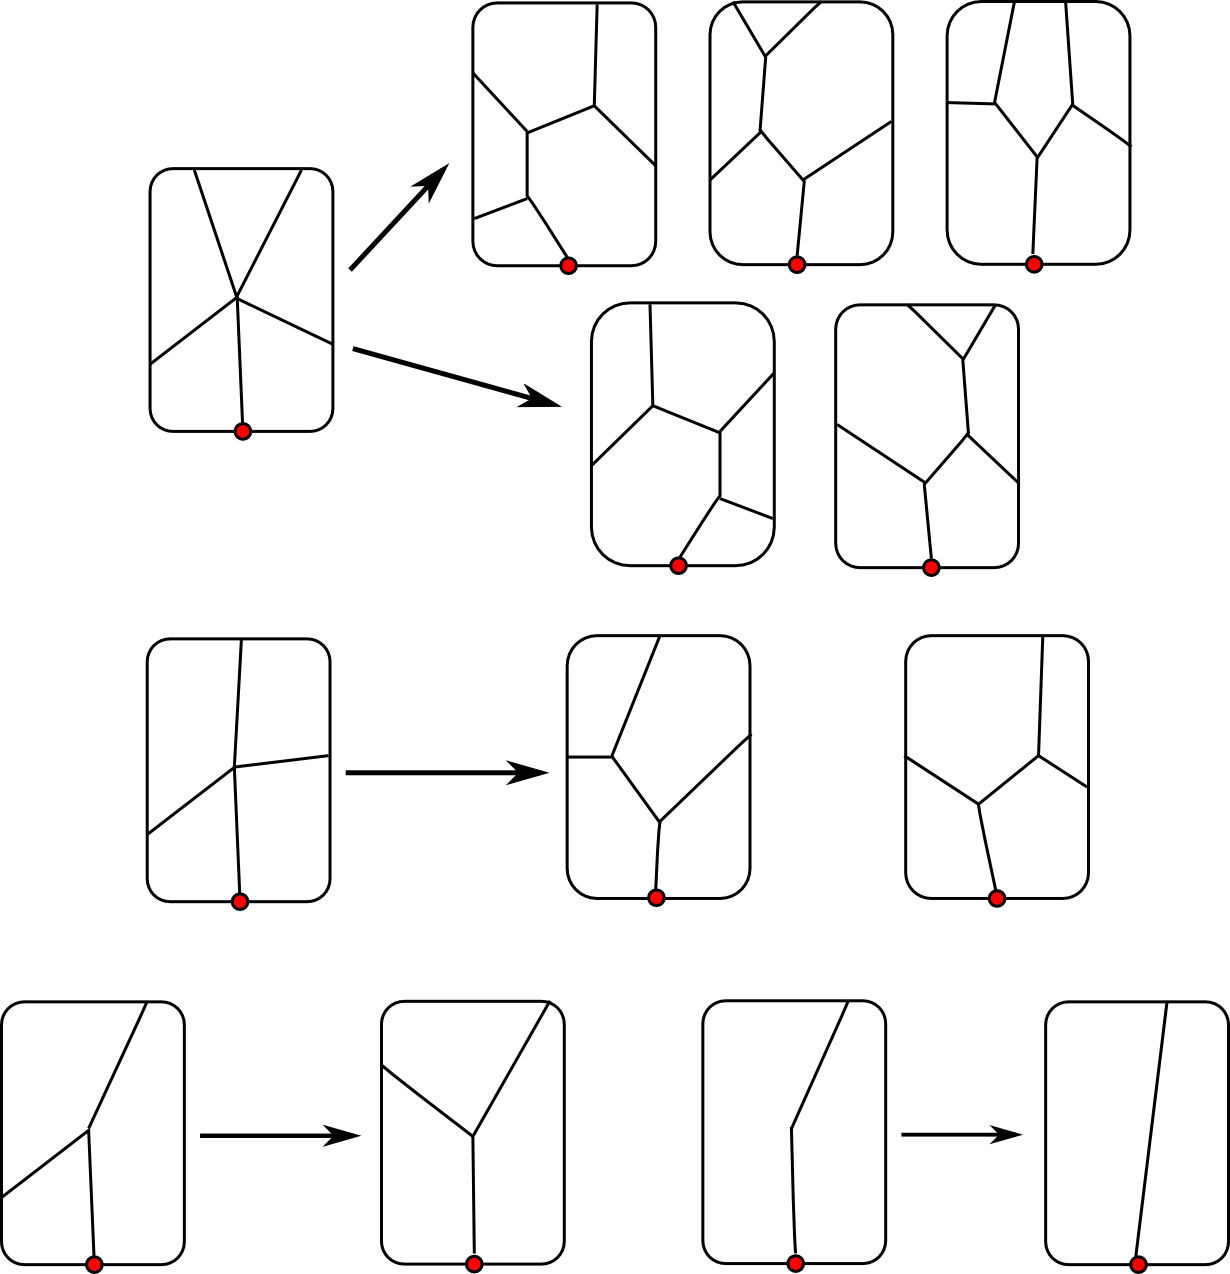
\includegraphics{graintrees.png}
\caption {\textbf{Continuation through a $k$-degree vertex. }\label{crittypes}Possible topologies of  curvature flow with $k$-ray initial conditions, with $k= 3, 4,$ and $5$. These correspond to planar rooted  trivalent tree, with the rooted vertex in each figure denoted by a dot.   } 
\end{centering}   
\end{figure}

We now combine (\ref{vertest}), (\ref{strongfaceest}), and the Euler characteristic formula to obtain
\begin{eqnarray}
V-E+F = 1-k \\
\Rightarrow F =1+\frac{E}3-\frac{2k}3\nonumber\\
\ge1+\frac{7F+3k}{6}-\frac{2k}3 \nonumber\\
\Rightarrow F\le k-6 \nonumber.
\end{eqnarray}
 We therefore search for solutions containing no faces.  Such networks are precisely trees.  Specifically, we seek trivalent trees with $k$ leaves corresponding to  edges containing $p_i$, $i = 1, \dots k$.  Since the endpoints of the leaves are fixed, the number $M_n$ of such trees is equal to the planar trivalent rooted trees of $n$ leaves, which is equal to the ${n-1}^{st}$ Catalan number $C_{n-1}$ \cite{hungerbuhler1995isomorphism}. Specifically, $M_2 = 1,M_3 = 1, M_4 = 2$, and $M_5 = 5$. 
\end{proof}
The explicit graph types are shown in Fig. \ref{crittypes}. However, regardless of topological type, flowing through a  four and five sided grain deletions gives the same topological transitions, as shown in Fig. \ref{distrules}. 


\section{PDMPs and grain coarsening}\label{applygrain}
We now demonstrate that a mean-field model of grain coarsening is a specific example of the $k$-species PDMP explored in \cite{klob2013pdmp1} .  The one parameter constants are as follows, where we index our species $i = 2, \dots, M+1$ according to the $n-gons$ (grains with $n$-sides) they describe:
 
 \begin{centering}
 \begin{tabular}{|c|c|}\hline
General Variable & Value for grain coarsening \\\hline
$M$ & $M>6$ (free parameter)\\\hline
$M_-$ & 4 \\\hline
$\beta$ & $\beta>0$ (free parameter) \\\hline
$v_i$&$i-6 $  \\\hline
$K^{(l)}$&$K^{2}=2, K^{(3)} = 3, K^{(4)}= 2, K^{(5)}= 3, K^{int} = 4$ \\\hline
\end{tabular}

\end{centering}
\vspace{10 pt}
Describing our parameters in more detail:
\begin{itemize}
\item A particle of size $a$ of species $L_n = \mathbb{R}^+, n = 2 ,\dots, M$, corresponds to an $n$-gon with area $a$. 
\item By the $n-6$ rule, the velocity $v_n(a)$ of an $n$-gon is the constant $v_n(a) \equiv n-6$. Thus, $M_- = 4$.
\item Constants $K^{(i)},K^{int}$ correspond to the number of side redistributions for each type of grain  and side deletion, e.g.  five sided grain deletions affect three grains, $K^{(5)} = 3$.     
\end{itemize}

For $n$-gon probability weights, we impose the mean-field assumption that  $n$-gon selection is proportional to $n$.  To obtain a closed system, we forbid two-sided grains to lose sides, three-sided grains to lose two sides, and $M-$sided grains to gain a side. We will not consider one-sided grains, as they are relatively rare in actual metal networks (about .1\%, see \cite{fradkov1985experimental}).  

We now give the explicit weights for $n$-gon selection in grain coarsening.  These are based on the Fradkov assumption that grains are selected based only on their side number. The weights are then
\begin{equation}
w_j^{(2)}= \begin{cases}j, & j \in \{4,\dots, M\},   \ \\
0, & j \in \{2,3\},  \ \\
\end{cases}
\end{equation}
\begin{equation}
w_j^{(3)}= \begin{cases}j, & j \in \{3,\dots, M\},   \ \\
0, & j =2,  \ \\
\end{cases}
\end{equation}
\begin{equation}
w_j^{(4)}= \begin{cases}j, & j \in \{3,\dots, M\},   \ \\
0, & j =2,  \ \\
\end{cases}
\end{equation}
\begin{equation}
w_j^{(5)}= \begin{cases}j, & j \in \{3,\dots, M-1\},   \ \\
0, & j \in\{2,M\},  \ \\
\end{cases}
\end{equation}
\begin{equation}
w_j^{int}= \begin{cases}j, & j \in \{3,\dots, M-1\},   \ \\
0, & j \in\{2,M\}.  \ \\
\end{cases}
\end{equation}

Reassignments are in accordance with  side redistribution under grain and side deletion. Recall the upper index $l= 1, \dots M_-$  in $R_{kj}^{(l)}$ refers to the side number of the deleted grain, $k= 2,\dots, M$ refers to the side number of a neighboring grain before undergoing side reassignment, and $j= 1\dots, K^{(l)}$ refers to the specific reassignment of the $j^th$ grain that is reassigned sides. Refer to Fig. \ref{distrules} for a pictorial description distribution of sides before and after grain and side deletions. Note that we disallow reassignments that create 1 and $M+1$ sided  grains. 
The explicit reassignments are then\begin{equation}
R_{kj}^{(2)}= \begin{cases}k-2, & k \in \{4,\dots, M\},j\in \{1,2\},         \\
0, & k \in \{2,3\} ,  \ \\
\end{cases}
\end{equation}
\begin{equation}
R_{kj}^{(3)}= \begin{cases}k-1, & k \in \{3,\dots ,M\},j\in \{1,2,3\}, \\
0, & k =2,  \ \\
\end{cases}
\end{equation}
\begin{equation}
R_{kj}^{(4)}= \begin{cases}k-1, & k \in \{3,\dots ,M\},j\in \{1,2\}, \\
0, & k =2,  \ \\
\end{cases}
\end{equation}
\begin{equation}
R_{kj}^{(5)}= \begin{cases}k-1, & k\in \{3, \dots,M-1\}, j \in \{1,2\},    \\
k+1, & k\in \{3 ,\dots,M-1\},j=3,\\
0, & k\in \{2 ,M\},\\
\end{cases}
\end{equation}
\begin{equation}
R_{kj}^{int}= \begin{cases}k-1, & k\in \{3, \dots,M-1\}, j \in \{1,2\},    \\
k+1, & k\in \{3 ,\dots,M-1\},j\in\{3,4\},\\
0, & k\in \{2 ,M\}.\\
\end{cases}
\end{equation}

\begin{figure}
\begin{centering}
\includegraphics{grainpic.png}
\caption{\textbf{Reassignments of sides before and after deletions.  }\label{distrules} Numbers in grains refer to side numbers.}
\end{centering}
\end{figure}
We now give an explicit form to the limiting kinetic equations of \cite{klob2013pdmp1} for grain coarsening. Assuming a continuous density of grain areas $u_k(x,t)$, we  can write a system of kinetic equations  for grains with $k$ sides:\begin{equation}\label{grainpde}
\partial_tu_{k}(x,t)+(k-6)\partial_xu_{k}(x,t) = h^{k+}_{grain}(u,t)-h_{grain}^{k-}(u,t)+h^{k+}_{side}(u,t)-h_{side}^{k-}(u,t).
\end{equation}

The four source terms of the right hand side of (\ref{grainpde}) describe, in order, addition and deletion of grains from $L_k$ due to grain deletions, and addition and deletion from $L_k$ due to side deletions.
Explicitly, they are, for $k = 2, \dots, M$,
\begin{eqnarray}
h_{grain}^{k,+}(u,t)= 8u_2(0,t)W_{k+2}^{(2)}(t)u_{k+2}(x,t)+9u_{3}(0,t)W_{k+1}^{(3)}u_{k+1}(x,t)\\+4u_{4}(0,t)W_{k+1}^{(4)}(t)u_{k+1}(x,t)+ 2u_{5}(0,t)W_{k+1}^{(5)}(t)u_{k+1}(x,t)\nonumber\\+u_{5}(0,t)W_{k-1}^{(5)}(t)u_{k-1}(x,t), \nonumber
\end{eqnarray}
\begin{eqnarray}
h_{grain}^{k,-}(u,t) = u_k(x,t)[8u_2(0,t)W_{k}^{(2)}(t)+9u_{3}(0,t)W_{k}^{(3)}(t)\\+4u_{4}(0,t)W_{k}^{(4)}(t)+3u_{5}(0,t)W_{k}^{(5)}(t)],
\nonumber
\end{eqnarray} 
\begin{equation}
h_{side}^{k,-}(u,t)= \frac{2\beta G(t)}{G_{int}(t)}[w_{k-1}^{int}u_{k-1}(x,t)+w_{k+1}^{int}u_{k+1}(x,t)],
\end{equation}
\begin{equation}
h_{side}^{k,+}(u,t)= \frac{4\beta G(t)}{G_{int}(t)}w_k^{int}u_k(x,t),
\end{equation}
for tier weights $w_i^{(l)},w_i^{int}$, total numbers $G(t),G_{int}(t)$, and species selection weight fraction $W_i^{(l)},W_i^{int}$ defined in (\ref{limeq}).
Our main result of the previous chapter is the convergence of empirical PDMPs to the weak form of (\ref{grainpde}) for absolutely continuous measures $\mu_k(t) \in \mathcal{M}(\mathbb{R}^+)$, obtained by pairing solutions $\mu_k$ with a test function $\phi \in \mathcal C$ and integrating along $\mathbb{R}^+$. The weak form of (\ref{grainpde}) is then, for  $k = 2, \dots, M$, 
 \begin{eqnarray}\label{weakgrainpde}
\langle C_k(t), \phi\rangle -  \langle C_k(0), \phi\rangle+(k-6)\int_0^t \langle C_k(s), \phi' \rangle\\= H^{k+}_{grain}(u,t)-H_{grain}^{k-}(u,t)+H^{k+}_{side}(u,t)-H_{side}^{k-}(u,t) ,\nonumber
\end{eqnarray} 
with
\begin{eqnarray}
H^{k+}_{grain}(u,t)=2\int_0^tW^{(2)}_{k+2}(s)\langle C_{k+2}(s), \phi \rangle dF_{2}(s)+\\3\int_0^tW^{(3)}_{k+1}(s)\langle C_{k+1}(s), \phi \rangle dF_{3}(s)+2\int_0^tW^{(4)}_{k+1}(s)\langle C_{k+1}(s), \phi \rangle dF_{4}(s)+ \\2\int_0^\infty W^{(5)}_{k+1}(s)\langle C_{k+1}(s), \phi \rangle+W^{(5)}_{k-1}(s)\langle C_{k-1}(s), \phi \rangle dF_5(s), \nonumber
\end{eqnarray}
\begin{eqnarray}
H_{grain}^{k,-}(u,t) =2 \int_0^t\langle C_{k}(s), \phi \rangle W^{(2)}_{k}(s)dF_2(s)\\+3\int_0^t\langle C_{k}(s), \phi \rangle W^{(3)}_{k}(s)dF_3(s)+2\int_0^t\langle C_{k}(s), \phi \rangle W^{(4)}_{k}(s)dF_4(s)\nonumber\\+3\int_0^t\langle C_{k}(s), \phi \rangle W^{(5)}_{k}(s)dF_{5}(s), \nonumber
\end{eqnarray}
\begin{equation}
H_{side}^{k,-}(u,t)= \int_0^t\frac{2\beta N(s)}{N_o(s)}[w_{k-1}^{int}\langle C_{k-1}(s), \phi \rangle+w_{k+1}^{int}\langle C_{k+1}(s), \phi \rangle]ds,
\end{equation}
\begin{equation}
H_{side}^{k,+}(u,t)= \int_0^t\frac{4\beta N(s)}{N_o(s)}w_{k}^{int}\langle C_{k}(s), \phi \rangle ds.
\end{equation}
A point of departure from the Fradkov model is the choice of side deletion parameter $\beta$.  For the PDMP model, each grain is equipped with a Poisson clock that activates with average time $\beta$.  When such a clock is activated, four grains are selected to change side number in accordance with rules for side flipping.  This differs from Fradkov's model, which assumes side deletion over grain deletion occurs at a constant ratio $\beta$.  Graphs depicting the ratio of side to grain deletions are depicted in Fig. \ref{fradrat1}-\ref{fradrat3}. .  
       


From the previous chapter, we have seen that there exists limiting subsequence that converges to a solution of (\ref{weakgrainpde}).  We now show that the solution retains several properties from the pre-limit PDMP.

\section{Properties of grain coarsening}

One advantage to the stochastic method of proving existence  of solutions to (\ref{weakgrainpde}) is that we can use properties from the finite particle PDMP model to prove, with little difficulty, that the same properties hold for the hydrodynamic limit.  Our main tool is the observation that since $\langle \mu_k^N(t),\phi\rangle \xrightarrow {l.u.} \langle \mu_k(t),\phi\rangle$ for all $\phi \in C_b(\mathbb{R}^+)$, we can choose $\phi \equiv 1$ to obtain the convergence of total numbers $g^N_k(t)\xrightarrow{l.u.} g_k(t)$.

\begin{theorem}  The following properties hold for the limiting distributions $\mu_k(t)$
\begin{enumerate}
\item (\textbf{Conservation of Polyhedral Defect}). If the initial average side number for grains is 6, it remains so:
\begin{equation}
\sum_{k = 2}^M(k-6)g_{k}^0= 0 \quad \Rightarrow \quad P(t):=\sum_{k = 2}^M(k-6)g_k(t)= 0.
\end{equation}
\item (\textbf{No runoff at infinity}).  All loss of total number occurs from boundary events, or
\begin{equation}
N(t) := \sum_{k =2}^M g_k(t) =  \sum_{k = 2}^M g_{k}^0-\sum_{i = 2}^5 F_i(t).
\end{equation}
\item (\textbf{Decreasing densities}).  The total number is decreasing in time:
\begin{equation}
N(t)\le N(s) \quad \hbox{ for } t\ge s.
\end{equation}
\end{enumerate}
\end{theorem}
\begin{proof}
Suppose we have a limiting initial measure $\mu_k^0$ with zero polyhedral defect. For $i \in \mathbb N$, let $\mu_k^{N_i,0}\in \mathcal M(\mathbb R^+)$  be a sequence of initial empirical distributions of particles with zero polyhedral defect, satisfying $\mu_k^{N_i,0} \rightarrow \mu_k^0 $ in $\mathcal M(\mathbb{R}^+)$. Constructing such a sequence is always possible. To see this, choose integers $N_i \rightarrow \infty$  ,where $N_i= N_i^2+\dots+N_i^M$ , $\sum_{k = 2}^M (k-6)N_i^k = 0 $, and $N_i^k/\sum_j N_i^j \rightarrow g_{i,0}$. For each $n$-gon in $L_n$, randomly select $N_i^k$ particles with respect to the distribution $\mu_k^0$.  By the Glivenko-Cantelli theorem, with probability one the empirical distributions  $\mu_k^{N_i,0}$ will converge  to $\mu_k^0$ in $\mathcal M(\mathbb{R}^+)$.  
 
For the empirical measures $\mu^{N_i,0}(t)$, it is straightforward to see conservation of polyhedral defect.  This is because transport of grains does not change a grain's side number, and one can check that any critical event has a net zero change in polyhedral defect. Thus  
\begin{equation}
P^{N_i}(t) :=\sum_{k = 2}^M(k-6)g_k^{N_i}(t)= 0.     
\end{equation}
Since $g_k$ is the local uniform limit of $g_k^{N_i}(t)$, we obtain property (1).

For property (2), we again choose a sequence of empirical initial measures $\mu_k^{N_,0} \rightarrow \mu_k^0 $ in $\mathcal M(\mathbb{R}^+)$, this time with no further qualifications. For the empirical densities, we have 
\begin{equation}\label{totalmass}
\sum_{k =2}^M g_k^N(t) =  \sum_{k = 2}^M g_{k,0}^{N}-\sum_{i = 2}^5 F_i^N(t). \end{equation}
In the previous chapter we've shown that $F_i^N(t) \xrightarrow{l.u.} F_i(t)$, so taking the local uniform limit proves (2).  Statement (3) then follows immediately from (\ref{totalmass}), as the cumulative distributions $F_i$ are increasing.     
\end{proof}


Our next task is to show that our system conserves area, which is a consequence of conservation of polyhedral defect.  In this case, we'll  use the weak form of the limiting equations.  Here, we denote the identity function $id: x \mapsto x$.     
\begin{theorem}(\textbf{Conservation of area}).  For initial distributions which satisfy
\begin{equation}
\sum_{k = 2}^M\langle \mu_k^0,id\rangle< \infty, \quad P(0) = 0, 
\end{equation} 
we have 
\begin{equation}
\sum_{k = 2}^M\langle \mu_k(t),id\rangle = \sum_{k = 2}^M\langle \mu_k^0,id\rangle
\end{equation}
\end{theorem}
\begin{proof}  For $r,j>0$, we use functions $\phi^{r,j}:\mathbb{R}^+ \rightarrow \mathbb{R}^+$ defined by
\begin{equation}
\phi^{r,j}(x) = \begin{cases}x & x<r \\
\psi^{j}(x-r)+r & x \in [r,r+\frac 1j] \\
r  \ & x > r+\frac 1j,
\end{cases}
\end{equation}
where $\psi^j:[0,\frac 1j]\rightarrow \mathbb{R}^+$ is a $C^1(\mathbb{R}^+)$ function with $\psi'(0) = 1$ and $\psi'(\frac1j) = 0$, so that $\phi^{r,j}\in \mathcal C$.  If we sum (\ref{grainpde})  over grain classes, a simple  (though lengthy) calculation shows that
\begin{equation}
\sum_{k = 2}^MH^{k+}_{grain}(u,t)-H_{grain}^{k-}(u,t)+H^{k+}_{side}(u,t)-H_{side}^{k-}(u,t)= 0.
\end{equation}
Intuitively, this identity simply states that critical events change side numbers of grains, but not their areas.  We are left with the relation
\begin{equation}\label{finitearea}
\sum_{k = 2}^M\langle \mu_k(t), \phi^{r,j}\rangle =  \sum_{k = 2}^M\langle \mu_k(0), \phi^{r,j}\rangle-\sum_{k = 2}^M(k-6)\int_0^t \langle \mu_k(s), (\phi^{r,j})' \rangle.
\end{equation}
Notice, however, that 
\begin{equation}
\langle \mu_k(s), (\phi^{r,j})' \rangle= \mu_k(s)([0,r))+\int_0^{\frac 1j}\psi^j d\mu_k(s) \rightarrow g_k(s) \hbox{ as } r,j\rightarrow \infty.
\end{equation}  
This implies that taking the limit as $j,r\rightarrow \infty$ in (\ref{finitearea}) gives
\begin{equation}
 \sum_{k = 2}^M\langle \mu_k(t), id\rangle =  \sum_{k = 2}^M\langle \mu_k(0), id\rangle-\int_0^t P(s)ds.
\end{equation}
Our theorem then follows from conservation of polyhedral defect.
\end{proof}

\section{Computations}\label{computations}
Simulations for PDMP grain coarsening were performed in Matlab. Grains over several different initial configurations and $\beta$ parameters were tested. Illustrations, unless otherwise noted, are with $N= 9\times 10^4$ initial grains with a maximum of 20 sides. \textbf{Uniform initial distributions} have $10^4$ $n$-gons, for $n=2, \dots, 10$, distributed uniformly in $[0,1]$.   At time  $t= 5$ the number of grains drops an order of magnitude (see figure \ref{grainnumber}).  We observe the following:
\subsection*{Mean area growth}
Simulations of grain networks which directly approximate mean curvature flow suggest that the average grain area grows linearly.   (see, \cite{elsey2009diffusion,anderson1984computer,wakai2000three}, for instance). In our simulations, the plot the average area $\langle A_\beta(t)\rangle$ at time $t$ for the grain coarsening PDMP with varying Poisson parameters $\beta$. For small values of $\beta$,   $\langle A_\beta(t)\rangle$ is approximately linear (see Fig. \ref{av1},\ref{av2}).  The same behavior holds for average area of grains with $k$ sides, $k = 1, \dots, M$. For larger values of $\beta$, coarsening becomes convex (Fig. \ref{av3}).

\subsection*{Distribution of $n$-gons} For low values of $\beta$, the distribution of $n$-gons is approximately stationary (see Fig. \ref{sidedist1}) .  However, as $\beta$ increases, distributions of  $n$-gons $n= 3, \dots, 9$ become more uniform  as time increases (Fig. \ref{sidedist3}). This is similar to the numerical experiments of Fradkov \cite{fra881}.   Plots of $n$-gon densities for $\beta = 0$ and the Kinderlehrer model described in \cite{kin06} for stationary densities (time $t= 5$ for both models) shows a similarity of  statistics (see Fig. \ref{kindcompare}).    

 \subsection*{Grain densities and diffusion} In Fig. \ref{tierdens1}-\ref{tierdens9}, we plot histograms for grain densities of 4, 6, and 8 sides under $\beta$ values of .01, .1, and 1.  Each bar represent a bin of 40 grains. From grain deletions, the number of bars decreases, corresponding to a decrease in number for increasing time.  The densities for all $n$-gons drift to the right with time (see Fig. \ref{averagewhole}).  The parameter $\beta$ appears to play a diffusing role, as larger $\beta$ also correspond to increased variance.  
   
\subsection*{Side to grain deletion ratio} As observed in Section \ref{applygrain}, the PDMP model differs from the Fradkov model in its choice of parameter $\beta$. Thus, we will denote $\gamma_{\beta}(t)$ as the (time dependent) ratio of side deletions to grain deletions. For a uniform initial distribution,  under differing $\beta$,  $\gamma_{\beta}(t)$ exhibits similar concave profiles   (see Fig. \ref{fradrat1}-\ref{fradrat3}).









\section{Remarks}


A major advantage to viewing grain growth statistics as approximations of a hydrodynamic limit  is the relative ease of implementing simulations.  As we have seen, we can immediately raise several conjectures about grain behavior.  For example, for $\beta = 0$, does there exist a stable attractor for the distribution of $n$-gon densities?  Several details of the limiting densities make this question difficult.  First, individual $n$-gon densities do not have stable attractors.  Also, we still have yet to establish existence for an infinite time, which would be central in an asymptotic analysis.  Such long time existence was established for the Fradkov system in \cite{henseler2008kinetic}, but the existence of universal attractors in this model remains unanswered.        

   The role of the flipping parameter $\beta$ plays an interesting role in altering grain statistics. The general trend noted in simulations is that $\beta$ tends to act as a diffusion agent between $n$-gons. The rule for side flipping is similar to the particle transfer rule in the following model, as described in \cite{bruus2008theoretical}.  Here, we are approximating the dispersal of a fluid plug with initial density $u_{0}(x,y)$ in a carrier fluid. If the fluid has a vertical velocity profile of $V(y)$, the governing equations for the evolving density $u(x,y,t)$ have the form
\begin{eqnarray}
u_t-V(y)u_{x} = \frac{\alpha}2 u_{yy}\\
u(x,y,0) = u_0(x,y). \nonumber
\end{eqnarray}
The factor $\alpha$ is the diffusivity factor for the plug.  Taken as a $k$-species PDMP, we can approximate the domain carrier fluid by a large number of horizontal tiers, and then approximately the fluid plug as particles traveling on these tiers with velocity $V(y^*)$ for a tier located at $y = y^*$.  This model has no particle deletions (the fluid is conserved), but each particle is equipped with a Poisson clock of parameter $\alpha$, that when set, transfers a particle  to the next highest species with probability 1/2, and to the next lowest species with probability 1/2.  This, rule, however, is roughly the same as side flipping. In both models, for $n$ particles that are selected in an intermediate species, roughly $n/2$ will transfer upwards by one species, and $n/2$ will lower by a species. Thus, it is reasonable to expect the $\beta$ parameter in grain coarsening to act in a similar manner as the diffusion parameter $\alpha$ for the fluid plug. This is, of course, not precise, as we have not actually shown the right scaling of vertical species interspacing for the fluid plug, nor have we considered how grain deletions may interact with  diffusion due to side deletion.
\begin{figure}
\hspace{130pt}\includegraphics[width=.3\textwidth]{fluidpic.png} 
\caption{\textbf{Dispersal of a fluid plug.}  A carrier fluid   is approximated by horizontal tiers, and a fluid plug (the inner region of the figure) is approximated by particles (denoted by dots) which travel horizontally on tiers corresponding to the vertical velocity profile $V(y)$.}
\end{figure}

 
\clearpage{}

\begin{figure}
   \begin{centering}     
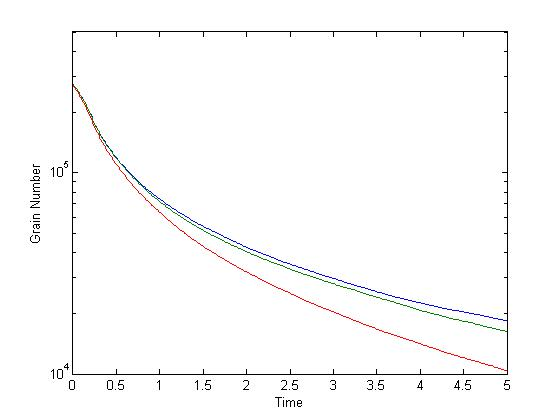
\includegraphics[width=.5\textwidth]{grainnumber.jpg}
        \caption{\textbf{Grain number} $N(t)$.}\label{grainnumber}
        \end{centering}
  \end{figure}

 \begin{figure}
 \begin{centering}
  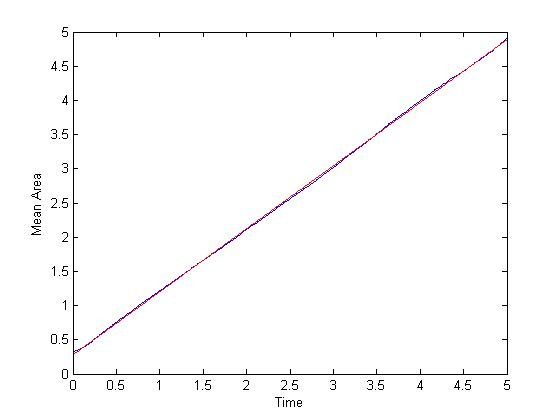
\includegraphics[width=.5\textwidth]{meanregareazero.jpg}
\caption{\textbf{Mean area of grains with $\beta = .01$} Mean area is plotted with line of best fit $y_1 = .2806+.9214x$  (the lines are indistinguishable). The correlation between average area and $y_1$ is $r^2= .9998$. }\label{av1}
\end{centering}
\end{figure}

\begin{figure}
  \begin{centering}
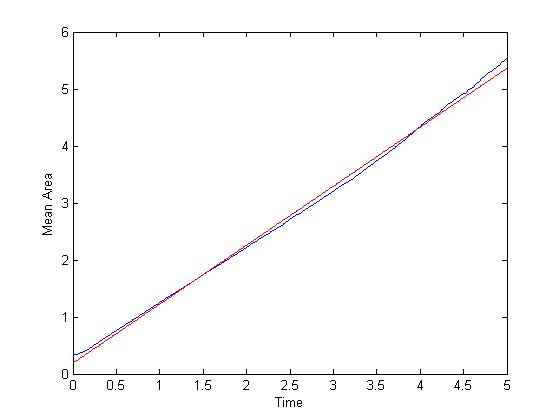
\includegraphics[width=.5\textwidth]{meanregareatenth.jpg}
\caption{\textbf{Mean area of grains with $\beta = .1$} Mean area is plotted with line of best fit $y_1 = .1909+1.0347x$   (the lines are almost indistinguishable). The correlation between average area and $y_1$ is $r^2= .9979$. }\label{av2}
\end{centering}
\end{figure}

\begin{figure}
  \begin{centering}
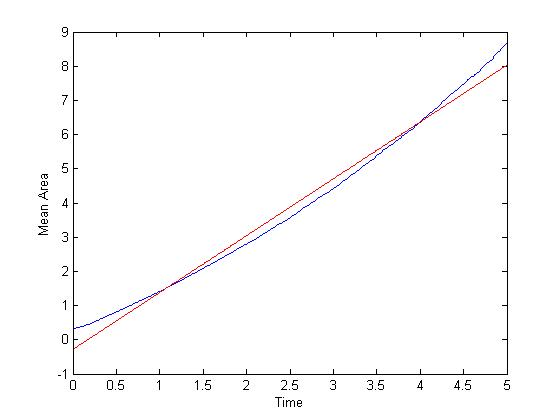
\includegraphics[width=.5\textwidth]{meanregareaone.jpg}
\caption{\textbf{Mean area of grains with $\beta = 1.$} Mean area is plotted with line of best fit $y_1 = -.2796+1.6624x$   (mean area is convex). The correlation between average area and $y_1$ is $r^2= .9881$. }\label{av3}
\end{centering}
\end{figure}



\begin{figure}
\begin{centering}
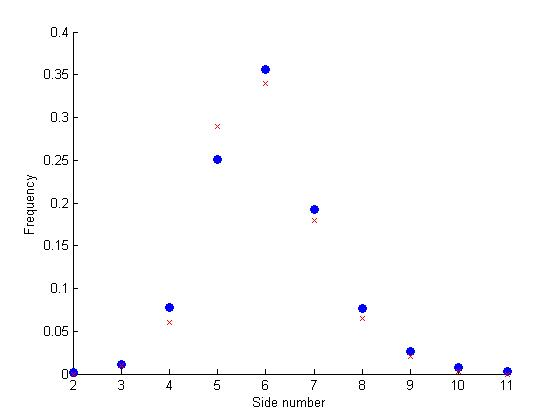
\includegraphics[width=.5\textwidth]{kindocompare.jpg}
\caption{Comparison of side number frequency between grain coarsening PDMP (dots) at $\beta= 1$ and the Kinderlehrer model (crosses) at $t= 5$.}\label{kindcompare}
\end{centering}
\end{figure}

\begin{figure}
        \begin{centering}
        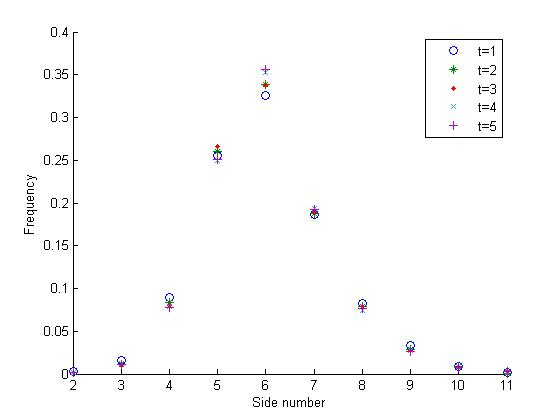
\includegraphics[width=.5\textwidth]{classdistzero.jpg}
        \caption{Frequency of side number for $\beta= .01$ for various times.}\label{sidedist1}
\end{centering}
\end{figure}

\begin{figure}
        \begin{centering}
        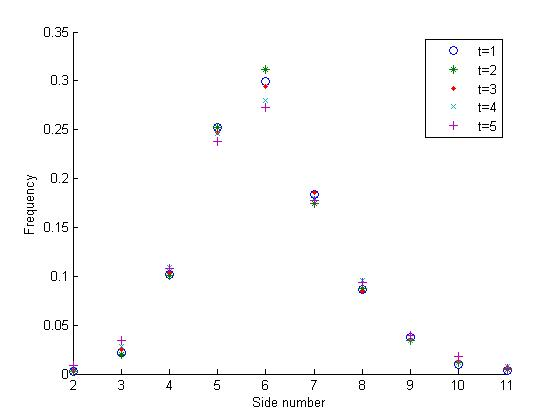
\includegraphics[width=.5\textwidth]{classdisttenth.jpg}
        \caption{Frequency of side number for $\beta= .1$ for various times.}
\end{centering}
\end{figure}

\begin{figure}
        \begin{centering}
        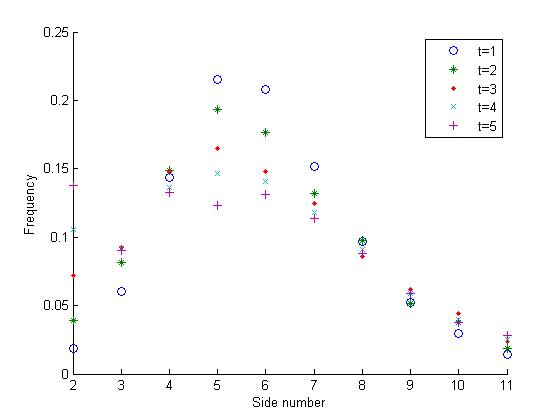
\includegraphics[width=.5\textwidth]{classdistone.jpg}
        \caption{Frequency of side number for $\beta= 1$ for various times.}\label{sidedist3}
\end{centering}
\end{figure}
        
        
        
        

 




       
        
        
        





        
        
       


\begin{figure}
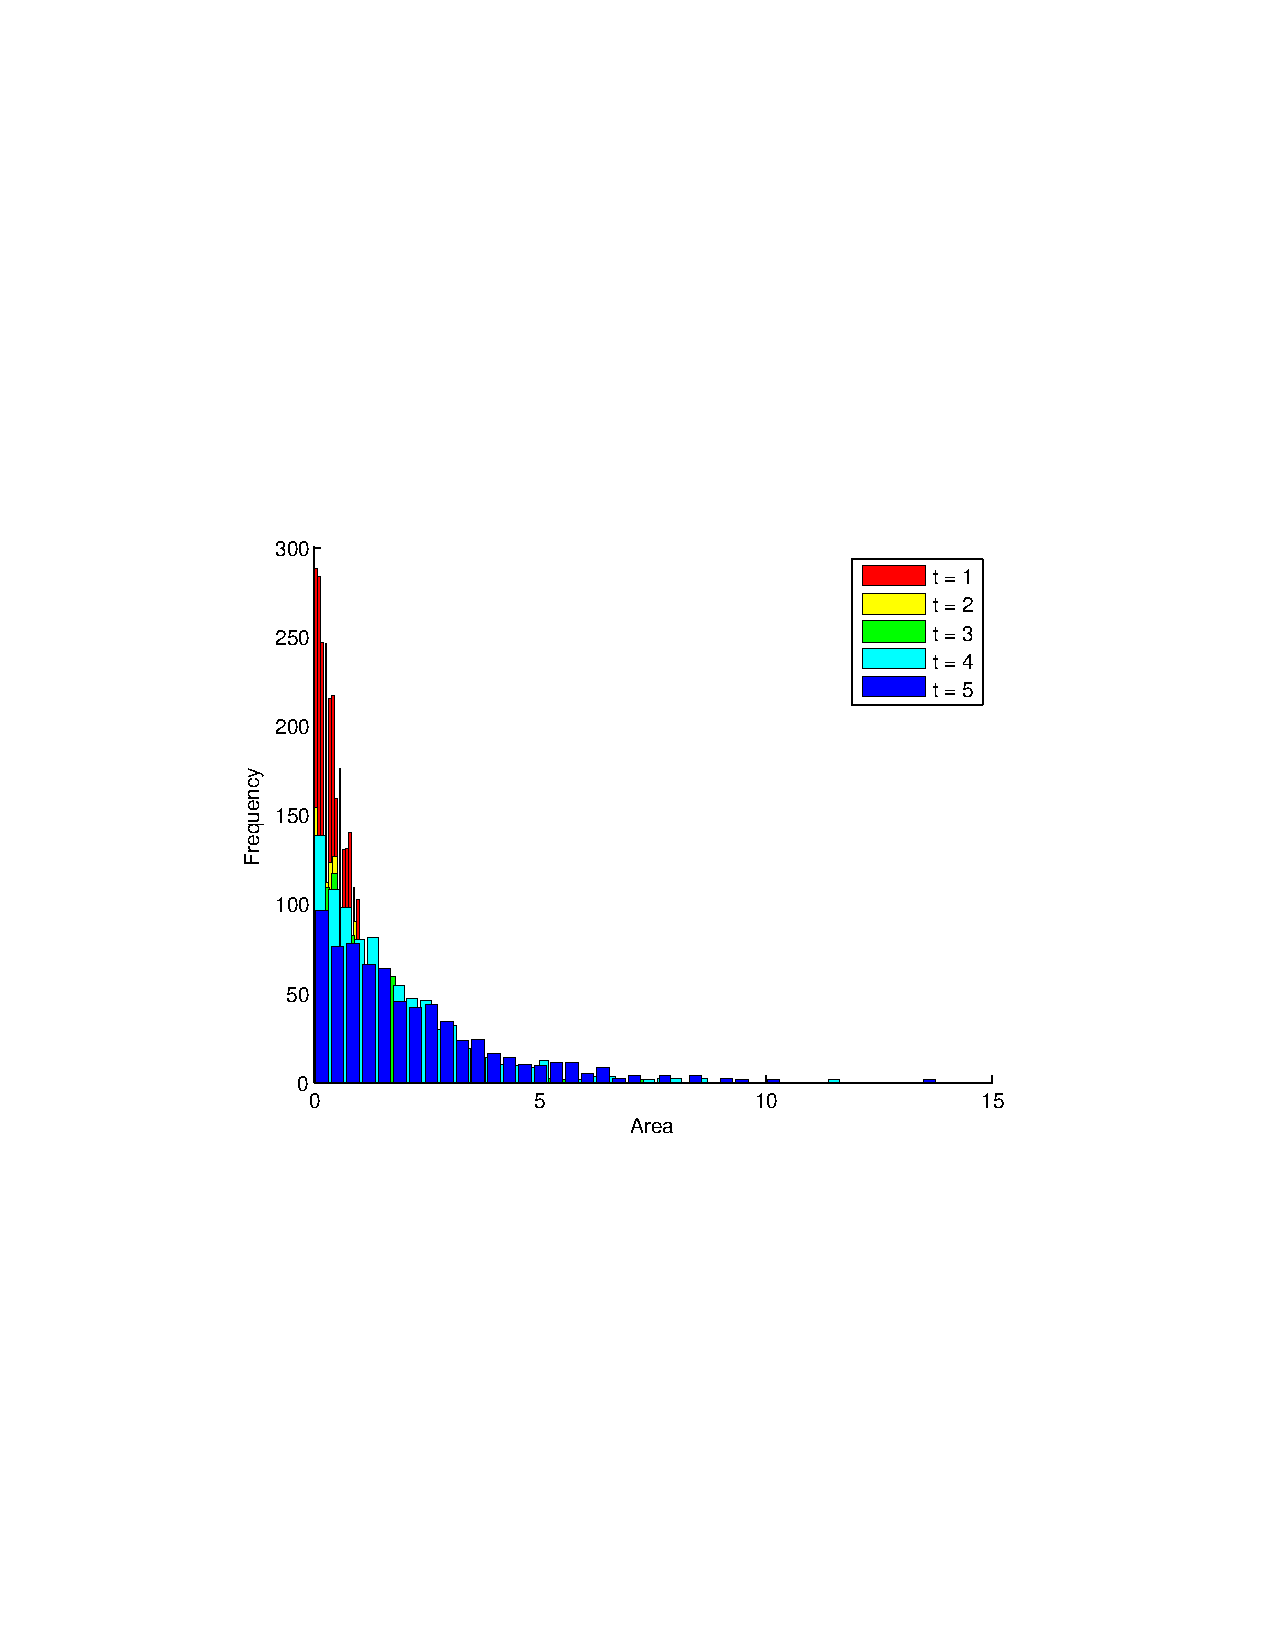
\includegraphics[width=\textwidth]{histbetazerotier4.pdf}
\vspace{-130pt}
\caption{Histograms of four-sided grain densities at $\beta = .01$.}\label{tierdens1}
\end{figure}

\begin{figure}
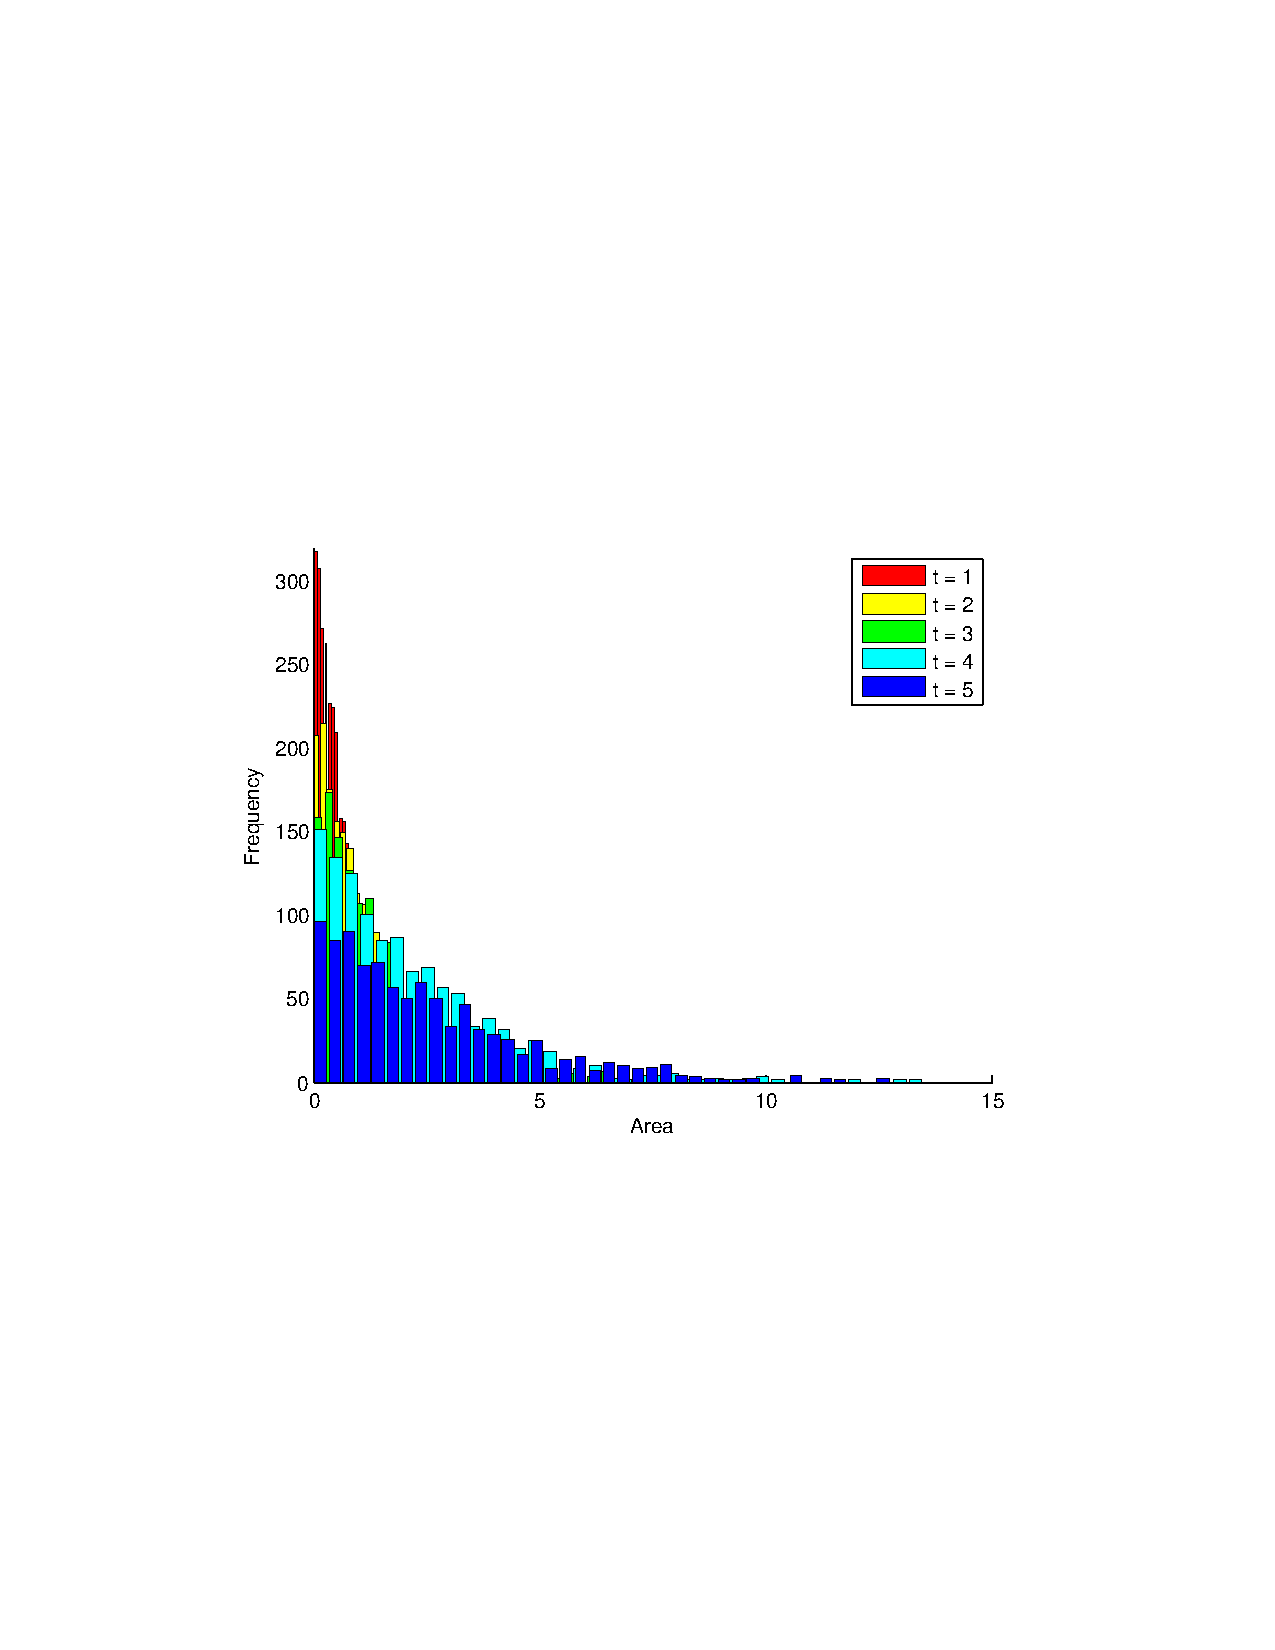
\includegraphics[width=\textwidth]{histbetatenthtier4.pdf}
\vspace{-130pt}
\caption{Histograms of four-sided grain densities at $\beta = .1$.}
\end{figure}

\begin{figure}
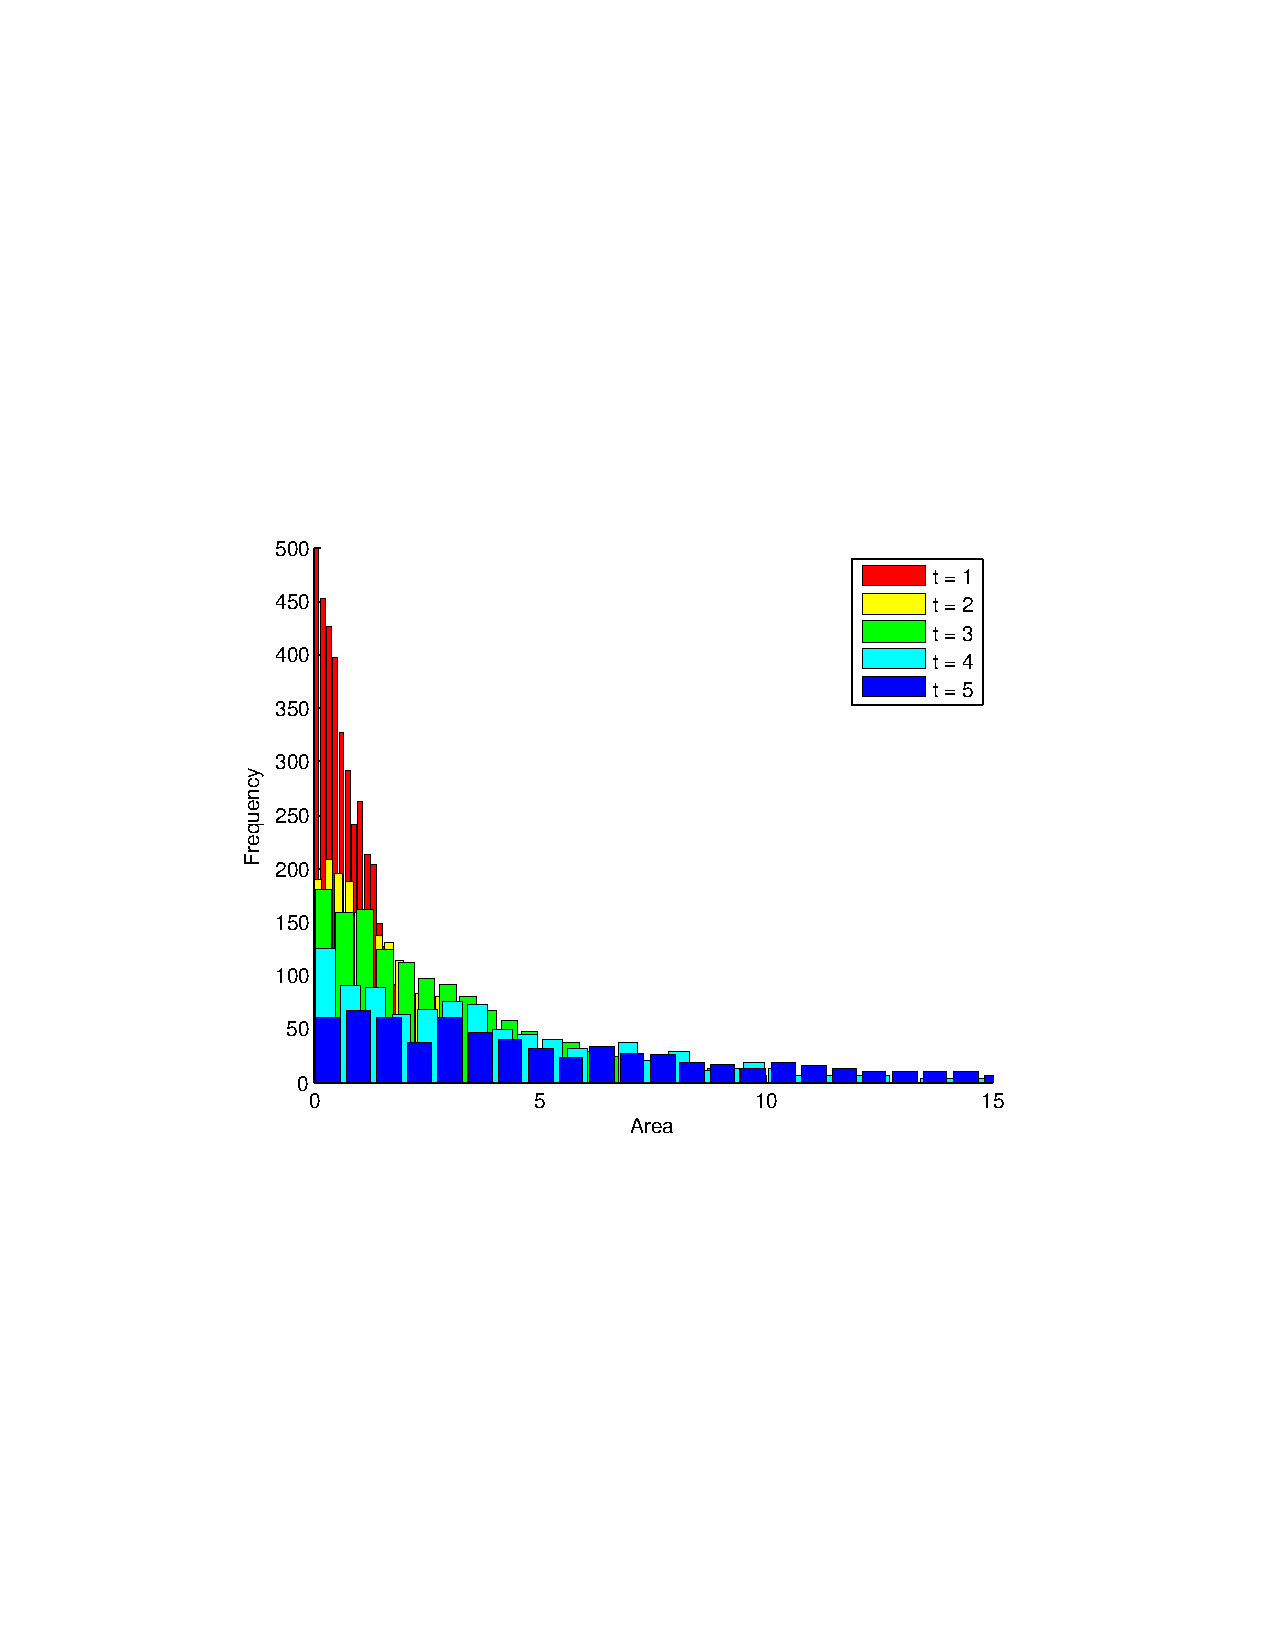
\includegraphics[width=\textwidth]{histbetaonetier4.pdf}
\vspace{-130pt}
\caption{Histograms of four-sided grain densities at $\beta = 1$.}
\end{figure}

\begin{figure}
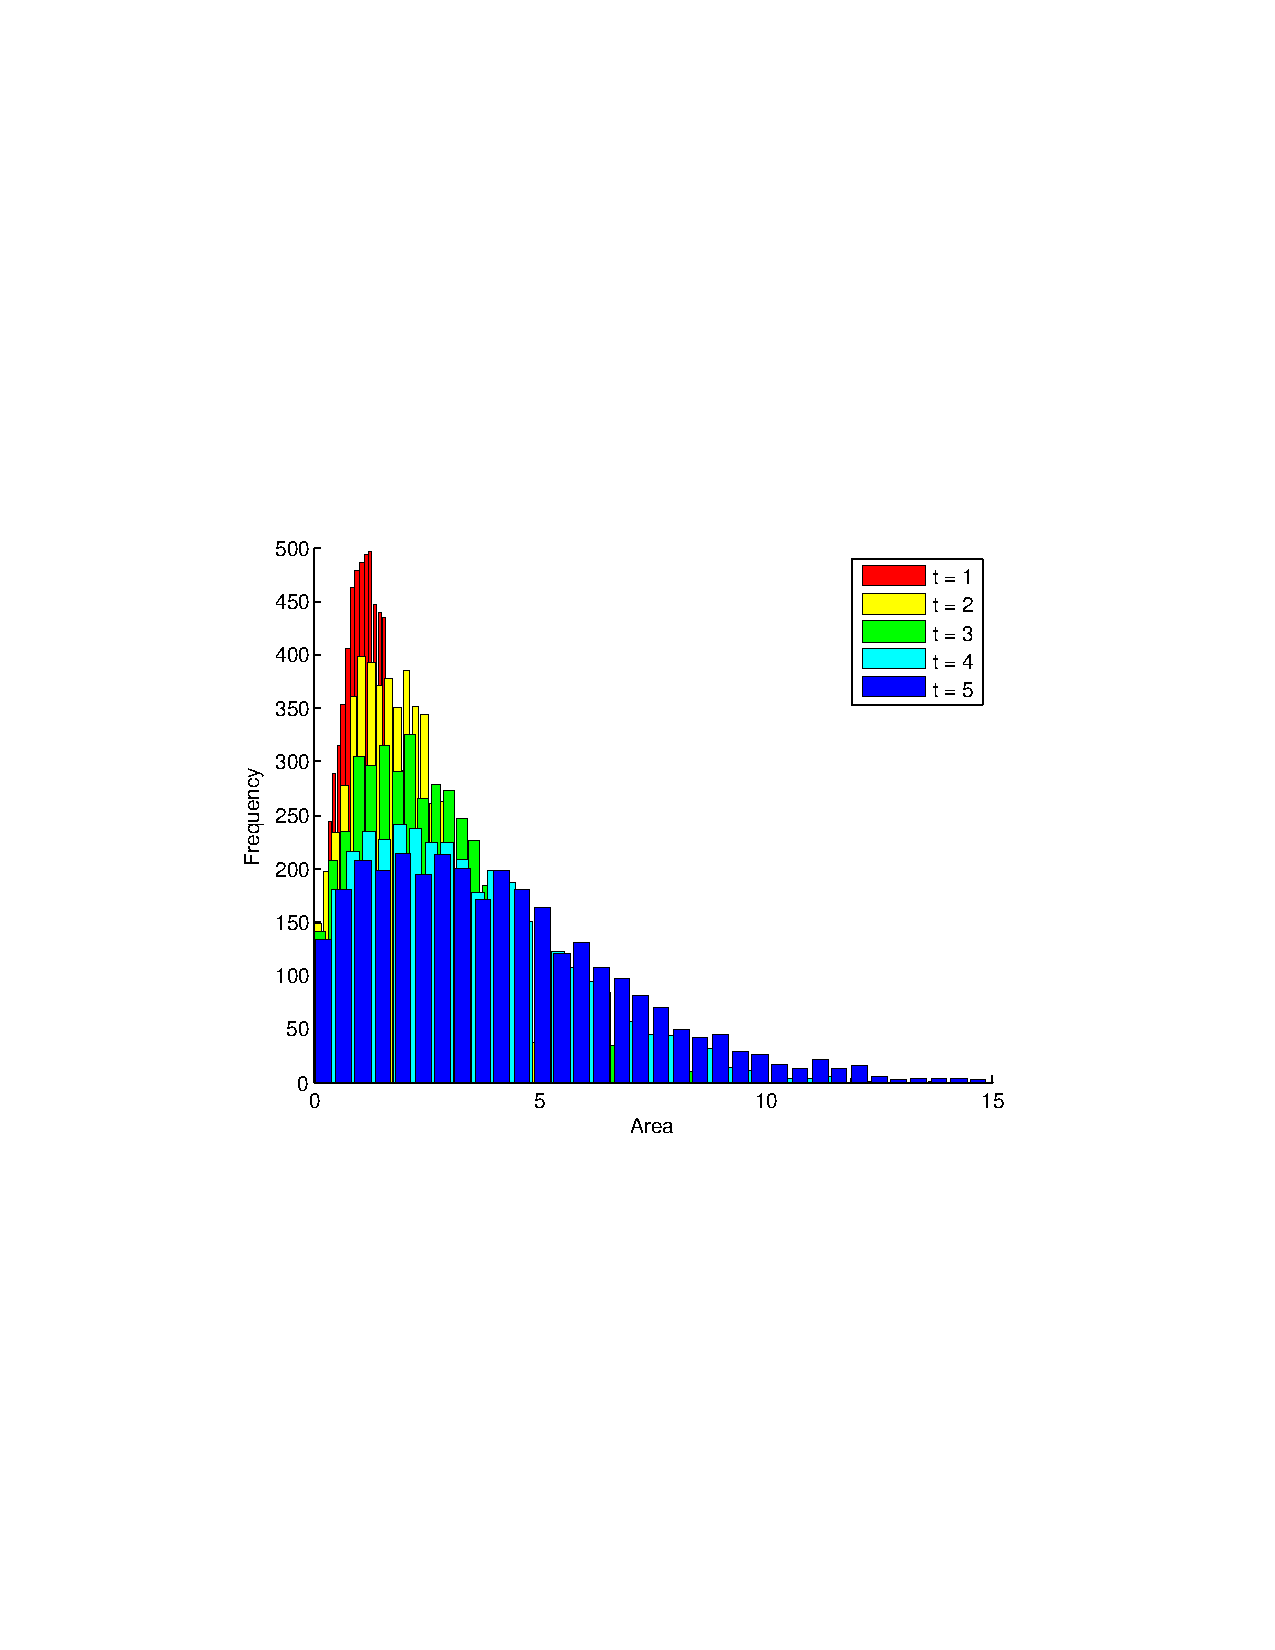
\includegraphics[width=\textwidth]{histbetazerotier6.pdf}
\vspace{-130pt}
\caption{Histograms of six-sided grain densities at $\beta = .01.$}
\end{figure}

\begin{figure}
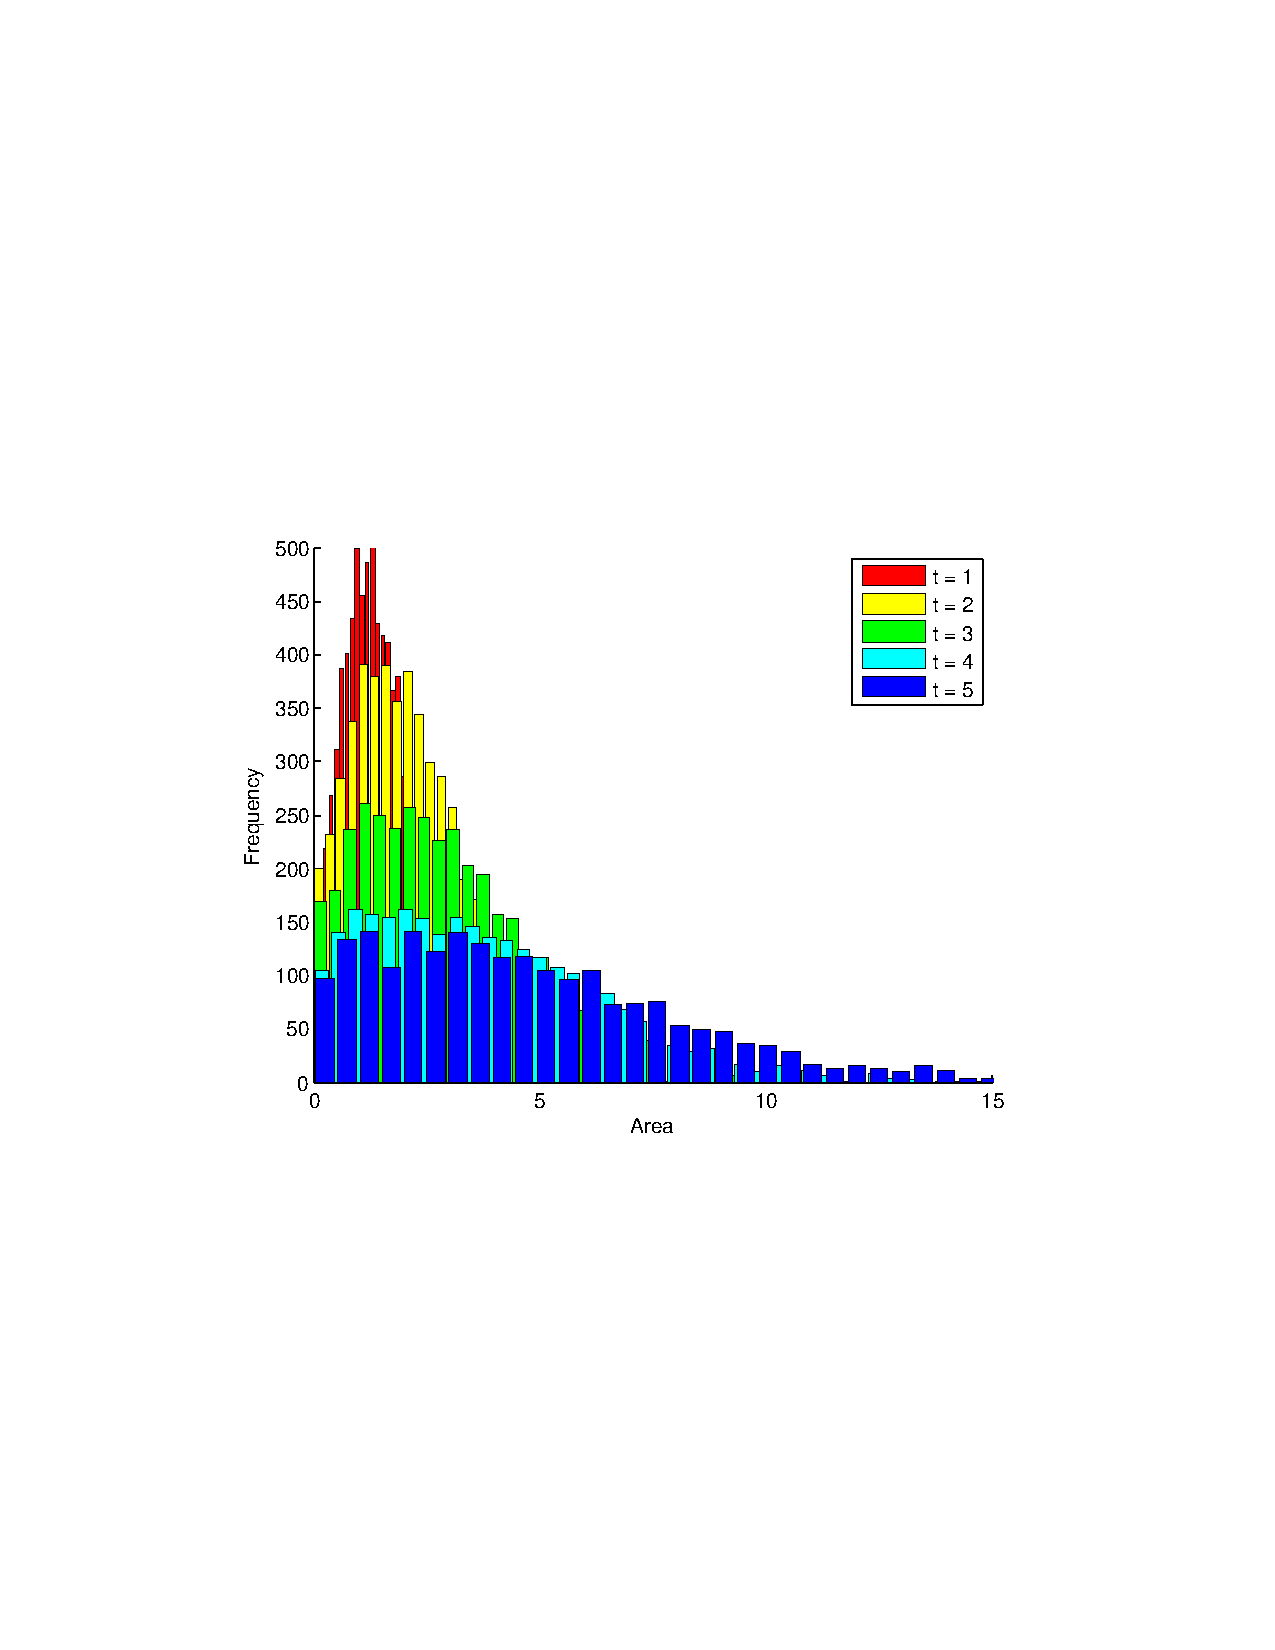
\includegraphics[width=\textwidth]{histbetatenthtier6.pdf}
\vspace{-130pt}
\caption{Histograms of six-sided grain densities at $\beta = .1$.}
\end{figure}

\begin{figure}
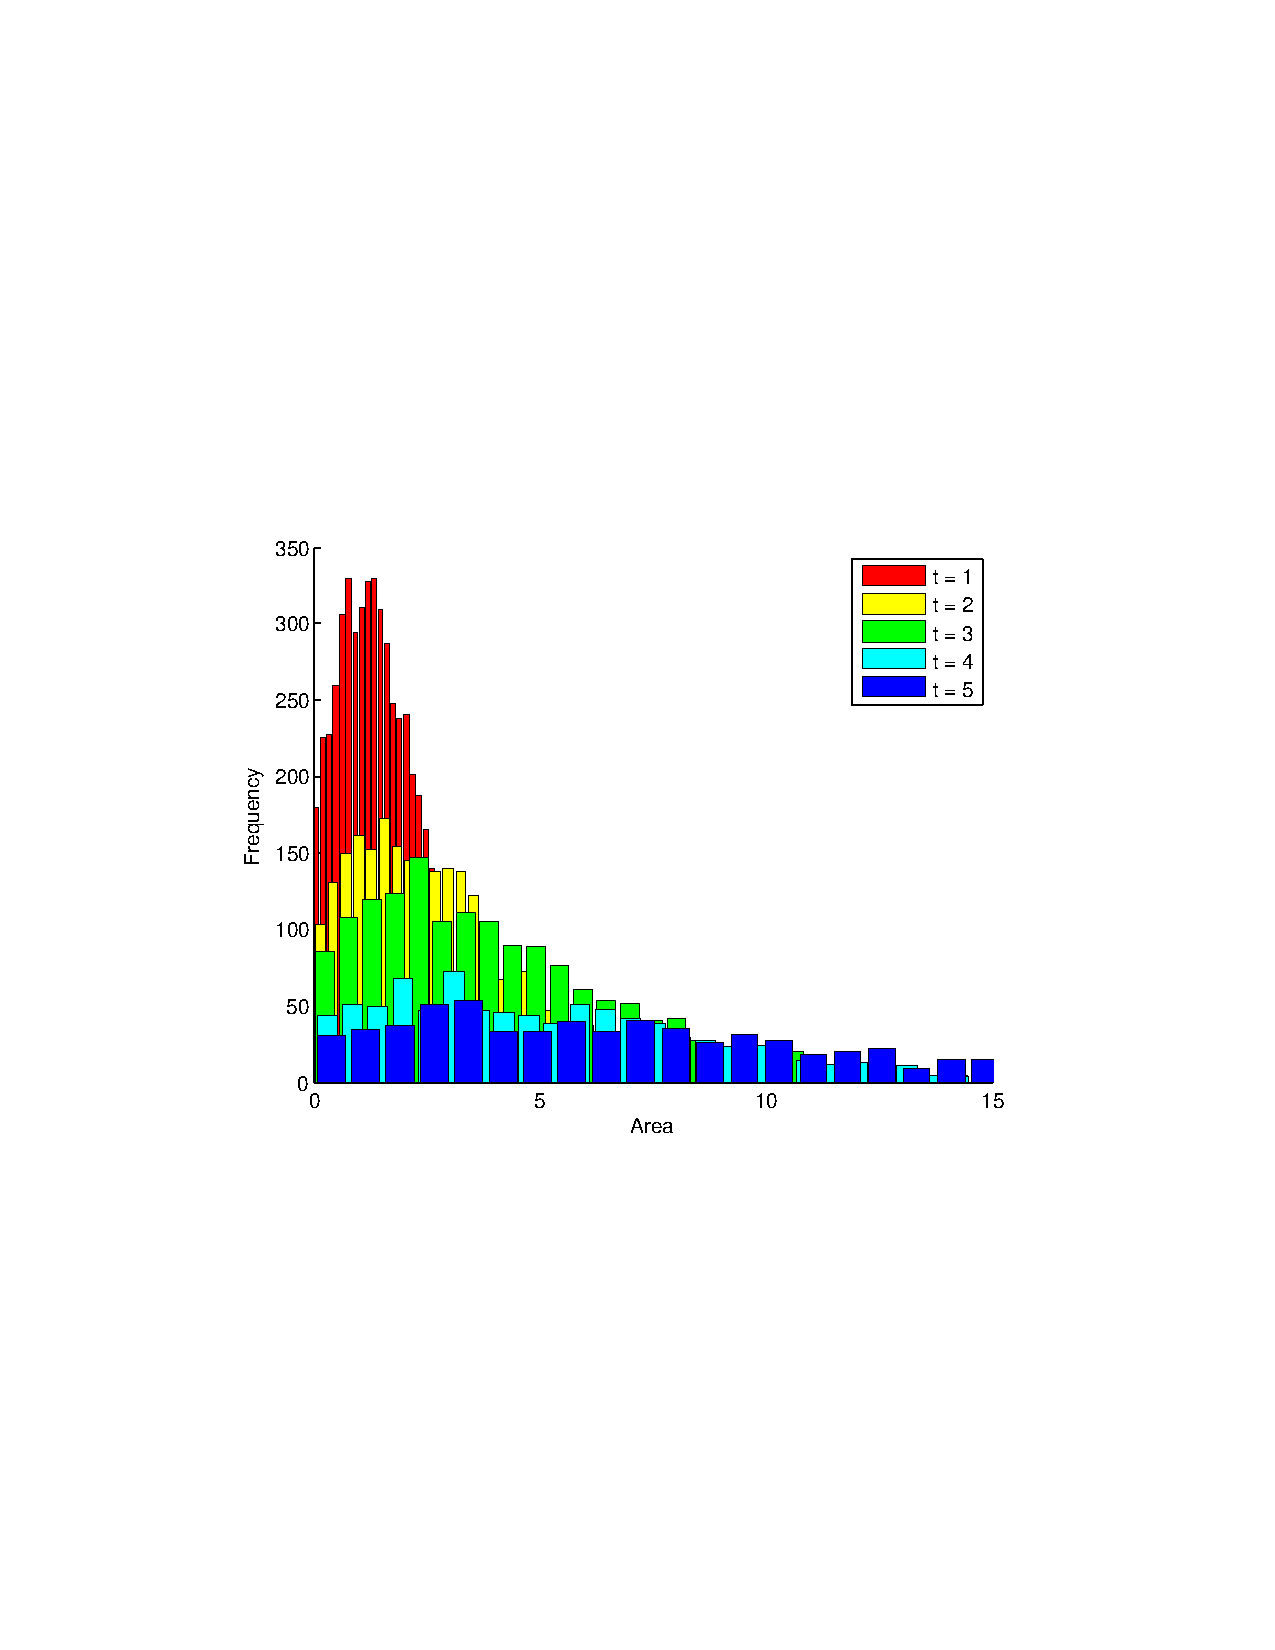
\includegraphics[width=\textwidth]{histbetaonetier6.pdf}
\vspace{-130pt}
\caption{Histograms of six-sided grain densities at $\beta = 1$.}
\end{figure}

\clearpage{}


\begin{figure}
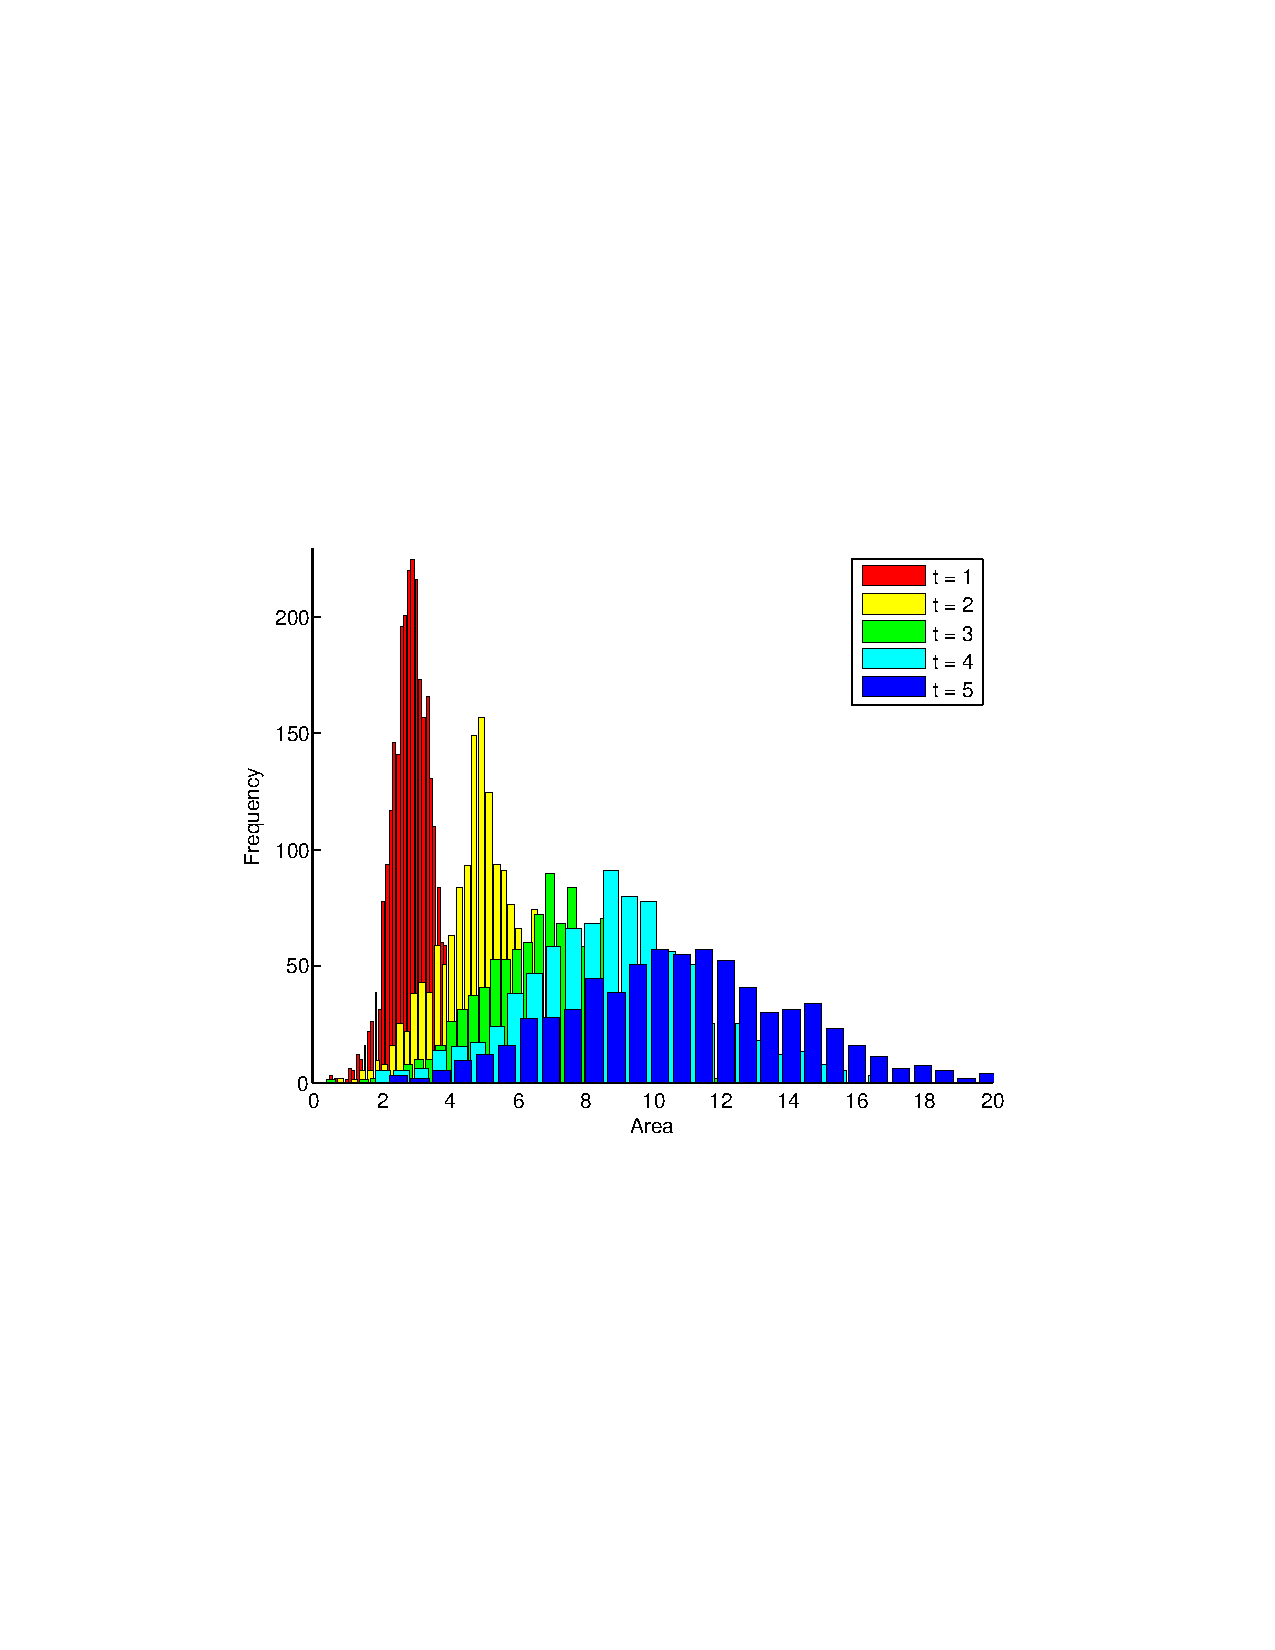
\includegraphics[width=\textwidth]{histbetazerotier8.pdf}
\vspace{-130pt}
\caption{Histograms of eight-sided grain densities at $\beta = .01$.}
\end{figure}

\clearpage{}
\begin{figure}
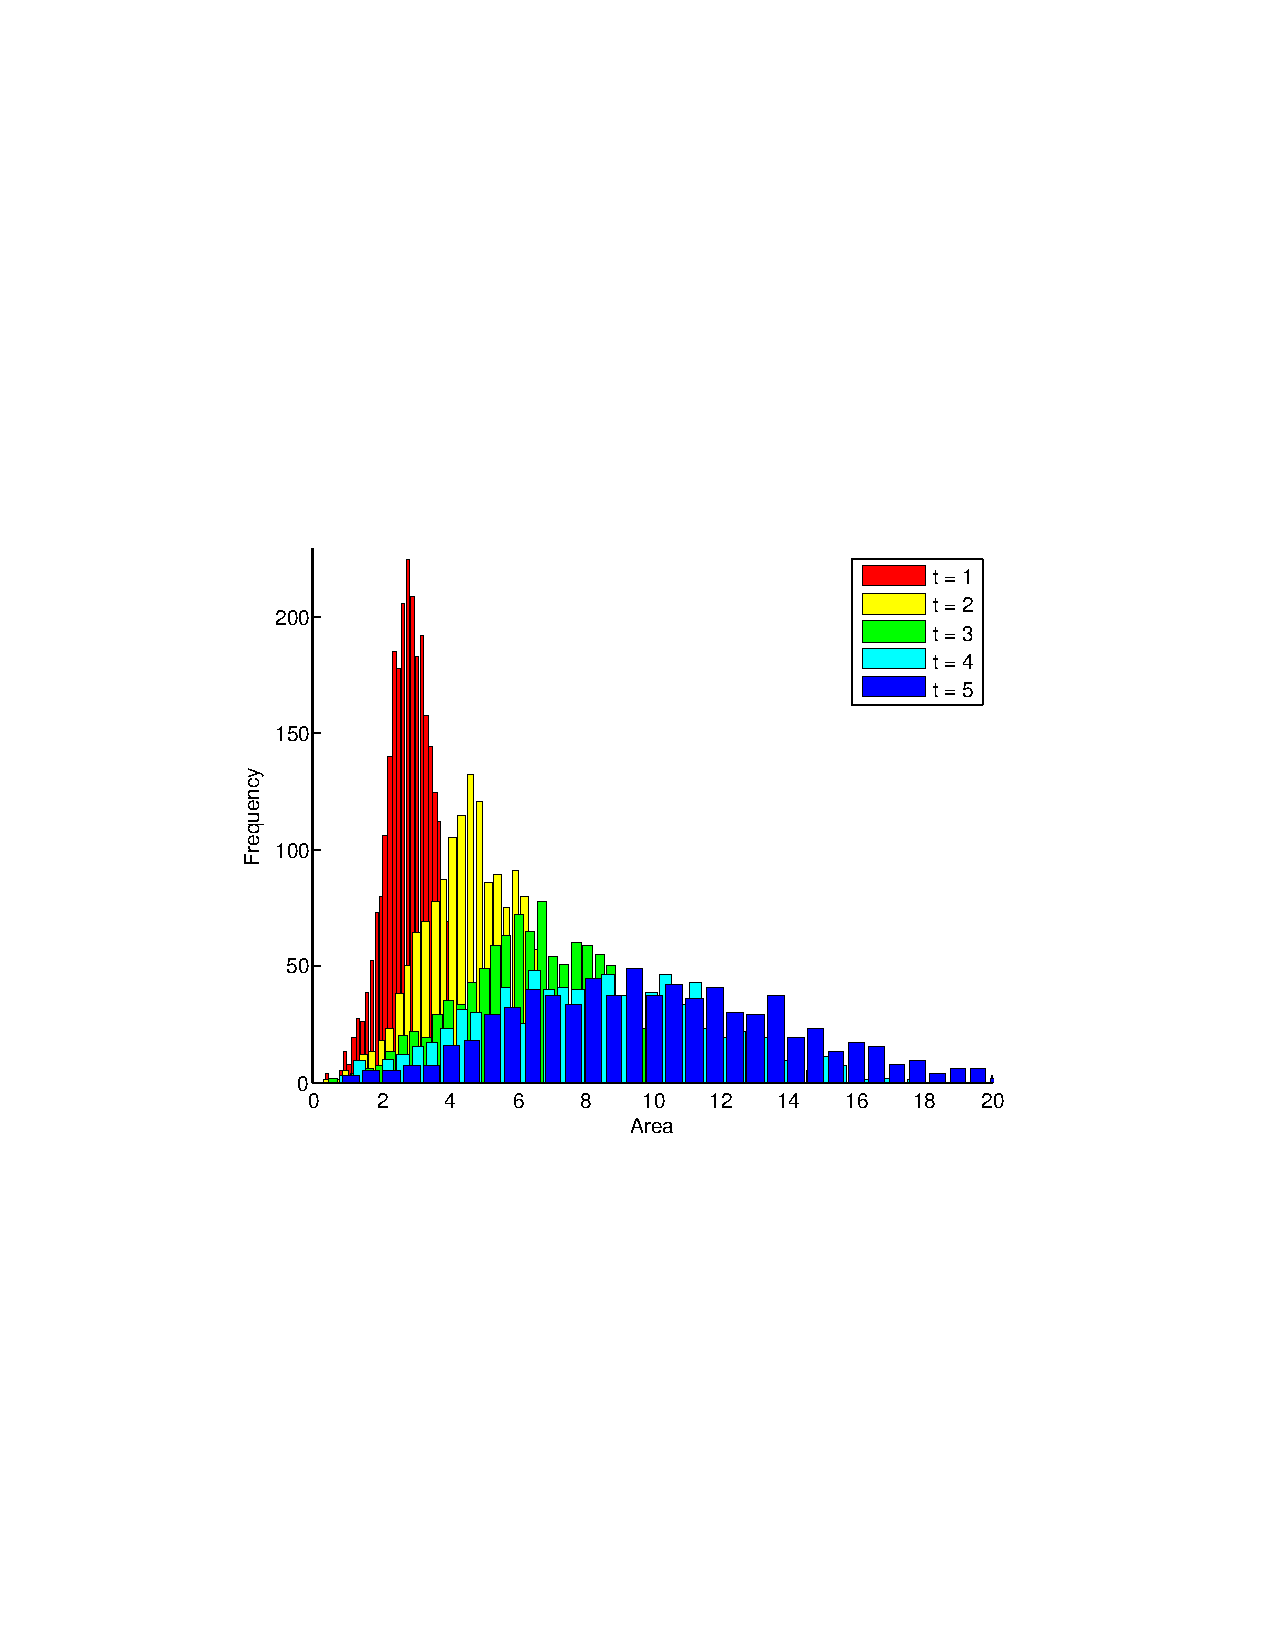
\includegraphics[width=\textwidth]{histbetatenthtier8.pdf}
\vspace{-130pt}
\caption{Histograms of eight-sided grain densities at $\beta = .1$.}
\end{figure}

\begin{figure}
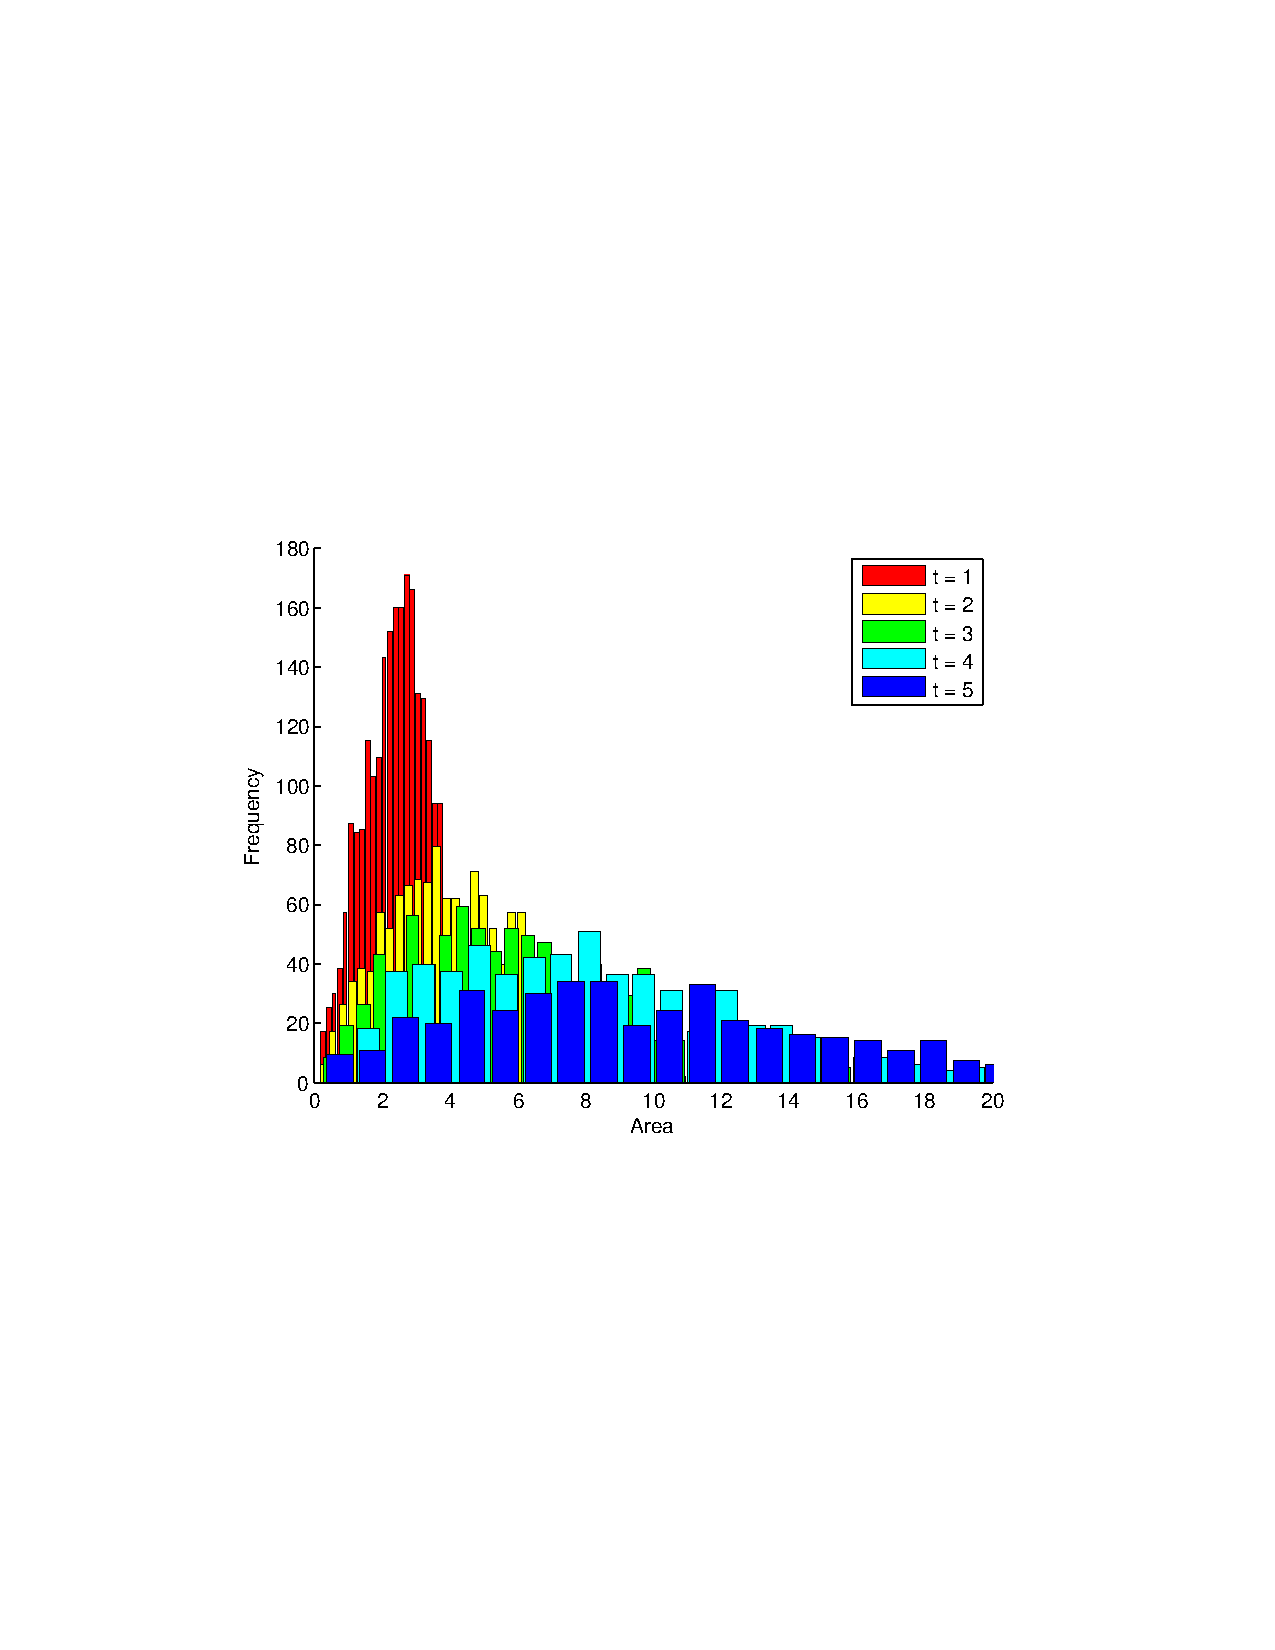
\includegraphics[width=\textwidth]{histbetaonetier8.pdf}
\vspace{-130pt}
\caption{Histograms of eight-sided grain densities at $\beta = 1$.}\label{tierdens9}
\end{figure}

\begin{figure}
\begin{centering}
\includegraphics[width=.5\textwidth]{averageareas.jpg}
\caption{Average areas of grains with sides 2-10 at $\beta= 0$.  Note how for each collection of $n$-gons,for $n= 2, \dots, M$, average area increases linearly.  Similar behavior holds for $\beta= .1$ and $\beta= 1.$}\label{averagewhole}
\end{centering}
\end{figure}

        
\begin{figure}
\centering
        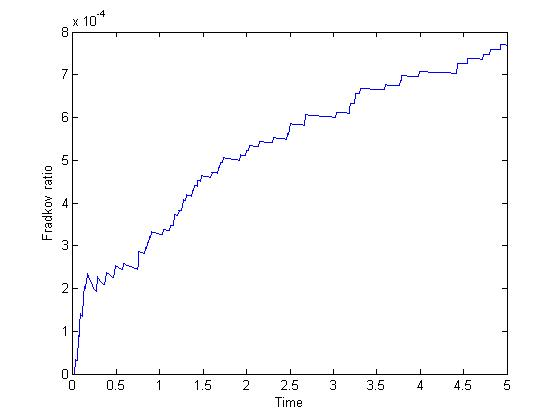
\includegraphics[width=.5\textwidth]{coarseratiobetazero.jpg}
        \caption{Side to grain deletion ratio $\gamma_\beta(t)$ at $\beta=.01$.}\label{fradrat1}
 \end{figure}
       
 \begin{figure}
        \centering
        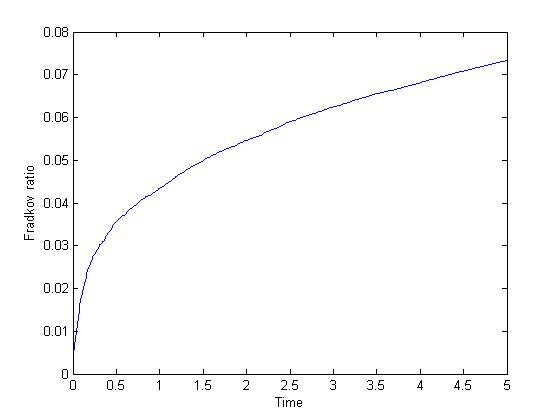
\includegraphics[width=.5\textwidth]{coarseratiobetatenth.jpg}
        \caption{Side to grain deletion ratio $\gamma_\beta(t)$ at $\beta=.1$.}
 \end{figure}       
        
        \begin{figure}
        \centering
        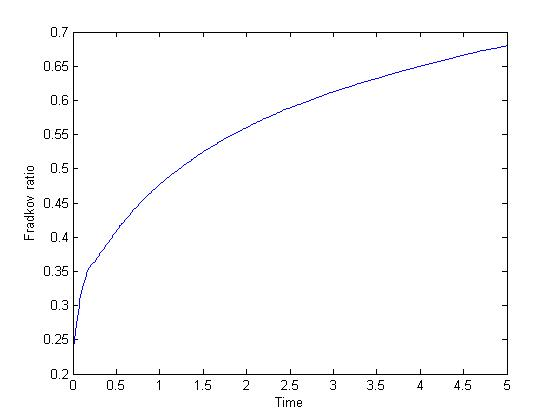
\includegraphics[width=.5\textwidth]{coarseratiobetaone.jpg}
        \caption{Side to grain deletion ratio $\gamma_\beta(t)$ at $\beta=1$.}\label{fradrat3}
       \end{figure}

\clearpage{}

 





\clearpage{\pagestyle{empty}\cleardoublepage}



\chapter{Conclusion}
\chapter{Conclusion}


\section{Future extensions}

\subsection{Garfield}

\begin{figure}
\centering

\includegraphics[width=1in]{garfield.pdf}
\caption{Garfield}
\end{figure}


\subsection{The Far Side}


\section{Alternative Perspectives}

Different, less mathematical perspectives on Peanuts have been
written. \cite{peanutsgospel}


\clearpage{\pagestyle{empty}\cleardoublepage}

% %------------------------ APPENDIX ------------------------%
% \appendix
% \chapter{A Comment on the $n-6$ Rule }
% %\lipsum[51-70]

% \clearpage{\pagestyle{empty}\cleardoublepage}


% \chapter{Uniqueness of  Solutions}
% \input{app3}
% \clearpage{\pagestyle{empty}\cleardoublepage}

%---------------------- BIBLIOGRAPHY ----------------------%

\bibliographystyle{siam}
\begin{spacing}{0.9}
  \bibliography{reference2}
\end{spacing}

\end{document}
